% =====================================================================
% Texto de qualificação — Mestrado Profissional em Ciências Ambientais
% PPGCIAMB / UFG — "A marcha ao norte" (LULC em Goiás, 1985–2024)
%
% Classe: abnTeX2 (ABNT NBR 14724) + abntex2cite alfabético (NBR 6023/10520)
% Compilação: .\compilar.ps1  (pdflatex -> bibtex -> pdflatex x2)
% =====================================================================
\documentclass[
  12pt,
  oneside,          % frente única (mudar p/ twoside na versão de depósito)
  a4paper,
  chapter=TITLE,
  section=TITLE,
  english,          % p/ o abstract
  brazil            % idioma principal (último = ativo)
]{abntex2}

% ---------------------------------------------------------------------
% Pacotes
% ---------------------------------------------------------------------
\usepackage[T1]{fontenc}
\usepackage[utf8]{inputenc}
\usepackage{newtxtext,newtxmath}  % Times (padrão visual acadêmico BR)
\renewcommand*\ttdefault{lmtt}    % typewriter da Latin Modern: tem itálico
                                  % real (a txtt inclinada vira bitmap e falha)
\usepackage{microtype}
\usepackage{indentfirst}   % recua também o 1o parágrafo após título. O default
                           % do LaTeX/memoir é não recuar (\noindentafterchapter);
                           % a prática brasileira recua todos, sem exceção.
\usepackage{graphicx}
\usepackage{booktabs}
\usepackage{xcolor}
\usepackage{placeins}      % \FloatBarrier. Usado SÓ no apêndice (o gerador o
                           % emite ao fim de cada seção): lá as tabelas são
                           % muitas e grandes, e sem barreira elas escorriam
                           % para dentro da seção seguinte — a Tabela da A.6
                           % saía depois de a A.7 já ter começado. Sem a opção
                           % [section], que valeria para o documento inteiro e
                           % mexeria na diagramação já conferida dos capítulos.
\usepackage[alf]{abntex2cite}   % citações ABNT autor-data

% Página de flutuante alinhada ao ALTO. Quando uma página contém só tabelas
% ("float page"), o default do LaTeX é \@fptop = 0pt plus 1fil, que distribui
% o vazio e empurra a tabela para o meio — no apêndice isso abria uma faixa
% branca de um terço de página acima de cada tabela grande. Com \@fptop = 0pt
% a tabela encosta no alto e o vazio sobra embaixo, onde não se lê como erro.
\makeatletter
\setlength{\@fptop}{0pt}
\setlength{\@fpsep}{14pt plus 1fil}
\setlength{\@fpbot}{0pt plus 1fil}
\makeatother

\graphicspath{{fig/}}

% Títulos em fonte 12 (padrão das normas universitárias BR: tamanho único,
% hierarquia por negrito/caixa alta; o default \Large do abnTeX2 destoa)
\renewcommand{\ABNTEXchapterfontsize}{\normalsize}
\renewcommand{\ABNTEXsectionfontsize}{\normalsize}
\renewcommand{\ABNTEXsubsectionfontsize}{\normalsize}
\renewcommand{\ABNTEXsubsubsectionfontsize}{\normalsize}
\renewcommand{\ABNTEXsubsubsubsectionfontsize}{\normalsize}

% Títulos em Times negrito, não em sans-serif. O abnTeX2 define
% \ABNTEXchapterfont = \sffamily; como newtxtext só troca a romana (corpo +
% math) e não a sans, os títulos vinham em Latin Modern Sans (Computer Modern)
% enquanto o corpo ficava em Times --- duas famílias visíveis. ABNT não exige
% sans nos títulos; negrito Times dá fonte única e é o padrão visual acadêmico.
% Seção/subseção/... herdam deste comando, assim como a capa, a folha de rosto
% e o título "Sumário".
\renewcommand{\ABNTEXchapterfont}{\normalfont\bfseries}

% Nota de trabalho: orientação visível no PDF sobre o que cada trecho
% ainda vai receber. Some quando o texto definitivo entrar no lugar.
% (nome \notaguia porque \nota já pertence ao abntex2cite)
\definecolor{notacinza}{gray}{0.40}
\newcommand{\notaguia}[1]{%
  \begin{quotation}\sloppy\small\itshape\color{notacinza}#1\end{quotation}}

% Linha de fonte sob a figura (ABNT NBR 14724: título acima, fonte abaixo,
% ambos em corpo menor). O minipage restaura o alinhamento à esquerda, que o
% \centering do ambiente figure desfaria.
\newcommand{\fontefig}[1]{%
  \par\vspace{-0.4\baselineskip}%
  \begin{minipage}{\textwidth}%
    \footnotesize\SingleSpacing\raggedright Fonte: #1%
  \end{minipage}}

% Nota da ilustração. A norma separa os dois campos: FONTE diz a procedência do
% dado; NOTA esclarece como ler a figura (convenção de classe, recorte, escala,
% o que uma linha pontilhada significa). Estavam os dois dentro de \fontefig, o
% que fazia a "fonte" ocupar meia dúzia de linhas de explicação metodológica.
\newcommand{\notafig}[1]{%
  \par\vspace{-0.2\baselineskip}%
  \begin{minipage}{\textwidth}%
    \footnotesize\SingleSpacing\raggedright Nota: #1%
  \end{minipage}}

% Caixa de destaque. Usada uma única vez, na abertura, para o endereço da
% visualização interativa. fbox+minipage em vez de um pacote de molduras:
% mantém a lista de pacotes enxuta e o traçado igual ao do resto do texto.
\newcommand{\destaque}[1]{%
  \begin{center}%
  \setlength{\fboxsep}{12pt}%
  \fbox{\begin{minipage}{0.90\textwidth}%
    \SingleSpacing\setlength{\parindent}{0pt}\small #1%
  \end{minipage}}%
  \end{center}}

% Ficha do levantamento (§2.10): obra localizada e ainda não lida. Traz forma
% bibliográfica completa para poder ser encontrada, e fica deliberadamente
% fora das referências --- nenhuma delas foi lida nem sustenta afirmação do
% texto. O verificar.py lê estas fichas para manter o §2.10 em sincronia com o
% bloco de lista de leitura do .bib; por isso uma ficha por comando.
\newcommand{\ficha}[1]{%
  \par\begingroup\small\SingleSpacing
  \hangindent=1.2em\hangafter=1\noindent #1\par\endgroup
  \vspace{2pt}}

% Endereço da visualização interativa, definido num só lugar.
\newcommand{\urlviz}{https://victorgit10.github.io/mestrado-lulc-goias/Visualizacao/}

% ---------------------------------------------------------------------
% Quadro como flutuante próprio. Convenção ABNT/IBGE adotada aqui: TABELA
% traz dado numérico tratado; QUADRO traz informação textual ou esquemática.
% A distinção é aplicada na designação, na numeração e na lista própria; a
% moldura fechada que a norma tabular do IBGE prevê para quadros NÃO foi
% adotada, para manter o mesmo traçado booktabs em todo o documento.
% O memoir fornece \newfloat e \newlistof; a extensão .loq guarda a lista.
% ---------------------------------------------------------------------
\newfloat[chapter]{quadro}{loq}{Quadro}
\newlistof{listofquadros}{loq}{Lista de Quadros}
\newlistentry[chapter]{quadro}{loq}{0}
\renewcommand{\cftquadroname}{Quadro\space}
\renewcommand*{\cftquadroaftersnum}{\hfill\textendash\hfill}  % igual ao abntex2
\counterwithout{quadro}{chapter}   % numeração corrida, como tabelas e figuras

% ---------------------------------------------------------------------
% Dados do trabalho
% ---------------------------------------------------------------------
\titulo{A marcha ao norte: dinâmica de uso e cobertura da terra em Goiás (1985--2024) e seus fatores socioeconômicos}
\autor{Victor Alves Rodrigues Amaral}
\local{Goiânia}
\data{2026}
\orientador{Prof. Dr. Laerte Guimarães Ferreira Júnior}
\instituicao{%
  Universidade Federal de Goiás\par
  Programa de Pós-Graduação em Ciências Ambientais --- PPGCIAMB}
\tipotrabalho{Texto de qualificação (Mestrado Profissional)}
\preambulo{Texto de qualificação apresentado ao Programa de Pós-Graduação em
Ciências Ambientais da Universidade Federal de Goiás, como requisito parcial
para a obtenção do título de Mestre em Ciências Ambientais.}

% Metadados do PDF
\makeatletter
\hypersetup{
  pdftitle={\@title},
  pdfauthor={\@author},
  pdfsubject={Uso e cobertura da terra em Goiás, 1985-2024},
  pdfkeywords={LULC, Cerrado, fronteira agrícola, Goiás, MapBiomas},
  colorlinks=true,
  linkcolor=blue!50!black,
  citecolor=blue!50!black,
  urlcolor=blue!50!black
}
\makeatother

% Espaçamento 1,5 no texto (padrão ABNT)
\OnehalfSpacing

% Recuo de parágrafo de 1,25 cm (convenção dos manuais universitários BR; o
% default herdado da memoir é ~0,62 cm, metade disso)
\setlength{\parindent}{1.25cm}

\begin{document}

\frenchspacing

% =====================================================================
% PRÉ-TEXTUAIS
% =====================================================================
\imprimircapa
\imprimirfolhaderosto

% !TEX root = ../main.tex
\setlength{\absparsep}{18pt}
\begin{resumo}
Este texto de qualificação examina a dinâmica de uso e cobertura da terra em
Goiás entre 1985 e 2024 e sua relação com fatores socioeconômicos, a partir da
série anual do MapBiomas (Coleção 10.1) para os 246 municípios goianos e de uma
malha de 166 Áreas Mínimas Comparáveis que garante território constante nas
análises longitudinais. Uma periodização orientada pelos dados divide os 40
anos em três atos (pastagem como herança, 1985--2000; expansão e
intensificação, 2001--2019; e conversão acelerada sob rótulo ambíguo,
2020--2024) e organiza o achado central: uma reorganização espacial da
conversão de terras em direção ao norte do estado (``a marcha ao norte''). A
investigação decompõe-se em quatro frentes: a existência do padrão
(deslocamento do centro de massa de cada uso da terra, que sobrevive a
verificações de pixel, malha, classe e barra de erro, com um gradiente
latitudinal que persiste nos quarenta anos); o mecanismo local, em que duas
lógicas convivem em todo o estado e a região explica pouco da idade da pastagem
convertida, ainda que a transição dominante seja de pastagem para lavoura no
Sul e de vegetação natural para pastagem no Norte; o teste formal do
deslocamento causal intraestadual, que não se confirma e tem como leitura
alternativa uma resposta coordenada a um \emph{driver} macroeconômico comum,
distribuída ao longo do gradiente Sul--Norte (evidência corroborante, não
estabelecida); e a desaceleração recente, compatível com o esgotamento da terra
ainda exposta à conversão no Sul, sustentada pela eliminação de hipóteses
concorrentes e por um mecanismo medido, a queda da taxa de conversão à medida
que a região se esgota. Apresentam-se a metodologia, os resultados
preliminares, os limites do que o trabalho afirma e o cronograma até a defesa.

\textbf{Palavras-chave}: uso e cobertura da terra; Cerrado; fronteira
agrícola; Goiás; MapBiomas.
\end{resumo}

\begin{resumo}[Abstract]
\begin{otherlanguage*}{english}
This qualifying text examines land use and land cover dynamics in the state of
Goiás, Brazil, between 1985 and 2024, and their relationship with socioeconomic
drivers, using the annual MapBiomas series (Collection 10.1) for the 246
municipalities of Goiás and a mesh of 166 Minimum Comparable Areas that keeps
territory constant in longitudinal analyses. A data-driven periodization
divides the 40 years into three acts --- pasture as inheritance (1985--2000),
expansion and intensification (2001--2019), and accelerated conversion
(2020--2024) --- and frames the central finding: a northward spatial
reorganization of land conversion within the state (``the northward march'').
The investigation unfolds along four fronts: the existence of the pattern
(displacement of the conversion center of mass, controlling for scale
effects); the local mechanism (two simultaneous logics --- intensification and
pasture-to-cropland substitution in the South, expansion over natural
vegetation in the North); a formal test of intra-state causal displacement,
which is not confirmed and points to an alternative reading as a coordinated
response to a common macroeconomic driver along the South--North gradient
(corroborating, not established, evidence); and the recent deceleration,
consistent with the exhaustion of land still exposed to conversion in the
South, supported both by the elimination of competing hypotheses and by a
measured mechanism, the decline in the conversion rate as a region is
depleted. The text presents the methodology,
preliminary results, the limits of what the work claims, and the schedule
until the defense.

\textbf{Keywords}: land use and land cover; Cerrado; agricultural frontier;
Goiás; MapBiomas.
\end{otherlanguage*}
\end{resumo}


\pdfbookmark[0]{\listfigurename}{lof}\listoffigures*\cleardoublepage
\pdfbookmark[0]{\listtablename}{lot}\listoftables*\cleardoublepage
\pdfbookmark[0]{Lista de Quadros}{loq}\listofquadros*\cleardoublepage

% !TEX root = ../main.tex
% LISTA DE ABREVIATURAS E SIGLAS
% Toda sigla aqui listada também é definida na primeira ocorrência no texto.
% Ordem alfabética (exigência da NBR 14724).
\begin{siglas}
  \item[ADF] Teste de raiz unitária de Dickey-Fuller aumentado
  \item[AMC] Área Mínima Comparável
  \item[APP] Área de Preservação Permanente
  \item[BACEN] Banco Central do Brasil
  \item[BIC] Critério de informação bayesiano
  \item[CO\textsubscript{2}e] Dióxido de carbono equivalente
  \item[EPSG] Código de sistema de coordenadas no registro geodésico \emph{EPSG Geodetic Parameter Dataset}
  \item[Embrapa] Empresa Brasileira de Pesquisa Agropecuária
  \item[HAC] Erro-padrão robusto a heterocedasticidade e autocorrelação
  \item[IBGE] Instituto Brasileiro de Geografia e Estatística
  \item[IC] Intervalo de confiança
  \item[IDH-M] Índice de Desenvolvimento Humano Municipal
  \item[IFDM] Índice FIRJAN de Desenvolvimento Municipal
  \item[iLUC] Mudança indireta de uso da terra (\emph{indirect land use change})
  \item[INPE] Instituto Nacional de Pesquisas Espaciais
  \item[IPCA] Índice Nacional de Preços ao Consumidor Amplo
  \item[IPEA] Instituto de Pesquisa Econômica Aplicada
  \item[KPSS] Teste de estacionariedade de Kwiatkowski-Phillips-Schmidt-Shin
  \item[LAPIG] Laboratório de Sensoriamento Remoto e Geoprocessamento (UFG)
  \item[LISA] Indicadores locais de associação espacial (\emph{local indicators of spatial association})
  \item[MATOPIBA] Fronteira agrícola formada por Maranhão, Tocantins, Piauí e Bahia
  \item[MAUP] Problema da unidade de área modificável (\emph{modifiable areal unit problem})
  \item[Mha] Milhão de hectares
  \item[Mt] Milhão de toneladas
  \item[PAM] Produção Agrícola Municipal (IBGE)
  \item[PIB] Produto Interno Bruto
  \item[PPGCIAMB] Programa de Pós-Graduação em Ciências Ambientais (UFG)
  \item[PPM] Pesquisa da Pecuária Municipal (IBGE)
  \item[PRODES] Sistema de monitoramento do desmatamento por satélite (INPE)
  \item[SAR] Modelo espacial autorregressivo, de defasagem espacial (\emph{spatial autoregressive})
  \item[SEM] Modelo de erro espacial (\emph{spatial error model})
  \item[SICOR] Sistema de Operações do Crédito Rural e do Proagro (BACEN)
  \item[SIDRA] Sistema IBGE de Recuperação Automática
  \item[SIRGAS] Sistema de Referência Geocêntrico para as Américas
  \item[STARS] Detector sequencial de mudança de regime, de Rodionov
  \item[UFG] Universidade Federal de Goiás
  \item[USDA-ERS] Serviço de Pesquisa Econômica do Departamento de Agricultura dos Estados Unidos
  \item[VIF] Fator de inflação de variância
\end{siglas}


\pdfbookmark[0]{\contentsname}{toc}
\tableofcontents*
\cleardoublepage

% =====================================================================
% TEXTUAIS
% =====================================================================
\textual

\chapter*{Apresentação --- memorial}
\phantomsection\addcontentsline{toc}{chapter}{APRESENTAÇÃO --- MEMORIAL}
% \chapter* não atualiza a marca de cabeçalho (só a versão numerada o faz), e
% sem isto as páginas seguintes herdam o "SUMÁRIO" da seção anterior.
\markboth{Apresentação --- memorial}{Apresentação --- memorial}

\section*{Trajetória e formação}

Sou graduado em Ciências Econômicas pela Universidade Federal de Goiás
(UFG, 2024). Ainda durante a graduação, em 2023, ingressei no Laboratório de
Sensoriamento Remoto e Geoprocessamento (LAPIG/UFG) como bolsista, para atuar
no apoio à gestão de projetos. Aos poucos, além das atividades de gestão,
passei a integrar também atividades de pesquisa, fazendo parte da equipe do
projeto Pasto Legal (\textit{pasto.legal}) e realizando trabalhos de
desenvolvimento de automações, sites e ferramentas para o laboratório.

A convivência diária com um laboratório de referência em sensoriamento remoto
moldou minha formação complementar. Em 2025, realizei o Geocurso de
Classificação de Imagens com Google Earth Engine, ministrado no LAPIG pelo
pesquisador Bernard Oliveira. Em 2026, realizei o Geocurso Explorando
Embeddings Geoespaciais com Modelos Fundacionais (Clay e AlphaEarth),
ministrado pelo pesquisador Tiago Gonçalves Maia Geraldine. Ainda em 2026,
ministrei no LAPIG um curso de extensão sobre automação de fluxos de trabalho
com Google Apps Script, GitHub Actions e inteligência artificial, transferindo
para outros a prática que eu vinha construindo.

\section*{O percurso do mestrado}

Cheguei ao Programa de Pós-Graduação em Ciências Ambientais (PPGCIAMB) pela
relação estreita entre o LAPIG e o programa. O tema --- a dinâmica das
pastagens em Goiás e seus fatores socioeconômicos --- está no encontro
natural entre a minha formação de economista e a tradição do laboratório no
monitoramento do uso da terra, especialmente no mapeamento de pastagens.

A pesquisa começou com uma hipótese clássica: a pastagem como estágio
intermediário da ocupação (vegetação $\to$ pasto $\to$ lavoura). O que ela
se tornou foi decidido pelos dados. O percurso está documentado em 54
pipelines de análise, com índice lógico, narrativa de construção e um
registro de decisões metodológicas numeradas --- e foi esse percurso
exploratório, com suas confirmações e refutações, que fez emergir a tese da
``marcha ao norte'' apresentada neste texto. Esta dissertação nasce, assim,
da vontade de contar as histórias que a série riquíssima de quatro décadas do
MapBiomas guarda. Nesse caminho, os dados do Instituto Brasileiro de
Geografia e Estatística (IBGE) também foram fundamentais, tanto para
construir a narrativa central quanto para revelar faces que os mapas sozinhos
não mostram.

\section*{O método de trabalho e o uso de inteligência artificial}

Devo registrar com franqueza o meu ponto de partida: cheguei ao mestrado sem
experiência prática de programação --- apenas noções básicas de lógica, R e
Python --- e sem bagagem em geotecnologias. A ponte foi construída pela
inteligência artificial. A partir de 2026, com o apoio e o incentivo do
LAPIG, em especial do professor Laerte, comecei a integrar ferramentas de IA
aos fluxos da gestão financeira dos projetos do laboratório; à medida que
ganhei fluência, levei essa prática para o centro da pesquisa.

O fluxo de trabalho que desenvolvi pode ser descrito assim: a curiosidade
vem primeiro; dela nasce uma pergunta formulada com precisão; a IA me ajuda
a materializar os scripts necessários para buscar a resposta nos dados; e,
encontrado um achado, a IA me ajuda a materializar visualizações ---
inclusive interativas --- que o tornem legível e verificável. As perguntas,
as decisões metodológicas e a interpretação dos resultados permanecem
minhas; o que a IA me fornece é autonomia para programar no ritmo da
curiosidade.

Essa autonomia cobra uma contrapartida de rigor, e a pesquisa a paga de
forma auditável: um diário de 27 decisões metodológicas numeradas
(Apêndice~\ref{ap:decisoes}), auditorias sistemáticas que rastreiam cada
número exibido até o arquivo de dados que o gerou, e autocorreções
documentadas --- resultados que seriam publicados e foram superados por um
teste a mais. A transparência operacional desse arranjo está declarada na
metodologia (seção~\ref{sec:met-ia}); o que pertence a este memorial é o seu
sentido formativo: foi por esse caminho que a curiosidade de um economista
ganhou os instrumentos para interrogar quarenta anos de mapas.
   % Memorial (não numerado)
\chapter{Introdução}
\label{cap:introducao}

\notaguia{Primeira redação, a partir da ``tese em uma página'' do guia de
leitura, da abertura da visualização e do escopo original. Números aqui são
de enquadramento (período, unidades, atos); os resultados quantitativos
moram no Capítulo~\ref{cap:resultados}.}

\section{Contexto e problema}
\label{sec:intro-contexto}

O Cerrado é a fronteira ativa da agricultura brasileira, e Goiás está no
coração do bioma. A série anual do MapBiomas (Coleção 10.1) permite observar,
ano a ano e pixel a pixel, o que cada fração do território goiano foi entre
1985 e 2024 --- pastagem, lavoura, vegetação natural, área urbana --- e,
portanto, reconstituir quatro décadas de transformação da paisagem com uma
resolução que era impensável há pouco tempo.

O que essa série mostra para Goiás não é uma história simples de avanço de
fronteira. O estado já entra na série amplamente ocupado: a pastagem que
domina a paisagem de 1985 é herança das frentes de ocupação anteriores. O
que as quatro décadas seguintes registram é uma \emph{reorganização}
profunda e espacialmente estruturada desse território já ocupado: no Sul, a
pastagem cede lugar à lavoura e a produção se intensifica; no Norte, a
fronteira segue ativa, convertendo vegetação natural em pasto. O resultado
agregado é que lavoura, pastagem e rebanho deslocam-se gradualmente para o
norte do estado --- o fenômeno que este trabalho chama de ``marcha ao
norte''.

O problema de pesquisa é duplo: descrever esse padrão com precisão --- ele
existe, é robusto, em que ritmo avança? --- e explicar o que o coordena.
Três famílias de explicação concorrem: uma região empurrando a outra (o
deslocamento indireto de uso da terra); forças de mercado comuns atuando
sobre um gradiente natural de aptidão; e o próprio encolhimento do que resta
exposto à conversão. Distinguir entre elas exige mais que
mapas: exige o cruzamento sistemático da série de uso da terra com as
variáveis socioeconômicas --- produto agropecuário, crédito rural, rebanho,
preços de commodities, câmbio --- e um desenho analítico capaz de rejeitar
as explicações que não se sustentam.

\section{Pergunta e objeto}
\label{sec:intro-pergunta}

A pergunta central é: \emph{como e por que o uso da terra mudou em Goiás
entre 1985 e 2024?} --- e, em sua forma mais aguda: \emph{o que coordena a
reorganização espacial da produção agropecuária no estado?}

O objeto empírico são os 246 municípios goianos, observados anualmente ao
longo de 40 anos. Para as análises longitudinais, os municípios são
agregados em 166 Áreas Mínimas Comparáveis, malha que mantém o território
constante diante das emancipações municipais do período
(Capítulo~\ref{cap:metodologia}). Sobre essa base, a série de uso e
cobertura da terra é cruzada com o painel socioeconômico municipal.

A investigação partiu de uma hipótese clássica --- a pastagem como estágio
intermediário da ocupação (vegetação $\to$ pasto $\to$ lavoura), com a
lavoura do Sul empurrando a pecuária para o Norte do próprio estado --- e a
trajetória da pesquisa foi, em boa medida, o teste dessa hipótese. Parte
dela se confirmou; a parte mais tentadora, não. O deslocamento causal de uma
região sobre a outra, testado formalmente, não se sustentou, e o que emergiu
em seu lugar foi a leitura que estrutura este texto: duas dinâmicas
paralelas --- intensificação no Sul, fronteira no Norte --- movidas pelo
mesmo motor econômico sobre um gradiente de aptidão, e limitadas por um teto
de oferta de terra convertível. Vários dos resultados centrais do trabalho
são, assim, resultados nulos documentados: afirmações sobre o que os dados
mostram que \emph{não} acontece.

\section{Justificativa}
\label{sec:intro-justificativa}

A lacuna científica é de escala e de desenho. A literatura empírica da
fronteira do Cerrado opera majoritariamente na escala do bioma e das suas
grandes regiões --- com o MATOPIBA, acrônimo que designa a fronteira agrícola
formada por Maranhão, Tocantins, Piauí e Bahia, como caso paradigmático --- e a
literatura de mudança indireta de uso da terra (iLUC, do inglês \emph{indirect
land use change}) estabelece o fenômeno entre regiões e
biomas \cite{Lapola2010, Arima2011}. O canal \emph{intra-estadual} --- uma
região de um mesmo estado empurrando a fronteira da outra --- raramente é
isolado e testado, e as séries municipais longas costumam ignorar o problema
das fronteiras administrativas móveis. Este trabalho contribui exatamente
nesse ponto: alta resolução espacial, território constante e um teste formal
do canal de deslocamento local (Capítulo~\ref{cap:referencial}).

A relevância ambiental é direta: o Cerrado remanescente de Goiás
concentra-se no Norte do estado --- precisamente a região para onde a
conversão migrou. Compreender o que move essa conversão, e em que ritmo,
é condição para dimensionar a exposição da vegetação que resta. Para
políticas públicas, a distinção importa na prática: se a conversão no Norte
fosse efeito-dominó da lavoura do Sul, conter a lavoura conteria a
fronteira; se, como os resultados sugerem sem ainda estabelecer, ambas
respondem a um drive de mercado comum, as alavancas eficazes são outras ---
e agem sobre o estado inteiro.

Por fim, no espírito do mestrado profissional, o trabalho gera produtos de
uso direto: um conjunto reproduzível de pipelines de coleta e análise sobre
dados públicos e uma visualização interativa que torna os achados
navegáveis por não especialistas.

\section{Objetivos}
\label{sec:intro-objetivos}

O objetivo geral é caracterizar e explicar a reorganização espacial do uso e
cobertura da terra em Goiás entre 1985 e 2024, em sua relação com fatores
socioeconômicos.

Os objetivos específicos espelham as quatro frentes da investigação:

\begin{enumerate}
  \item caracterizar o padrão espaço-temporal da conversão de terras e
        verificar a existência, o ritmo e a robustez do deslocamento da
        fronteira para o norte;
  \item identificar os mecanismos locais que sustentam o padrão ---
        intensificação e substituição pasto$\to$lavoura no Sul,
        extensificação sobre vegetação natural no Norte;
  \item testar formalmente a hipótese de deslocamento intra-estadual e
        avaliar o papel de drivers macroeconômicos comuns, com destaque
        para o câmbio;
  \item examinar a desaceleração recente da conversão e a hipótese do teto
        de oferta de terra convertível no Sul do estado.
\end{enumerate}

\section{Organização do documento}
\label{sec:intro-organizacao}

O texto está organizado em seis capítulos, precedidos por um memorial. O
Capítulo~\ref{cap:referencial} situa a investigação na literatura da
fronteira agrícola, do deslocamento indireto de uso da terra, da
intensificação e dos drivers macroeconômicos. O
Capítulo~\ref{cap:metodologia} apresenta as fontes de dados, as unidades de
análise, a construção do painel e as decisões metodológicas críticas ---
inclusive o papel da inteligência artificial como instrumento de pesquisa.
O Capítulo~\ref{cap:resultados} apresenta os resultados preliminares em duas
camadas: a periodização dos 40 anos em três atos (1985--2000, 2001--2019,
2020--2024) e as quatro frentes de evidência da marcha ao norte. O
Capítulo~\ref{cap:discussao} posiciona os achados na literatura e consolida
alcance e limites, e o Capítulo~\ref{cap:cronograma} apresenta o cronograma
até a defesa.

\chapter{Referencial teórico}
\label{cap:referencial}

\section{O estatuto deste capítulo}
\label{sec:ref-estatuto}

A investigação não partiu de um arcabouço teórico em busca de confirmação
empírica. Partiu de uma pergunta sobre a dinâmica da pastagem em Goiás e
avançou pela curiosidade: cada resposta abria a pergunta seguinte, e foi essa
cadeia --- não uma hipótese teórica prévia --- que produziu as quatro frentes
da investigação e a tese da ``marcha ao norte''. A literatura foi mobilizada,
nesse percurso, sobretudo para decidir \emph{como perguntar}: qual estimador
resiste a séries integradas, qual teste de quebra não depende de datas
escolhidas pelo pesquisador, que unidade territorial permite comparar
municípios ao longo de quatro décadas. É desse uso que vem o instrumental do
Capítulo~\ref{cap:metodologia}.

O estágio atual é outro. Existem respostas, e falta a leitura sistemática que
diga o que a literatura já sabe sobre elas. Essa leitura é trabalho da
dissertação. A Seção~\ref{sec:ref-confrontados} reúne os arcabouços que os
dados já confrontaram --- cada um com uma previsão específica que a
investigação pôde testar, inclusive quando o teste a contrariou --- e a
Seção~\ref{sec:ref-agenda}, os que permanecem como agenda de leitura.

\section{A tese e os arcabouços que ela mobiliza}
\label{sec:ref-tese}

A tese que este trabalho defende pode ser enunciada em uma frase: Goiás
viveu, entre 1985 e 2024, uma reorganização espacial da produção
agropecuária --- intensificação no Sul, fronteira no Norte --- compatível com
a ação de forças de mercado comuns sobre um gradiente de aptidão, e limitada
pelo encolhimento da terra ainda exposta à conversão; e \emph{não} um
deslocamento causal de uma região sobre a outra. Das três cláusulas, a
segunda é a que o trabalho estabelece com mais firmeza --- é a que se testa
diretamente e cujo resultado é negativo ---, enquanto a leitura de mercado
comum permanece corroborante e não estabelecida.

Cada termo dessa frase pede um arcabouço próprio: \emph{fronteira} e
\emph{reorganização} remetem à teoria da fronteira agrícola; \emph{gradiente
de aptidão}, à economia da renda da terra; \emph{deslocamento causal}, à
literatura de mudança indireta de uso da terra (iLUC) e de teleacoplamento;
\emph{forças de mercado}, aos drivers macroeconômicos das commodities; e
\emph{teto de oferta}, à teoria da transição florestal. Nem todos foram
percorridos com a mesma profundidade, e a seção seguinte trata apenas
daqueles em que houve confronto efetivo com o dado.

\section{Os arcabouços e as previsões que eles geram}
\label{sec:ref-confrontados}

O critério de inclusão nesta seção é estreito e deliberado: entra o arcabouço
do qual foi possível extrair uma previsão específica, verificável na série de
Goiás. O que se enuncia aqui é a previsão; o resultado de cada confronto ---
que em dois dos cinco casos não foi favorável ao arcabouço --- está no
Capítulo~\ref{cap:discussao}, e cada subseção indica onde.

\subsection{Renda da terra e localização}
\label{sec:ref-renda}

A base espacial do argumento é o modelo de localização agrícola de von Thünen
(1826), para o qual a terra é alocada ao uso que lhe rende mais, e a renda de
cada uso é determinada pela localização. Dessa formulação decorre uma
previsão testável: a expansão agrícola ocupa primeiro as terras de melhor
aptidão e só depois as piores --- e, portanto, os usos devem ordenar-se no
espaço segundo o gradiente de aptidão.

Testar isso exige medir o gradiente por fora do fenômeno que ele deveria
explicar. Inferir aptidão a partir do uso observado seria circular; a
alternativa adotada, um mapa edafoclimático construído sobre atributos
físicos, é descrita no Capítulo~\ref{cap:metodologia}.

\citeonline{Angelsen2007} oferece a síntese que amarra a dimensão espacial à
temporal, ao combinar explicitamente von Thünen com a transição florestal: a
renda agrícola crescente eleva o desmatamento até que o próprio
desenvolvimento a reduza, ou até que a escassez de vegetação eleve a renda do
remanescente e reverta a trajetória. A previsão que daí se extrai é a de que
o gradiente espacial e o pico temporal sejam faces do mesmo processo de renda
da terra, e não dois fenômenos distintos. O confronto está na
Seção~\ref{sec:disc-fronteira}.

\subsection{Transição florestal}
\label{sec:ref-transicao}

A teoria da transição florestal \cite{Mather1992, Rudel2005} descreve uma
trajetória em três fases: cobertura alta e desmatamento baixo, conversão
acelerada, e por fim estabilização ou ganho líquido de vegetação. É o
arcabouço com que a pesquisa lê o ``teto de oferta'': o Sul do estado, que
abriu cedo, deveria comportar-se como região em fase tardia, enquanto no
Norte resta Cerrado ainda exposto à conversão.

A previsão que interessa é a da fase tardia, e ela tem duas metades: estoque
reduzido com taxa de conversão cadente, \emph{e} uma virada de sinal ---
recuperação, regeneração líquida da vegetação. As duas metades são
separáveis no dado, e essa separação é o que a Seção~\ref{sec:disc-fronteira}
examina. Se a resposta for peculiaridade do Cerrado, do período ou do estado,
este desenho não decide --- pergunta que a agenda da
Seção~\ref{sec:ref-agenda} precisa endereçar.

\subsection{Deslocamento indireto e teleacoplamento}
\label{sec:ref-iluc}

A literatura de mudança indireta de uso da terra estabelece que a expansão da
soja desloca a pecuária e, com ela, a fronteira. \citeonline{Lapola2010}
mostram que esse efeito indireto pode anular a economia de carbono dos
biocombustíveis brasileiros, ao empurrar a fronteira de pastagem para as
florestas amazônicas e para o Cerrado; \citeonline{Arima2011} oferecem
confirmação estatística do mecanismo na Amazônia, estimando que uma redução
de 10\% da soja em áreas de pasto consolidado teria reduzido o desmatamento
em até 40\% nos municípios mais florestados. O fenômeno é real na escala em
que foi estabelecido --- entre regiões e entre biomas.

A previsão que este trabalho pôde testar é mais estreita, e essa literatura
não a isola: o deslocamento \emph{intra-estadual} --- a lavoura do Sul goiano
empurrando o pasto para o Norte do próprio estado, por adjacência e com
precedência temporal curta.

Havia razão teórica para esperá-lo, e convém registrá-la antes do resultado.
\citeonline{Meyfroidt2010} definem \emph{leakage} como ``o deslocamento do
desmatamento para localidades vizinhas, por migração dos agentes do
desmatamento ou por comércio'': a vizinhança está no enunciado, e a migração
de agentes opera a curta distância. O arcabouço do teleacoplamento
\cite{Liu2013}, por sua vez, define seu objeto como as interações \emph{a
distância} e põe os acoplamentos locais de lado --- não prevê, portanto, a
ausência de efeito de vizinhança. E o precedente mais próximo,
\citeonline{Arima2011}, opera justamente no nível do município brasileiro,
com matrizes de peso espacial, e encontrou o efeito. O confronto está na
Seção~\ref{sec:disc-iluc}.

\subsection{Intensificação e disputa por terra}
\label{sec:ref-intensificacao}

Para a pecuária brasileira, \citeonline{Cohn2014} examinam, com um modelo
econômico de uso global da terra, se políticas de intensificação poderiam
poupar floresta e reduzir emissões. Dois de seus resultados oferecem previsão
verificável aqui. O primeiro é que a terra poupada fica bem aquém do
proporcional ao ganho de produtividade: a poupança existe, mas é parcial. O
segundo é locacional --- sob as políticas simuladas, a pastagem intensiva tem
cerca do dobro da chance da pastagem convencional de se instalar justamente
nas terras de melhor aptidão e logística para soja, de modo que a
intensificação da pecuária tende a \emph{competir} com a expansão da lavoura
pela mesma terra. Essa disputa, projetada ali em cenário, pode aqui ser
observada como desfecho medido no dado municipal
(Seção~\ref{sec:disc-iluc}).

\subsection{O câmbio e a divisão de trabalho com a literatura}
\label{sec:ref-cambio}

\citeonline{Richards2012} constituem a referência-âncora do driver cambial: a
desvalorização das moedas locais no fim dos anos 1990 elevou o retorno
esperado da soja e disparou resposta de oferta em área. Os autores estimam
que da ordem de 80~mil~km$^2$ --- 31\% da extensão então cultivada em Brasil,
Bolívia e Paraguai --- surgiram como resposta às desvalorizações do período;
só no Brasil, 63~mil~km$^2$, ou 29\% da área nacional de 2009.

O que este trabalho pode acrescentar a isso é limitado por construção, e o
limite precisa ser dito aqui para que o Capítulo~\ref{cap:resultados} seja
lido na chave certa. Com efeito fixo de ano, o painel absorve o nível do
choque comum e só deixa estimável o \emph{gradiente}: se o mesmo choque
desloca a atividade para onde a aptidão é \emph{menor}, com o núcleo apto
respondendo em lavoura e a fronteira, em gado. A divisão de trabalho é,
portanto, explícita: é a literatura que carrega o nível causal
câmbio$\to$soja$\to$fronteira, já ancorado em escala nacional e continental;
a tese contribui com a geografia desse efeito dentro do estado, e não
poderia contribuir com mais. O peso do que se obteve está na
Seção~\ref{sec:disc-drive}.

\subsection{O espelho do Cerrado}
\label{sec:ref-matopiba}

A literatura empírica mais diretamente comparável é a da fronteira do
Cerrado. \citeonline{Soterroni2019}, ao avaliar a extensão da Moratória da
Soja ao bioma, consolidam o Cerrado como fronteira ativa da agricultura
brasileira, com a expansão concentrando-se no norte e nordeste --- a região
do MATOPIBA (Maranhão, Tocantins, Piauí e Bahia), que nas projeções dos
autores absorve 86\% da expansão da soja no bioma até 2050 e concentra a
maior parte da conversão de vegetação natural para soja, por ser onde restam
os maiores remanescentes não perturbados. Como magnitude observada do
fenômeno, \citeonline{Rausch2019} estimam que a conversão direta para soja
respondeu por 16 a 32\% do desmatamento anual do Cerrado entre 2003 e 2014.

O achado-espelho decisivo para o posicionamento é a composição dessa
expansão, e ele está em \citeonline{CarneiroFilho2016}: de 2000 a 2014 a área
agrícola do Cerrado cresceu 87\%, e essa expansão se deu essencialmente sobre
áreas já antropizadas --- em torno de 70\% do total no período, chegando a
74\% na década final, com mais da metade sobre pastagem.
A exceção é o MATOPIBA que, ``por não dispor de áreas antropizadas com
aptidão para a agricultura, teve a maioria da expansão sobre áreas de
vegetação nativa''. Como a soja responde por 90\% da área agrícola do bioma,
a dinâmica descrita é, na prática, a da soja.

A previsão, para um estado que atravessa o mesmo bioma no eixo Sul--Norte, é
a de que esse contraste entre Cerrado maduro e fronteira apareça dentro de
Goiás --- e, aqui, sob um único desenho analítico, na mesma malha e com o
mesmo classificador (Seção~\ref{sec:disc-matopiba}).

\section{A linhagem do centróide migratório}
\label{sec:ref-centroide}

A métrica-manchete da primeira frente --- o centro de massa da conversão e
seu deslocamento --- pertence a uma linhagem metodológica consolidada, e não
é construção ad hoc. A elipse de desvio-padrão foi formalizada por
\citeonline{Lefever1926} e atualizada como instrumento de descrição espacial
por \citeonline{Yuill1971}; o centro mediano, obtido pelo algoritmo de
Weiszfeld, completa o instrumental clássico da estatística espacial
descritiva. Essa linhagem responde à objeção de ``métrica caseira'' e situa a
escolha metodológica do Capítulo~\ref{cap:metodologia}.

\section{Agenda de leitura para a dissertação}
\label{sec:ref-agenda}

Cada item traz a fonte identificada e a pergunta que a leitura deve decidir.

\begin{description}\itemsep2pt
\item[Intensificação induzida pela demanda.] Boserup (1965); Strassburg \emph{et al.}
(2014). \textbf{Decide:} se o regime do Sul é intensificação induzida por demanda ou
substituição por renda da terra, e se os dois são distinguíveis com os dados disponíveis.
\item[Deslocamento em escala subnacional.] Levantamento a partir de
\citeonline{Arima2011}, precedente já conhecido; Seto \emph{et al.} (2012) na fila.
\textbf{Decide:} se o nulo obtido aqui diverge de um resultado consolidado, replica um
nulo já reportado, ou não encontra par.
\item[Transição florestal, revisitada.] Literatura posterior a \citeonline{Rudel2005},
sobre savanas tropicais. \textbf{Decide:} se a estabilização sem recuperação observada no
Sul é caso conhecido do arcabouço ou observação a registrar.
\item[Fronteira na tradição brasileira.] Martins (1971); Becker. \textbf{Decide:} se as
categorias sociológicas admitem correspondência com cobertura do solo, ou se o uso é
analógico --- como a Seção~\ref{sec:disc-fronteira} já supõe.
\item[Composição da expansão no Cerrado.] Spera \emph{et al.} (2016); Noojipady \emph{et
al.} (2017). \textbf{Decide:} se as estimativas de \citeonline{CarneiroFilho2016}
convergem com as de bases independentes.
\item[Centróides migratórios em uso da terra.] \textbf{Decide:} se a métrica tem
precedente em matrizes de transição, o que mudaria como defendê-la.
\item[Câmbio, período recente.] Estudos do USDA-ERS sobre a depreciação de 2015--2016.
\textbf{Decide:} se o mecanismo de \citeonline{Richards2012} se repete no episódio
recente.
\item[Fronteira agrícola em Goiás.] Produção da UFG e da literatura regional.
\textbf{Decide:} o que já está estabelecido para Goiás, e portanto o que aqui é
contribuição.
\item[Von Thünen no original.] \textbf{Decide:} se a leitura corrente do modelo é fiel à
formulação.
\end{description}

\section{Síntese e posicionamento provisório}
\label{sec:ref-sintese}

O Quadro~\ref{quadro:posicionamento} resume o posicionamento na literatura
efetivamente conferida. É provisório por construção: a agenda da
Seção~\ref{sec:ref-agenda} pode alterar tanto as âncoras quanto a avaliação
do que a pesquisa acrescenta.

\begin{quadro}[htb]
\centering
\caption[Posicionamento provisório na literatura, por frente]{Posicionamento provisório na literatura conferida, por frente da
investigação.}
\label{quadro:posicionamento}
\small
\begin{tabular}{p{2.4cm}p{3.2cm}p{2.9cm}p{5.4cm}}
\toprule
\textbf{Frente} & \textbf{Arcabouço} & \textbf{Âncoras conferidas} & \textbf{O que o confronto mostrou} \\
\midrule
1. O padrão (a marcha) & centro de gravidade; renda da terra &
\citeonline{Lefever1926}; \citeonline{Yuill1971}; \citeonline{Angelsen2007} &
quantifica a marcha e o gradiente latitudinal persistente, com controle do
efeito de escala; a premissa de aptidão é medida por fonte exógena \\
\addlinespace
2. Mecanismo local duplo & intensificação $\times$ extensificação &
\citeonline{Cohn2014} &
a disputa por terra projetada em cenário aparece resolvida no dado municipal,
a favor da lavoura \\
\addlinespace
3a. Deslocamento (nulo) & iLUC; teleacoplamento; \emph{leakage} &
\citeonline{Lapola2010}; \citeonline{Arima2011}; \citeonline{Liu2013};
\citeonline{Meyfroidt2010} &
testa o canal em Goiás sob adjacência dirigida e não o encontra; o arcabouço
não previa esse nulo, e o precedente subnacional mais próximo
(\citeonline{Arima2011}) encontrou o efeito em outra região, desfecho e
especificação \\
\addlinespace
3b. Drive comum & drivers macro de commodities &
\citeonline{Richards2012} &
a literatura carrega o nível causal; o painel só estima o gradiente, e como
corroborante, não estabelecido \\
\addlinespace
4. Teto de oferta & transição florestal &
\citeonline{Mather1992}; \citeonline{Rudel2005} &
a previsão de recuperação na fase tardia \emph{não} se cumpre: estabilização
por depleção, sem regeneração líquida \\
\bottomrule
\end{tabular}
\fontefig{elaboração própria, a partir das obras conferidas em \texttt{ref/pdf/}.}
\end{quadro}

À pergunta ``o que há de novo, se a fronteira do Cerrado rumo ao norte já é
conhecida?'', a resposta provisória é: a literatura conferida documenta a
marcha da fronteira do bioma e o deslocamento indireto entre regiões; esta
pesquisa leva essas leituras à alta resolução intra-estadual, sobre malha de
território constante, e testa formalmente o canal de deslocamento local ---
que não se confirma ---, reconstruindo a interpretação como reorganização
coordenada por um drive macroeconômico comum sobre um gradiente de aptidão,
contra um teto físico de oferta de terra. Se essa resposta sobrevive ao
confronto com a literatura ainda não lida é, justamente, o que a agenda da
Seção~\ref{sec:ref-agenda} vai determinar.

\chapter{Metodologia}
\label{cap:metodologia}

\notaguia{Primeira redação, a partir da Parte~4 da visualização (``A
oficina''), da Parte~3 do \texttt{guia\_de\_leitura.md} e dos documentos de
\texttt{Textos/metodologia/}. As referências de método antes citadas apenas
por epônimo foram conferidas e vinculadas, inclusive o artigo original de
Weiszfeld (1937) e a citação formal da Coleção~10.1 do MapBiomas, que eram as
duas pendências desta seção.}

Este capítulo declara o desenho da pesquisa: área de estudo, fontes, unidades
de análise, painel, régua temporal, instrumental de estimação e testes de
robustez. Duas seções fogem ao padrão de um capítulo de método e existem por
razões específicas deste trabalho: a Seção~\ref{sec:met-decisoes} registra as
decisões que alteraram resultados já obtidos, com o veredito anterior e o
motivo da mudança, e a Seção~\ref{sec:met-ia} declara o papel da inteligência
artificial como instrumento de trabalho.

O trabalho é observacional e quantitativo, apoiado inteiramente em dados
públicos. Não há levantamento primário: a contribuição está no cruzamento
sistemático de bases já existentes, na construção de unidades espaciais e
temporais comparáveis e na disciplina de teste aplicada a cada afirmação.

\section{Área de estudo}
\label{sec:met-area}

A área de estudo é o estado de Goiás, integralmente inserido no bioma
Cerrado, em seus 246 municípios atuais. O recorte estadual não é apenas
administrativo: é ele que dá acesso simultâneo à estatística socioeconômica
municipal --- publicada pelo IBGE e pelo Banco Central nessa malha --- e à
série de sensoriamento remoto de resolução fina.

Goiás atravessa, ainda, um gradiente latitudinal que vai de um Sul agrícola
consolidado a um Norte de ocupação mais recente, com o remanescente de
Cerrado concentrado nessa porção setentrional. É essa heterogeneidade interna
que permite testar, dentro de uma mesma unidade federativa, os dois regimes
de fronteira que a literatura do bioma descreve em escala regional
(Seção~\ref{sec:ref-matopiba}).

O eixo Sul--Norte é operacionalizado pelas cinco mesorregiões do IBGE (malha
de 2017, decisão D6), atribuídas a cada município por junção espacial sobre
os centroides municipais. Elas são ordenadas pela latitude média dos pixels
de conversão, e é essa ordenação --- não a nomenclatura --- que define o eixo
analítico (Tabela~\ref{tab:mesorregioes}).

\begin{table}[htb]
\centering
\caption[Mesorregiões de Goiás, ordenadas por latitude]{Mesorregiões de Goiás (IBGE, 2017), ordenadas por latitude média
dos pixels de conversão.}
\label{tab:mesorregioes}
\small
\begin{tabular}{lrr}
\toprule
\textbf{Mesorregião} & \textbf{Municípios} & \textbf{Latitude média} \\
\midrule
Sul Goiano      & 82 & $-17{,}7^\circ$ \\
Centro Goiano   & 82 & $-16{,}0^\circ$ \\
Leste Goiano    & 32 & $-15{,}7^\circ$ \\
Noroeste Goiano & 23 & $-15{,}2^\circ$ \\
Norte Goiano    & 27 & $-14{,}1^\circ$ \\
\bottomrule
\end{tabular}
\fontefig{elaboração própria a partir da malha de mesorregiões do IBGE (2017).}
\end{table}

A alternativa de usar as Regiões Geográficas Imediatas (133 unidades em
Goiás) foi descartada: pulverizaria o painel sem ganho de leitura no eixo
Sul--Norte. A Figura~\ref{fig:localizacao} situa o estado e a partição
mesorregional adotada.

Uma segunda partição, mais grossa, aparece em parte dos resultados, e
convém defini-la aqui para que os rótulos não se confundam. Quando o texto
falar em \textbf{três regiões} --- Sul, Centro e Norte ---, trata-se do
agrupamento das cinco mesorregiões em três blocos latitudinais: o Sul
corresponde ao Sul Goiano; o Centro reúne o Centro Goiano e o Leste Goiano;
e o Norte reúne o Norte Goiano e o Noroeste Goiano. Essa malha de três é
usada onde o número de unidades por bloco precisa ser grande o bastante para
sustentar comparação --- a decomposição da fronteira, o desenho de
\emph{drive} comum e a conta de carbono. Onde o texto disser
``mesorregião'', a malha é a de cinco. Como ``Sul'' nomeia a mesma coisa nas
duas partições, mas ``Centro'' e ``Norte'' não, cada resultado adiante
declara a malha em que foi medido.

\begin{figure}[htb]
\centering
\caption[Área de estudo e divisão em mesorregiões]{Área de estudo: Goiás no Brasil e no bioma Cerrado, e a divisão em
mesorregiões sobre a malha municipal.}
\label{fig:localizacao}
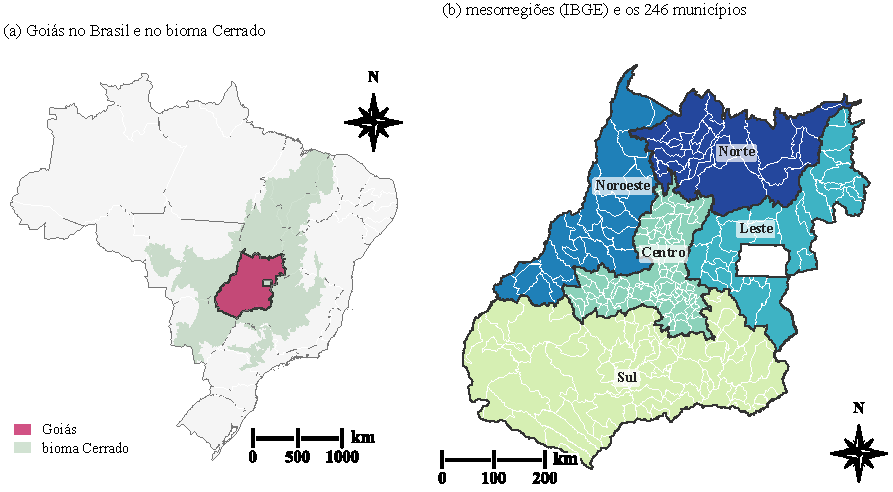
\includegraphics[width=\textwidth]{cap3_localizacao.pdf}
\fontefig{elaboração própria a partir das malhas do IBGE obtidas pelo pacote
\texttt{geobr}: mesorregiões de 2017 --- a mesma malha que a análise emprega
(decisão D6) ---, municípios e estados de 2020, biomas de 2019. Projeção
Policônica do Brasil (SIRGAS 2000, EPSG:5880); os dois painéis estão em
escalas diferentes, cada um com a sua régua. O preenchimento das
mesorregiões segue a ordenação por latitude média dos pixels de conversão da
Tabela~\ref{tab:mesorregioes} --- do Sul (mais claro) ao Norte (mais
escuro) ---, e não a nomenclatura. O vazio a leste do Centro Goiano é o
Distrito Federal, que não integra o estado.}
\end{figure}

\section{Fontes de dados}
\label{sec:met-fontes}

Todas as fontes são públicas e foram coletadas por rotinas automatizadas,
com cache local dos arquivos brutos, de modo que qualquer número do trabalho
possa ser reconstruído a partir do dado original. A
Quadro~\ref{quadro:fontes} resume fonte, cobertura e papel na análise.

A espinha dorsal é a série anual de uso e cobertura da terra do
\citeonline{MapBiomas2025}, em sua Coleção 10.1. A ela somam-se os dados de
pesquisa e registro administrativo do \citeonline{IBGE_SIDRA}, o crédito
rural do \citeonline{BACEN_SICOR}, o índice de desenvolvimento municipal da
\citeonline{FIRJAN_IFDM}, o mapa de aptidão agrícola da
\citeonline{Embrapa_Aptidao}, o cadastro de unidades armazenadoras da
\citeonline{CONAB_Armazenagem}, o monitoramento de desmatamento do
\citeonline{INPE_PRODES} --- usado como aferição externa, e não como insumo
---, o Atlas do Desenvolvimento Humano \cite{IPEA_IDHM} e as malhas
territoriais oficiais obtidas pelo pacote \emph{geobr}
\cite{Pereira2019geobr}.

As siglas nela empregadas designam, pela ordem: o Sistema IBGE de Recuperação
Automática (SIDRA), portal pelo qual se acessam as pesquisas do Instituto
Brasileiro de Geografia e Estatística (IBGE) --- entre elas a Produção
Agrícola Municipal (PAM), a Pesquisa da Pecuária Municipal (PPM), as Contas
Regionais, de onde vêm o Produto Interno Bruto (PIB) e o Valor Adicionado
municipais, o Índice Nacional de Preços ao Consumidor Amplo (IPCA) e o Censo
Agropecuário; o Sistema de Operações do Crédito Rural e do Proagro (SICOR),
do Banco Central do Brasil (BACEN); o Índice de Desenvolvimento Humano
Municipal (IDH-M), publicado pelo Instituto de Pesquisa Econômica Aplicada
(IPEA); a plataforma Trase, iniciativa de rastreamento de cadeias de
\emph{commodities}; a Empresa Brasileira de Pesquisa Agropecuária (Embrapa);
e o PRODES, sistema de monitoramento do desmatamento por satélite do
Instituto Nacional de Pesquisas Espaciais (INPE).

\begin{quadro}[htb]
\centering
\caption[Fontes de dados: cobertura e papel na análise]{Fontes de dados: cobertura temporal e papel na análise.}
\label{quadro:fontes}
\small
\begin{tabular}{p{3.6cm}p{2.4cm}p{7.6cm}}
\toprule
\textbf{Fonte} & \textbf{Cobertura} & \textbf{Papel na análise} \\
\midrule
MapBiomas, Coleção 10.1 (raster, 30~m) & 1985--2024, anual &
Uso e cobertura da terra: estoques por classe, matrizes de transição
pixel a pixel, centros de massa, idade da pastagem. É a espinha dorsal
do trabalho \\
\addlinespace
IBGE/SIDRA --- PAM (tabelas 1612, 1613 e 839) & 1985--2024 &
Área plantada, área colhida, produção e rendimento das lavouras; milho de
1ª e 2ª safras (2003--2024) \\
\addlinespace
IBGE/SIDRA --- PPM (tabelas 3939, 74 e 94) & 1985--2024 &
Efetivo de rebanhos (bovinos e demais), leite e ovos \\
\addlinespace
IBGE/SIDRA --- Contas Regionais (tabela 5938) & 1999--2021 &
PIB municipal e Valor Adicionado por setor \\
\addlinespace
IBGE/SIDRA --- tabelas 6579 e 1737 & 2001--2024; mensal &
População residente; IPCA (deflator) \\
\addlinespace
IBGE/SIDRA --- Censo Agropecuário 2017 & 2017 (transversal) &
Plantio direto, uso de calcário, orientação técnica --- variáveis de
manejo indisponíveis em série \\
\addlinespace
SICOR/BACEN & 2013--2026 &
Crédito rural por município, finalidade e produto \\
\addlinespace
IPEA --- IDH-M & 1991, 2000, 2010 &
Desenvolvimento humano municipal; série descontinuada após 2010 \\
\addlinespace
Trase & 2004--2020 &
Cadeia produtiva da soja e da carne bovina, com separação explícita entre
volume exportado e produção \\
\addlinespace
Embrapa --- aptidão agrícola & estática &
Exposição física exógena (gradiente edafoclimático) nos desenhos de
interação \\
\addlinespace
PRODES/INPE & 2001--2024 &
Validação externa das séries de supressão de vegetação \\
\bottomrule
\end{tabular}
\fontefig{elaboração própria.}
\end{quadro}

Duas observações sobre as variáveis monetárias. Todo valor em reais --- PIB,
Valor Adicionado, crédito --- é deflacionado para reais de dezembro de 2024
pelo IPCA acumulado, construído como número-índice a partir da série mensal e
avaliado em dezembro de cada ano. E as variáveis monetárias anteriores ao
Plano Real foram excluídas da coleta em vez de convertidas: a conversão entre
Cruzeiro, Cruzado, Cruzado Novo e Cruzeiro Real introduziria erro de medida em
séries usadas como regressores. Por isso o valor da produção da PAM e a série
de leite em valor não entram no painel, embora as quantidades físicas
correspondentes entrem.

\section{Unidades de análise: municípios e Áreas Mínimas Comparáveis}
\label{sec:met-amc}

A malha municipal brasileira não é constante no tempo, e Goiás é um caso
severo: o estado tinha 184 municípios com estatística municipal em 1985 e tem
246 hoje. Dados
de sensoriamento remoto e dados de pesquisa comportam-se de maneiras opostas
diante de uma emancipação: o raster é recortado pelo polígono \emph{atual} em
todos os anos, ao passo que a estatística do IBGE é tabulada pelo município
\emph{como ele existia naquele ano}. Ao juntar as duas fontes pelo código
municipal, compara-se, para um município-pai, a cobertura da terra do
território de hoje contra a produção de um território historicamente maior;
para os municípios-filhos, compara-se cobertura contra dado ausente.

O efeito é grande. Dos 246 municípios, 62 (25\%) só aparecem na estatística
municipal depois de 1985, em ondas de emancipação concentradas em 1989 (27),
1993 (21), 1997 (10) e 2001 (4). O total estadual do rebanho atravessa esses
anos sem descontinuidade --- o gado do filho estava contabilizado no pai ---
mas municípios-pai individuais registram quedas de 50\% a 80\% no ano da
emancipação. Ler essas quedas como dinâmica pecuária seria atribuir a um
fenômeno econômico o que é perda de território. E como as ondas de 1993 e
1997 caem dentro das janelas usadas pelas análises longitudinais, tais quedas
dominariam qualquer estimador de variação nesse período.

A solução adotada (decisão D11) é a agregação em Áreas Mínimas Comparáveis
\cite{Ehrl2017}: cada município-pai é reunido aos seus desmembramentos numa
unidade de território constante ao longo de toda a janela. Aplicada a Goiás
com a concordância de 1980--2010 --- janela que antecede todas as
emancipações do período analisado ---, a agregação reduz os 246 municípios a
\textbf{166 AMCs}, sendo 53 grupos de pai e filhos e 113 unidades que
permanecem idênticas ao município. A validação é direta: o total estadual é
idêntico ao da malha municipal e nenhuma das 166 AMCs estreia depois de
1985.

A agregação obedece a uma regra que vale para qualquer variável derivada:
grandezas \emph{extensivas} (hectares, cabeças, reais) são somadas, e
grandezas \emph{derivadas} (razões, densidades, lotação) são
\emph{recalculadas} a partir das extensivas já somadas --- nunca somadas ou
promediadas diretamente, o que produziria média de razões em lugar de razão
de totais.

Disso resulta uma estratégia de dois trilhos, e usar o trilho errado é erro
metodológico: as AMCs (166 unidades) são a malha de toda análise
longitudinal --- primeiras diferenças, painel com efeitos fixos,
periodização, tendências, deslocamento de centros de massa ---, enquanto a
malha municipal atual (246 unidades) fica reservada às análises transversais
e ao período recente, como o Censo Agropecuário de 2017 e os mapas de um
único ano. O preço, com a aritmética correta: os 133 municípios reunidos nos
53 grupos deixam de ser analisáveis isoladamente nas séries longas, e a malha
perde 80 unidades em relação às 246. É um preço inevitável quando o dado vem
de pesquisa, porque a informação histórica do município-filho não existe
separada --- ela estava no pai.

Duas convenções geodésicas sustentam as medidas, e vale separá-las porque
respondem a perguntas diferentes. Toda operação \emph{geométrica} ---
centroides, distâncias, deslocamentos, recortes zonais --- é feita no sistema
de coordenadas de código EPSG:5880, Sistema de Referência Geocêntrico para as
Américas (SIRGAS 2000) em \textbf{projeção Policônica do Brasil}, que é o
padrão cartográfico brasileiro e a projeção em que saem os mapas deste texto;
o EPSG:4674 aparece apenas quando a leitura pede coordenadas geográficas. A
policônica é projeção de compromisso --- não é conforme nem equivalente ---,
e por isso ela não é usada para medir área. As áreas vêm de outro caminho: o
censo de pixels conta células de 30~m na grade nativa do produto e converte a
contagem em hectares pelo cosseno da latitude média observada de cada
município, sem passar por projeção nenhuma. A malha municipal de referência é
a do IBGE para 2020.

\section{O painel unificado e as primeiras diferenças}
\label{sec:met-painel}

As fontes descritas convergem para uma tabela única, organizada por
município e ano --- $246 \times 40 = 9.840$ linhas e 195 colunas --- que
reúne, para cada observação, os estoques de uso da terra, a produção
agrícola e pecuária, o produto e o valor adicionado, o crédito rural, a
população e as variáveis derivadas. É desse painel, e de sua versão agregada
em AMCs, que sai toda a estimação do trabalho.

A segunda decisão estruturante (D7) é que \textbf{nenhuma associação é
estimada em nível}: todas as variáveis entram em primeira diferença,
$\Delta x_t = x_t - x_{t-1}$. A razão é que quase toda série do painel tem
tendência --- área, produção, produto e população crescem ao longo de quatro
décadas --- e correlacionar níveis entre séries com tendência comum produz
associações altas e vazias. Diferenciar remove a tendência e reformula a
pergunta: em vez de ``municípios com mais crédito têm menos pasto?'', o
modelo responde ``quando o crédito de um município subiu, o pasto dele
recuou?''.

Essa escolha foi objeto de auditoria específica. Muitas variáveis do painel
são internamente relacionadas por construção: área plantada e produção, ou
área e valor adicionado, medem facetas do mesmo fato e apresentam correlação
em nível da ordem de 0,9. Estimar uma sobre a outra em nível não seria uma
associação --- seria uma identidade contábil disfarçada. A primeira
diferença, combinada com os efeitos fixos descritos adiante, desarma esse
vazamento: as mesmas duplas apresentam correlação próxima de zero em variação
\emph{within}. A auditoria de circularidade residual encontrou um único caso
não resolvido pela diferenciação --- o abate bovino, que na fonte é
reconstruído como taxa aplicada ao rebanho e, portanto, é redundante com ele
por definição --- e essa variável foi descartada como evidência. Onde ela
ainda aparece em resultado de pipeline, o coeficiente é declarado identidade
contábil, e não associação estimada.

Duas observações da série perdem-se na montagem do painel de estimação, e
convém dizer por quê antes que os $n$ divirjam aos olhos do leitor: a série
de cobertura tem 40 observações anuais (1985--2024), a primeira diferença
consome a primeira e a defasagem de um ano consome a segunda. Daí as
\textbf{38 diferenças anuais} que aparecem nas regressões, no cálculo de
erros-padrão robustos a autocorrelação e na contagem de realizações
independentes do \emph{shifter} macroeconômico. Quando o texto disser 40, o
objeto é a série descritiva; quando disser 38, é o painel estimado.

\section{Periodização orientada pelos dados}
\label{sec:met-periodizacao}

Narrar quarenta anos exige períodos, e a escolha das fronteiras entre eles é
decisão metodológica, não detalhe de exposição. O trabalho recusou ancorar os
períodos em marcos institucionais escolhidos pelo pesquisador --- a pergunta
``por que 2005 e não 2006?'' não teria resposta formal --- e inverteu a
lógica: as fronteiras são estabelecidas pelos dados, e os marcos
institucionais são classificados \emph{a posteriori} pela força da evidência
que os sustenta.

A regra de decisão foi fixada antes de rodar os testes: um método primário
--- estatística sup-F de Quandt-Andrews \cite{Quandt1960, Andrews1993}, na versão multivariada, aplicada
conjuntamente às variações anuais de vegetação natural, pastagem e
agricultura, com segmentação binária --- e dois métodos de sensibilidade
independentes: o detector sequencial de mudança de regime de Rodionov
(STARS, na sigla inglesa) \cite{Rodionov2004} e a
divergência entre matrizes de transição anuais (Kullback-Leibler e variação
total, com significância por permutação). Uma fronteira só é confirmada
quando o método primário e ao menos um método de sensibilidade convergem;
divergência entre os três seria documentada como sensibilidade ao método, e
não resolvida por escolha.

O procedimento devolveu duas fronteiras robustas --- \textbf{2001}
($F = 62{,}2$) e \textbf{2020} ($F = 21{,}5$) --- e uma terceira, em 1991,
com suporte bem mais fraco ($F = 10{,}3$), não adotada. Daí resultam os três
atos que organizam a narrativa do Capítulo~\ref{cap:resultados}: 1985--2000,
2001--2019 e 2020--2024. Dois pontos merecem registro. Primeiro, o p-valor
do sup-F é bruto, porque muitos anos-candidatos são testados; por isso a
periodização passou por uma verificação de falso positivo, aplicando o mesmo
procedimento a séries de ruído para medir quantas quebras aparecem por acaso.
Segundo, a ausência de quebra também é resultado: o Código Florestal de 2012
não produz quebra empírica em nenhuma das três séries, o que rebaixa seu
estatuto de marco periodizador --- ainda que não diga nada sobre seus
efeitos por outras vias.

A tipologia dos marcos institucionais (A, B ou C) organiza essa assimetria:
marcos com quebra empírica coincidente e mecanismo plausível, marcos com
suporte parcial e marcos de importância discursiva sem suporte empírico
detectável são tratados como categorias distintas ao longo do texto.

\section{Instrumental analítico}
\label{sec:met-instrumental}

Os métodos empregados organizam-se pelas quatro frentes de investigação
enunciadas nos objetivos específicos; a definição operacional de cada métrica
consta do glossário (Apêndice~\ref{ap:glossario}).

\subsection{As três camadas de exigência}
\label{sec:met-camadas}

Os instrumentos obedecem a uma hierarquia. Eles não respondem à mesma
pergunta, e tratá-los como equivalentes seria a origem mais provável de um
excesso de afirmação. O trabalho distingue três camadas, e cada afirmação do
Capítulo~\ref{cap:resultados} declara em qual delas se apoia
(Quadro~\ref{quadro:camadas}).

\begin{quadro}[htb]
\centering
\caption[Camadas de exigência por tipo de desenho]{Camadas de exigência: o que cada desenho consegue responder.}
\label{quadro:camadas}
\small
\begin{tabular}{p{2.6cm}p{5.0cm}p{6.0cm}}
\toprule
\textbf{Camada} & \textbf{Pergunta que responde} & \textbf{Limite} \\
\midrule
Correlação em nível estadual &
Houve coincidência temporal entre as duas séries no estado? &
Poucas observações (de 11 a 39) e nenhum controle por confundidores \\
\addlinespace
Painel com efeitos fixos &
Dentro de cada unidade, a variação de $X$ acompanha a de $Y$ depois de
removidos os choques comuns a todos no mesmo ano? &
Não isola marcos específicos; não controla determinante que varie dentro
da unidade ao longo do tempo \\
\addlinespace
Diferenças em diferenças &
Este marco regulatório teve efeito diferencial em Goiás frente a estados
de controle? &
\textbf{Não identifica neste caso}: os marcos testados são federais, de
modo que não existe grupo não tratado \\
\bottomrule
\end{tabular}
\fontefig{elaboração própria.}
\end{quadro}

A terceira camada exige explicação, porque foi \emph{rebaixada} no curso da
pesquisa e isso altera o que o trabalho pode dizer sobre política. Os quatro
marcos submetidos ao teste --- Plano Real, Lei Kandir, Código Florestal e
Cerrado Manifesto --- são federais: valeram no mesmo dia para o estado
tratado e para os controles do mesmo bioma. Sem grupo não tratado, nem o par
que sobrevive a todos os testes de robustez --- tendências paralelas, estudo
de evento e placebo temporal --- identifica efeito causal. O problema está no
desenho, não na estimação, e nenhum teste adicional o corrige; separar as
hipóteses exigiria variação \emph{dentro} do estado, entre municípios mais e
menos expostos a cada marco, que este desenho não possui. O que o coeficiente
mede é exposição diferencial ao mesmo choque, e é assim que ele é reportado:
como sensibilidade de co-movimento. Os marcos institucionais aparecem no
Capítulo~\ref{cap:resultados} como contexto da periodização, nunca como motor
de um resultado.

\subsection{Padrão espaço-temporal: centros de massa}

A descrição do deslocamento usa o \emph{centro médio} ponderado --- a média
das coordenadas de cada unidade, ponderada pela área da classe ou pelo
efetivo do rebanho ---, calculado ano a ano sobre os centroides das unidades
em coordenadas projetadas (EPSG:5880), com os pesos vindos da contagem de
pixels descrita na Seção~\ref{sec:met-area}. É um
instrumento clássico da estatística espacial descritiva, na linhagem de
\citeonline{Lefever1926}, e não uma construção \emph{ad hoc} (Seção~\ref{sec:ref-centroide}).
Duas peças o acompanham: o \emph{centro mediano}, obtido pelo algoritmo de
\citeonline{Weiszfeld1937}, que minimiza a soma das distâncias e é robusto a
um aglomerado dominante; e a elipse de desvio-padrão \cite{Yuill1971}, que
descreve dispersão e orientação da mancha.

Um centro de massa é uma estatística pontual, e sem margem de erro não há
como distinguir deslocamento real de ruído. A decisão D19 supre isso: cada
deslocamento é acompanhado de um intervalo de confiança de 95\% obtido por
\emph{bootstrap} das AMCs, com reamostragem com reposição e $B = 2000$
replicações. A regra operacional, aplicada em todo o texto: \textbf{um
deslocamento cujo intervalo inclui zero nunca é reportado em quilômetros} ---
descreve-se a variável como ancorada.

\subsection{Mecanismo: transições e painel com efeitos fixos}

O mecanismo por trás do deslocamento é lido em dois instrumentos
complementares. O primeiro é a matriz de transição calculada pixel a pixel
entre pares de anos, e não inferida da diferença entre estoques: só ela
permite dizer que classe deu origem a qual, decompondo cada hectare que
mudou em um fluxo orientado. A matriz primária opera sobre sete grupos de
classes, incluindo o Mosaico de Usos como grupo próprio, pelas razões
expostas na Seção~\ref{sec:met-decisoes}.

O segundo é o modelo de painel com efeitos fixos de dois sentidos, principal
ferramenta de inferência do trabalho (decisão D8):

\begin{equation}
\Delta \mathrm{lulc}_{it} = \alpha_i + \gamma_t + \beta \,\Delta x_{it} + \varepsilon_{it}
\label{eq:2fe}
\end{equation}

\noindent onde $\Delta \mathrm{lulc}_{it}$ é a variação anual do uso da
terra na unidade $i$; $\alpha_i$ é o efeito fixo de unidade, que absorve
tudo o que não muda no tempo naquele lugar --- solo, relevo, distância a
mercados, tradição produtiva --- mesmo que tais atributos não estejam
observados no painel; $\gamma_t$ é o efeito fixo de ano, que absorve os
choques comuns a todas as unidades (preços internacionais, câmbio, crises);
$\Delta x_{it}$ é a variação da explicativa de interesse; e $\varepsilon_{it}$
é o erro, com erros-padrão agrupados por unidade. O estimador compara cada
unidade consigo mesma ao longo do tempo, e não umas com as outras.

A especificação em diferenças não é a do manual, que costuma escrever o
modelo em níveis: é escolha deliberada, coerente com D7, porque o objeto
modelado é a \emph{mudança} do uso da terra. Nela, $\alpha_i$ absorve a
tendência própria de cada unidade e $\gamma_t$, o choque comum às variações
daquele ano.

Os diagnósticos que acompanham o painel são o fator de inflação de variância
(VIF), para multicolinearidade entre as explicativas, e o exame da estrutura
espacial dos resíduos. Este último não é rotina: a autocorrelação espacial
dos resíduos (I de Moran, com significância por permutação) mostrou-se
significativa em 115 dos 140 testes na malha municipal e em 125 dos 140 na
malha de AMC --- a dependência espacial não é, portanto, artefato da unidade
escolhida. O que o painel não explica ainda possui organização geográfica, e
foi isso que levou a dimensão espacial ao desenho da frente seguinte, com
modelos de defasagem espacial (SAR, \emph{spatial autoregressive}) e de erro
espacial (SEM, \emph{spatial error model}), além do diagnóstico local de
aglomeração (LISA, \emph{local indicators of spatial association}), este
último tratado como exploratório por não incorporar correção para testes
múltiplos.

Essa dependência tem consequência direta sobre a inferência do painel, e
convém declará-la: o erro-padrão agrupado por unidade, usado nas
especificações principais, corrige a correlação \emph{dentro} de cada
unidade ao longo do tempo, mas não a correlação \emph{entre} unidades
vizinhas no mesmo ano. O reestimador espacial foi rodado justamente para
medir o tamanho desse resíduo: os parâmetros de defasagem e de erro espacial
situam-se entre $+0{,}35$ e $+0{,}56$, confirmando a dependência, e os
coeficientes de interesse atenuam-se em no máximo 12\% quando ela é
modelada. A dependência espacial é, portanto, real e mensurada, e não
derruba os sinais reportados --- mas as magnitudes do painel devem ser lidas
como limite superior.

Nas séries agregadas no nível estadual, em que o painel não se aplica, a
inferência usa erros-padrão robustos a heterocedasticidade e autocorrelação
(HAC, na receita de \citeonline{NeweyWest1987}, com duas defasagens), porque,
com cerca de 38 observações anuais, o erro-padrão ingênuo subestima a
incerteza --- embora, nesse tamanho de amostra, o próprio teste corrigido
tenha pouco poder, o que protege contra falso positivo e esconde efeitos
reais fracos.

\subsection{Deslocamento: precedência temporal e transbordamento}

O teste da hipótese de deslocamento intra-estadual --- a lavoura do Sul
empurrando o pasto para o Norte --- começa pela correlação cruzada com
defasagens (\emph{lead-lag}),
instrumento descritivo que localiza em que encaixe temporal duas séries
melhor se ajustam e orienta onde aplicar os testes formais. O teste formal
de precedência é o de Granger, cujo nome deve ser lido com rigor: ele mede
\emph{precedência preditiva} --- se o passado de uma série ajuda a prever a
outra --- e não causalidade.

A decisão D16 vem de um erro próprio: um teste de Granger aplicado a séries
integradas fabrica precedência inexistente. O exame formal das ordens de
integração, por triangulação entre os testes de Dickey-Fuller aumentado (ADF)
e de Kwiatkowski-Phillips-Schmidt-Shin (KPSS), revelou que a série de
pastagem do Norte é integrada de ordem dois, I(2) --- nem sua primeira
diferença é estacionária --- enquanto a série de
agricultura do Sul é I(0). Séries de ordens diferentes não podem ser
cointegradas, de modo que não há relação de longo prazo entre os níveis para
o teste detectar, e qualquer ``precedência'' encontrada nessa configuração é
artefato.

Três instrumentos corrigem o problema. O primeiro é o procedimento de
Toda-Yamamoto \cite{TodaYamamoto1995}, que ajusta um modelo vetorial autorregressivo em níveis com
$p + d_{\max}$ defasagens --- $p$ defasagens ótimas mais $d_{\max}$
defasagens extras, iguais à ordem máxima de integração --- e aplica o teste
de Wald apenas às $p$ primeiras, tornando a inferência válida sob
integração. O segundo são os \emph{placebos direcionais}: o mesmo teste é
repetido contra destinos economicamente implausíveis; se o sinal persiste
onde não há mecanismo, ele não é direcionado, e sim co-tendência genérica. O
terceiro é o teste de transbordamento direcional entre vizinhos, executado
em tempo contínuo justamente para não reimportar as fronteiras da
periodização (princípio anticircularidade da decisão D12).

\subsection{Drive comum: desenho \emph{shift-share} e inferência por permutação}

A hipótese de que um mesmo motor macroeconômico atinge diferentemente
lugares diferentes é testada por um desenho de interação do tipo
\emph{shift-share} (ou Bartik): o \emph{shift} é o choque nacional --- a
taxa de câmbio ---, comum a todas as unidades em cada ano; a \emph{share} é
a exposição local, medida por uma característica física exógena, o gradiente
de aptidão edafoclimática. O desfecho da especificação confirmatória é a
\textbf{variação anual do rebanho bovino}; a mesma grade foi rodada também
sobre variação de área de pastagem e de área de agricultura, e a
Seção~\ref{sec:res-perna3} reporta os três. O interesse recai sobre o
coeficiente da interação, isto é, sobre o \emph{gradiente} do efeito, e não
sobre seu nível: com efeito fixo de ano no modelo, o nível do choque comum é
absorvido por construção. A previsão testada é que a depreciação cambial
faça o rebanho crescer \emph{mais onde a aptidão edafoclimática é baixa} ---
a fronteira do Norte --- e menos no núcleo apto do Sul, onde a mesma terra
tem uso alternativo mais rentável em lavoura; o coeficiente esperado da
interação é, portanto, negativo. Essa divisão de trabalho com a literatura é
explícita (Seção~\ref{sec:ref-cambio}).

A inferência exigiu tratamento próprio. Para desenhos \emph{shift-share} com
um único \emph{shifter}, o erro-padrão agrupado é otimista
\cite{Adao2019, Borusyak2022}. O trabalho substituiu-o por
inferência por permutação do \emph{shifter}: a série anual do câmbio é
reembaralhada entre os anos, mantidas fixas as \emph{shares}, a interação e
o coeficiente são recomputados a cada replicação, e o p-valor é a fração de
coeficientes nulos que igualam ou superam o observado em módulo. Duas
variantes foram usadas, e a distinção importa: a permutação livre quebra a
autocorrelação do câmbio e tende a ser otimista; a permutação circular, que
rotaciona a série sobre suas posições, preserva a autocorrelação do choque
macroeconômico e é a versão defensável para uma série serialmente
correlacionada. A bateria completa-se com placebos de desfecho (a mesma
interação sobre variáveis que não deveriam responder, como área urbana e
água), placebo temporal e \emph{jackknife} por ano.

O desenho tem um teto: o \emph{shifter} é uma série nacional, com cerca de 38
realizações, de modo que o poder estatístico é limitado pela dimensão
temporal e não aumenta com o número de unidades espaciais. Nenhuma quantidade
adicional de AMCs resolve isso; a consequência para a leitura dos resultados
está na Seção~\ref{sec:met-limites}.

\subsection{Teto de oferta e formas de distribuição}

A quarta frente examina a hipótese de esgotamento da terra convertível por
decomposição entre componentes de oferta e de demanda e pelo exame da
distribuição da idade da pastagem no momento de sua conversão para a
lavoura. Nesse último ponto, a pergunta é se há um ou dois mecanismos
operando, e ela é respondida por mistura de gaussianas: ajustam-se modelos
de uma e de duas componentes e comparam-se pelo critério de informação
bayesiano (BIC). Aqui, porém, entra uma restrição que o próprio desenho
impõe (decisão D23): como a análise roda sobre o \textbf{censo} de eventos, e
não sobre uma amostra, o $n$ é a população inteira, e qualquer afastamento
ínfimo do modelo de uma componente produz diferença de BIC astronômica. A
magnitude do $\Delta$BIC mede o tamanho de $n$, não a força da evidência, e
por isso ela \emph{não} é usada aqui como critério probatório. O que sustenta
a leitura de duas populações são evidências que não dependem de ajuste ---
as medianas de idade por origem anterior e o contraste entre as frações de
pasto jovem e velho ---, com o ajuste servindo apenas para descrever a forma.
É um teste de \emph{forma} da distribuição, não de nível, e as duas leituras
não são intercambiáveis --- ponto a que a Seção~\ref{sec:met-decisoes}
retorna.

\subsection{Multiplicidade}

Sempre que uma família de testes é executada --- e algumas grades deste
trabalho passam de uma centena ---, a significância bruta deixa de ser
informativa: com corte de 5\%, cerca de cinco em cem resultados aparecem
significativos por acaso. Os resultados de grades exploratórias são, por
isso, reportados sob controle da taxa de falsas descobertas
\cite{BenjaminiHochberg1995}, declarando-se explicitamente quantos testes compõem a
família --- porque o tamanho da família altera o veredito, e um resultado
que sobrevive numa grade pequena pode não sobreviver quando ela é ampliada.

\section{Réguas de robustez}
\label{sec:met-robustez}

Além dos testes internos a cada método, as afirmações centrais passam por
cinco réguas transversais, cada uma respondendo a uma objeção previsível (Quadro~\ref{quadro:reguas}).

\begin{quadro}[htb]
\centering
\caption[Réguas de robustez das afirmações centrais]{Réguas de robustez aplicadas às afirmações centrais.}
\label{quadro:reguas}
\small
\begin{tabular}{p{2.2cm}p{4.6cm}p{6.8cm}}
\toprule
\textbf{Régua} & \textbf{Pergunta} & \textbf{Procedimento} \\
\midrule
Tempo & O achado depende de onde cortamos o tempo? &
Quatro resoluções temporais (decisão D12) e teste de largura de janela móvel \\
\addlinespace
Escala & O achado depende da malha espacial? &
Município $\times$ AMC $\times$ pixel; recálculo sem malha intermediária \\
\addlinespace
Latitude & É efeito próprio da variável ou o gradiente
Sul--Norte? &
Correlação parcial controlando latitude em todo recorte transversal
(decisão D14) \\
\addlinespace
Integração & A precedência estimada é espúria? &
Ordens de integração, Toda-Yamamoto e placebos direcionais (decisão D16) \\
\addlinespace
Incerteza & Qual o intervalo de confiança? &
\emph{Bootstrap} de unidades; nada é reportado como deslocamento se o
intervalo inclui zero (decisão D19) \\
\bottomrule
\end{tabular}
\fontefig{elaboração própria.}
\end{quadro}

A régua temporal é método reutilizável, e não verificação pontual. Resumir
quatro décadas em períodos é inevitável, mas qualquer recorte é uma escolha,
sujeita a três riscos: preferir
inadvertidamente o corte que embeleza o achado; comparar períodos de
durações desiguais; e circularidade, quando se ``descobre'' nos períodos
aquilo que os definiu. A decisão D12 responde aos três com o mesmo remédio:
toda análise por período é executada em quatro resoluções --- a série
contínua ano a ano, os atos, uma grade regular de cinco anos e as décadas
--- e o que se reporta é a \emph{concordância} entre elas. As duas grades
regulares são exógenas às fronteiras dos atos, o que as torna um teste
válido; a série contínua é a verdade de referência, e um achado que não
apareça nela é suspeito de ser artefato de agrupamento. Todas as comparações
entre períodos são anualizadas, sob pena de um período curto parecer menor
apenas por ser curto.

A leitura das discordâncias é padronizada: um achado presente em todas as
réguas é robusto; um achado presente nas réguas finas que se dilui na grossa
indica fenômeno curto no tempo, e a resposta correta é localizá-lo, não
descartá-lo; um achado presente nos atos e ausente das grades exógenas é
rebaixado, por suspeita de ser artefato das fronteiras escolhidas.

A régua de escala foi verificada de forma direta. O centro de massa
calculado sobre os centroides das AMCs assume distribuição uniforme da
classe dentro de cada unidade --- suposição não necessariamente neutra,
já que as unidades do Norte são maiores e mais irregulares que as do Sul.
O mesmo centro foi então recalculado sem nenhuma malha administrativa
intermediária, com cada pixel de 30~m pesando por si. As duas medições
concordam dentro de dois quilômetros para todas as classes, contra
deslocamentos medidos em dezenas de quilômetros: o problema da unidade de
área modificável --- MAUP, na sigla inglesa de \emph{modifiable areal unit
problem}, pelo qual resultados calculados sobre unidades espaciais mudam
quando muda o recorte dessas unidades --- existe no desenho, mas não é
material para esta métrica.

\section{Decisões metodológicas críticas}
\label{sec:met-decisoes}

Esta seção registra quatro decisões que alteraram resultados já obtidos. Elas
constam aqui, e não em nota de rodapé, porque respondem à pergunta legítima
``por que seus números mudaram?'' e porque impedem que a escolha mais simples
seja restabelecida por conveniência --- inclusive pelo próprio autor, no
futuro. O registro completo está no Apêndice~\ref{ap:decisoes}.

\subsection{Censo de pixels em lugar de amostra (D21--D24)}

A idade da pastagem é medida sobre o censo completo das conversões de
pastagem em lavoura no estado --- 44.639.028 eventos ---, e não sobre
amostra: a amostragem original
sorteava pixels sobre o retângulo envolvente de Goiás, e não sobre o polígono
estadual, e confundia num único código ``dado censurado'' com ``busca no
dicionário de classes falhou'', que passaram a ser estados distintos (decisão
D22). Como o censo traz contagens, todo módulo que o consome é explicitamente
ciente de peso (contrato D24), sob pena de o gradiente estimado desaparecer
sem aviso. A troca da amostra pelo censo tem ainda uma consequência
inferencial que vale isolar (D23): com $n$ igual à população, os testes de
hipótese perdem o sentido usual, porque qualquer desvio ínfimo do modelo nulo
gera estatística arbitrariamente grande. Nos módulos que rodam sobre o censo,
portanto, a robustez é buscada na \emph{estabilidade entre recortes} --- o
mesmo padrão reaparecendo em mesorregiões, AMCs e no pixel --- e não em
p-valor ou em diferença de critério de informação (Apêndice~\ref{ap:d21}).

\subsection{A mudança de rótulo do Mosaico de Usos (D25--D26)}

No trecho final da série, parte da conversão de pastagem em agricultura passa
a ser rotulada como classe 21, ``Mosaico de Usos''. Toda medida de agricultura
em janela que alcance 2020--2024 é, por isso, reportada como o intervalo entre
a classe ``Agricultura'' isolada, que subconta, e sua união com o Mosaico, que
superconta: considera-se robusta apenas a conclusão que sobrevive nos dois
extremos, e conclusões que dependam da convenção de classe são declaradas como
tais (decisão D26). A união não é correção, e responde a uma pergunta
diferente e mais grossa --- ``quanta terra saiu de pastagem para lavoura ou uso
misto?''. Onde existe fonte independente do classificador --- área plantada,
rebanho, crédito, valor adicionado ---, é ela que responde, e o intervalo fica
reservado ao que só o sensoriamento remoto mede
(Apêndice~\ref{ap:d25}).

\subsection{Oscilação classificatória entre pastagem e savana}

O fluxo reverso de pastagem para vegetação natural, volumoso nas matrizes de
transição, é dirigido quase inteiramente à formação savânica e é
aproximadamente simétrico ao fluxo de ida --- assinatura de oscilação do
classificador, não de regeneração. Daí uma proibição de leitura adotada em
todo o texto: esse fluxo nunca é narrado como recuperação. As conclusões
centrais não dependem dele, porque se apoiam no fluxo direto de conversão e em
saldos líquidos, ambos robustos a uma oscilação simétrica, que se cancela no
líquido (Apêndice~\ref{ap:oscilacao}).

\subsection{Lotação em cabeças por hectare}

A medida de intensidade da pecuária deixou de ser expressa em Unidade
Animal e passou a ser expressa em cabeças por hectare. A conversão para
Unidade Animal aplica um fator constante ao efetivo do rebanho; sendo
constante, ela cancela em qualquer análise de tendência ou de variação, e,
sendo fixa no tempo, produz um nível não comparável entre 1985 e 2024,
porque o peso médio do animal mudou ao longo do período. Nenhuma análise
inferencial do trabalho utilizava a conversão --- ela apenas era exibida ---
e a medida reportada passou a ser a diretamente medida.

\section{Arquitetura computacional e reprodutibilidade}
\label{sec:met-repro}

O trabalho é implementado como um conjunto de 54 rotinas de coleta e análise
em Python, encadeadas por dependências explícitas, com processamento de
imagens no Google Earth Engine onde a escala exige e processamento local do
cubo de transições onde o custo de nuvem não se justifica. Cada rotina tem
documentação própria, registrando pergunta, dependências, arquivos de saída
e limitações conhecidas; o conjunto é indexado por uma ordem lógica que
descreve o papel de cada peça na construção do argumento
(Apêndice~\ref{ap:pipelines}).

Duas convenções sustentam a rastreabilidade. A primeira é que todo número
exibido --- no texto, nas figuras ou na visualização interativa --- deve ser
rastreável até um arquivo de dados que o produziu, e auditorias periódicas
percorrem os números publicados verificando essa correspondência. A segunda
é que o identificador numérico de cada rotina é permanente: rotinas não são
renumeradas quando a ordem lógica muda, porque o número é referência
cruzada em toda a documentação e apagá-lo apagaria também o registro datado
das correções.

Os produtos de uso direto previstos no mestrado profissional derivam dessa
arquitetura: o repositório de rotinas reprodutíveis sobre dados públicos e a
visualização interativa que torna os achados navegáveis.

\section{O uso de inteligência artificial como instrumento}
\label{sec:met-ia}

Esta pesquisa utilizou assistentes de inteligência artificial de forma
intensiva e sistemática, e a metodologia seria incompleta se omitisse esse
fato. A declaração é de transparência operacional; o sentido formativo dessa
escolha está na apresentação.

O escopo do uso foi a implementação: escrita e depuração de código de coleta
e análise, execução de análises exploratórias, produção de figuras e
visualizações, e auditorias de consistência entre o que os dados dizem e o
que os documentos afirmam. A formulação das perguntas de pesquisa, as
decisões metodológicas e a interpretação dos resultados permanecem do
pesquisador. A distinção não é retórica: as decisões numeradas ao longo
deste capítulo --- e as quatro descritas na
Seção~\ref{sec:met-decisoes} --- são escolhas de desenho, tomadas diante de
alternativas com custos diferentes, e é sobre elas que recai a
responsabilidade autoral.

Um instrumento dessa natureza cobra contrapartida de verificação, e a
pesquisa a organizou em quatro práticas. A primeira é o registro numerado
das decisões metodológicas, com data e justificativa, que permite reconstruir
por que cada escolha foi feita e o que ela substituiu. A segunda é a
rastreabilidade obrigatória descrita na seção anterior. A terceira é a
revisão cruzada: análises produzidas com apoio de um assistente foram
submetidas a revisão por outro, de fornecedor distinto, com verificação
manual dos números pelo pesquisador --- prática que se mostrou necessária,
porque essas revisões acertam diagnósticos estruturais e ao mesmo tempo
produzem números que parecem verificados e não são. A quarta é o registro
das autocorreções: resultados que teriam sido publicados e foram superados
por um teste adicional permanecem documentados, e não removidos.

O limite dessa prestação de contas precisa ser explícito: a verificação recai
sobre o produto --- código, número, figura --- e não sobre o processo que o
gerou. É a mesma relação que um pesquisador mantém com uma biblioteca
estatística cujo código-fonte não inspecionou: a confiança se constrói pela
validação das saídas contra fontes independentes, pela reprodutibilidade e
pela consistência interna, e não pela auditoria do instrumento. As auditorias
descritas na Seção~\ref{sec:met-decisoes} mostram o alcance e a necessidade
dessa disciplina: os defeitos ali registrados foram encontrados por
verificação sistemática --- não pelo instrumento.

\section{Limitações metodológicas}
\label{sec:met-limites}

O desenho desta pesquisa não permite algumas afirmações que seriam
convenientes, e enunciá-las aqui evita que apareçam por omissão no
Capítulo~\ref{cap:resultados}.

\textbf{Não há identificação causal forte para o papel do câmbio.} O
desenho de interação estima o gradiente do efeito, não seu nível, e a
inferência apropriada ao caso --- permutação do \emph{shifter} --- não
sustenta significância aos níveis convencionais. O resultado é corroborante e
não estabelecido. O teto é estrutural: um choque macroeconômico nacional
oferece cerca de 38 realizações independentes, e nenhuma quantidade adicional
de unidades espaciais aumenta esse número.

\textbf{Resultado nulo não é refutação.} Onde o trabalho não encontra o
canal de deslocamento intra-estadual, a afirmação sustentável é que a
assinatura testada não aparece nos dados examinados, com o poder disponível
--- e não que o fenômeno de deslocamento indireto de uso da terra tenha sido
refutado, o que exigiria desenho e escala distintos. A distinção entre ``não
encontrei'' e ``não há'' vale, em particular, quando a variável dependente é
medida com ruído, porque erro de medida no desfecho atenua qualquer
associação em direção a zero. Esta pesquisa encontrou um caso concreto disso:
um resultado nulo aparentemente limpo inverteu-se ao ser recalculado nos
mesmos municípios com desfecho medido por censo em lugar de amostra.

\textbf{A mudança de rótulo do Mosaico impõe intervalos, não pontos.} Toda
medida de agricultura em janela que alcance 2020--2024 é reportada como
intervalo entre limite inferior e superior, e conclusões que dependam da
convenção de classe são declaradas como tais. A demonstração que permitiria
converter o intervalo em correção pontual --- discriminar o artefato de
rotulagem dos sistemas integrados reais --- exigiria comparação com a coleção
anterior do MapBiomas e não foi realizada.

\textbf{Os marcos institucionais não são identificados causalmente.} Pela
razão de desenho exposta na Seção~\ref{sec:met-camadas} --- marcos federais
não deixam grupo não tratado ---, o que se estima é exposição diferencial ao
mesmo choque, e não efeito de política. Nenhuma afirmação do trabalho sobre
legislação ultrapassa esse limite.

\textbf{O terceiro ato é curto.} O período 2020--2024 tem cinco anos, e as
estatísticas calculadas sobre ele têm precisão correspondente. Onde uma
afirmação depende exclusivamente desse período, a fragilidade é declarada.

\textbf{Restrições de cobertura das fontes.} O crédito rural só existe em
série municipal a partir de 2013, de modo que os resultados que o envolvem
descrevem uma janela de cerca de oito anos, e não as quatro décadas. O IDH-M
não é publicado após 2010. O Censo Agropecuário fornece variáveis de manejo
apenas para 2017, em corte transversal. O painel com efeitos fixos controla
o que é fixo no lugar e o que é comum ao ano, mas não um determinante que
varie dentro do município ao longo do tempo e tenha ficado fora do modelo ---
razão pela qual os coeficientes estimados são descritos como associações bem
controladas, e não como efeitos causais.

\chapter{Resultados preliminares}
\label{cap:resultados}

\notaguia{Primeira redação, a partir das Partes 1--3 da visualização (cujos
números foram auditados um a um contra os arquivos de saída) e da Parte~4 do
\texttt{guia\_de\_leitura.md}. As figuras deste capítulo são geradas por
\texttt{qualificacao/fig/gerar\_figuras.py}, que as redesenha na largura da
mancha a partir dos mesmos arquivos de dados que os pipelines gravaram ---
nunca a partir dos PNG de tela de \texttt{outputs/}.}

Este capítulo apresenta os resultados obtidos até a qualificação, em duas
camadas. A primeira descreve o fenômeno bruto: quarenta anos de uso da terra
em Goiás, organizados pelos três atos que a periodização estabeleceu, e o
balanço agregado de para onde os hectares foram. A segunda percorre as quatro
frentes de investigação, na ordem em que uma puxou a seguinte: o padrão
existe? qual é o mecanismo? uma região empurra a outra? e por que a conversão
desacelerou onde desacelerou?

Duas convenções de leitura valem para todo o capítulo. Onde a medida depende
da classe ``Agricultura'' em janela que alcance 2020--2024, o número é
reportado como intervalo entre as duas réguas da decisão D26, e conferido
contra uma fonte que não passa pelo classificador. E onde um deslocamento
tem intervalo de confiança que inclui zero, ele não é reportado em
quilômetros (decisão D19).

\section{Quarenta anos em três atos}
\label{sec:res-atos}

A régua temporal da Seção~\ref{sec:met-periodizacao} devolveu duas fronteiras,
e a Tabela~\ref{tab:quebras} mostra a convergência dos métodos que as
sustentam. A de 2001 é apontada pelo método primário com folga e corroborada
pelos dois métodos de sensibilidade. A de 2020, pelo primário e,
decisivamente, por uma fonte que não passa por classificador algum: a área de
soja plantada que o IBGE recolhe em campo quebra em 2020 sozinha.

\begin{table}[htb]
\centering
\caption[Convergência dos métodos de periodização]{Convergência dos métodos de periodização sobre as duas fronteiras.}
\label{tab:quebras}
\small
\begin{tabular}{lll}
\toprule
\textbf{Método} & \textbf{$\sim$2001} & \textbf{$\sim$2020} \\
\midrule
sup-F multivariado (primário) & $F = 62{,}2$ & $F = 21{,}5$ \\
Rodionov/STARS (sensibilidade) & 2004--2006 & --- \\
Divergência entre matrizes de transição & pico em 2003 & pico em 2019--2022 \\
Soja plantada, IBGE (âncora independente) & --- & quebra em 2020 \\
\bottomrule
\end{tabular}
\fontefig{elaboração própria a partir do MapBiomas Coleção 10.1 (Pipeline~\#29).}
\end{table}

A caracterização global dos atos vem de uma análise de intensidade, com
teste de Kruskal-Wallis: os três atos diferem em taxa de mudança
($H = 20{,}3$; $p < 0{,}001$), num teste único que compara os três períodos
simultaneamente, e não em detecções separadas por fronteira. Esse número
\emph{descreve} o contraste; ele não o valida. As fronteiras foram estimadas
dos mesmos dados, maximizando precisamente a diferença que o teste depois
mede, e o teste supõe independência entre observações que são taxas anuais
autocorrelacionadas. A validação que vale é externa, e vem adiante: a série
de soja da PAM quebra em 2020 por conta própria, sem nada saber desta
partição.

Uma candidata a quarto período, em torno de 2005--2006, foi examinada e não
adotada. Aqui também convém expor a instabilidade em vez de escondê-la: a
significância da quebra depende do ano de corte testado --- $p = 0{,}10$ em
2004, $p = 0{,}046$ em 2005, $p = 0{,}12$ em 2006 ---, e é justamente por a
fronteira não se firmar em nenhum ano específico que ela não foi adotada, e
não porque um único teste tenha dado $p = 0{,}060$.

Uma ressalva acompanha a fronteira de 2020. Recontada a matriz de transições
com o ``Mosaico de Usos'' como grupo próprio --- consequência da decisão
descrita na Seção~\ref{sec:met-decisoes} ---, o pico do indicador de
divergência migrou de 2020 para 2022, e os quatro métodos não apontam mais
exatamente o mesmo ano. A fronteira se sustenta porque a âncora que a define
é a série de campo, imune ao classificador.

\subsection{Ato I: a pastagem como herança (1985--2000)}

O primeiro mapa da série já mostra uma fronteira em movimento, e não um
ponto de partida natural. Em 1985, quase um terço de Goiás já é pastagem ---
legado da ocupação dirigida do Cerrado que começa na década anterior e que a
série não alcança. A instabilidade macroeconômica do período desestimula o
investimento agrícola de prazo longo, e a lavoura permanece onde já estava:
manchas pontuais no sudoeste. O que domina o centro-sul é pasto; o que
resiste no norte e no nordeste, sobretudo no Vão do Paranã, é Cerrado.

\subsection{Ato II: expansão e intensificação (2001--2019)}

O ato começa com a moeda estabilizada e a exportação de grãos já
desonerada. O que é novo vem de fora: a entrada da China na Organização
Mundial do Comércio no fim de 2001, a sistematização do crédito rural a
partir de 2002--2003 e o super-ciclo de preços de commodities. A agricultura
goiana passa de 9,3\% para 16,0\% do território ao longo do período. No
mapa, o sudoeste --- Rio Verde, Jataí, Mineiros --- se converte à lavoura
sobre o pasto. A pastagem atinge seu pico por volta de 2003, perto de
14,8~Mha, e passa a ceder área. A pecuária segue dominante em extensão, mas
a dinâmica econômica passa à soja.

\subsection{Ato III: conversão acelerada sob rótulo ambíguo (2020--2024)}

Este é o ato em que a medida engana. Lida apenas pela classe ``Agricultura''
do satélite, a conversão parece ter parado: no Sul goiano, a taxa anual do
fluxo de pastagem para lavoura cai 88\% em relação ao Ato~II. A área de soja
plantada que o IBGE recolhe em campo cresce 38\% no estado na mesma janela.
Recontada pela régua que soma as duas classes --- a pergunta mais grossa,
robusta à reetiquetagem por construção ---, essa mesma taxa no Sul não cai:
acelera 51\%. O que mudou foi o rótulo, não o território.

O que o pasto perde, a lavoura ganha: o recuo da pastagem quase quadruplica
de velocidade, de 0,07 para 0,27~Mha por ano. A vegetação natural, por sua vez,
não muda de ritmo --- perde, em saldo líquido, cerca de 0,06~Mha por ano
tanto no Ato~II quanto no Ato~III ---, mas passa a ceder ao norte, onde ainda
há Cerrado em pé.
Goiás chega a 2024 com 34,9\% do território em vegetação natural, sem que a
série dê sinal de estabilização até aqui. O que mudou não foi a velocidade
da perda, e sim o seu endereço. A Figura~\ref{fig:cobertura} mostra esse
rearranjo no mapa, nos cinco cortes temporais.

\begin{figure}[htb]
\centering
\caption[Cobertura e uso da terra em cinco cortes, 1985--2024]{Cobertura e uso da terra em Goiás nos cortes de 1985, 1995, 2005,
2015 e 2024, em sete classes.}
\label{fig:cobertura}
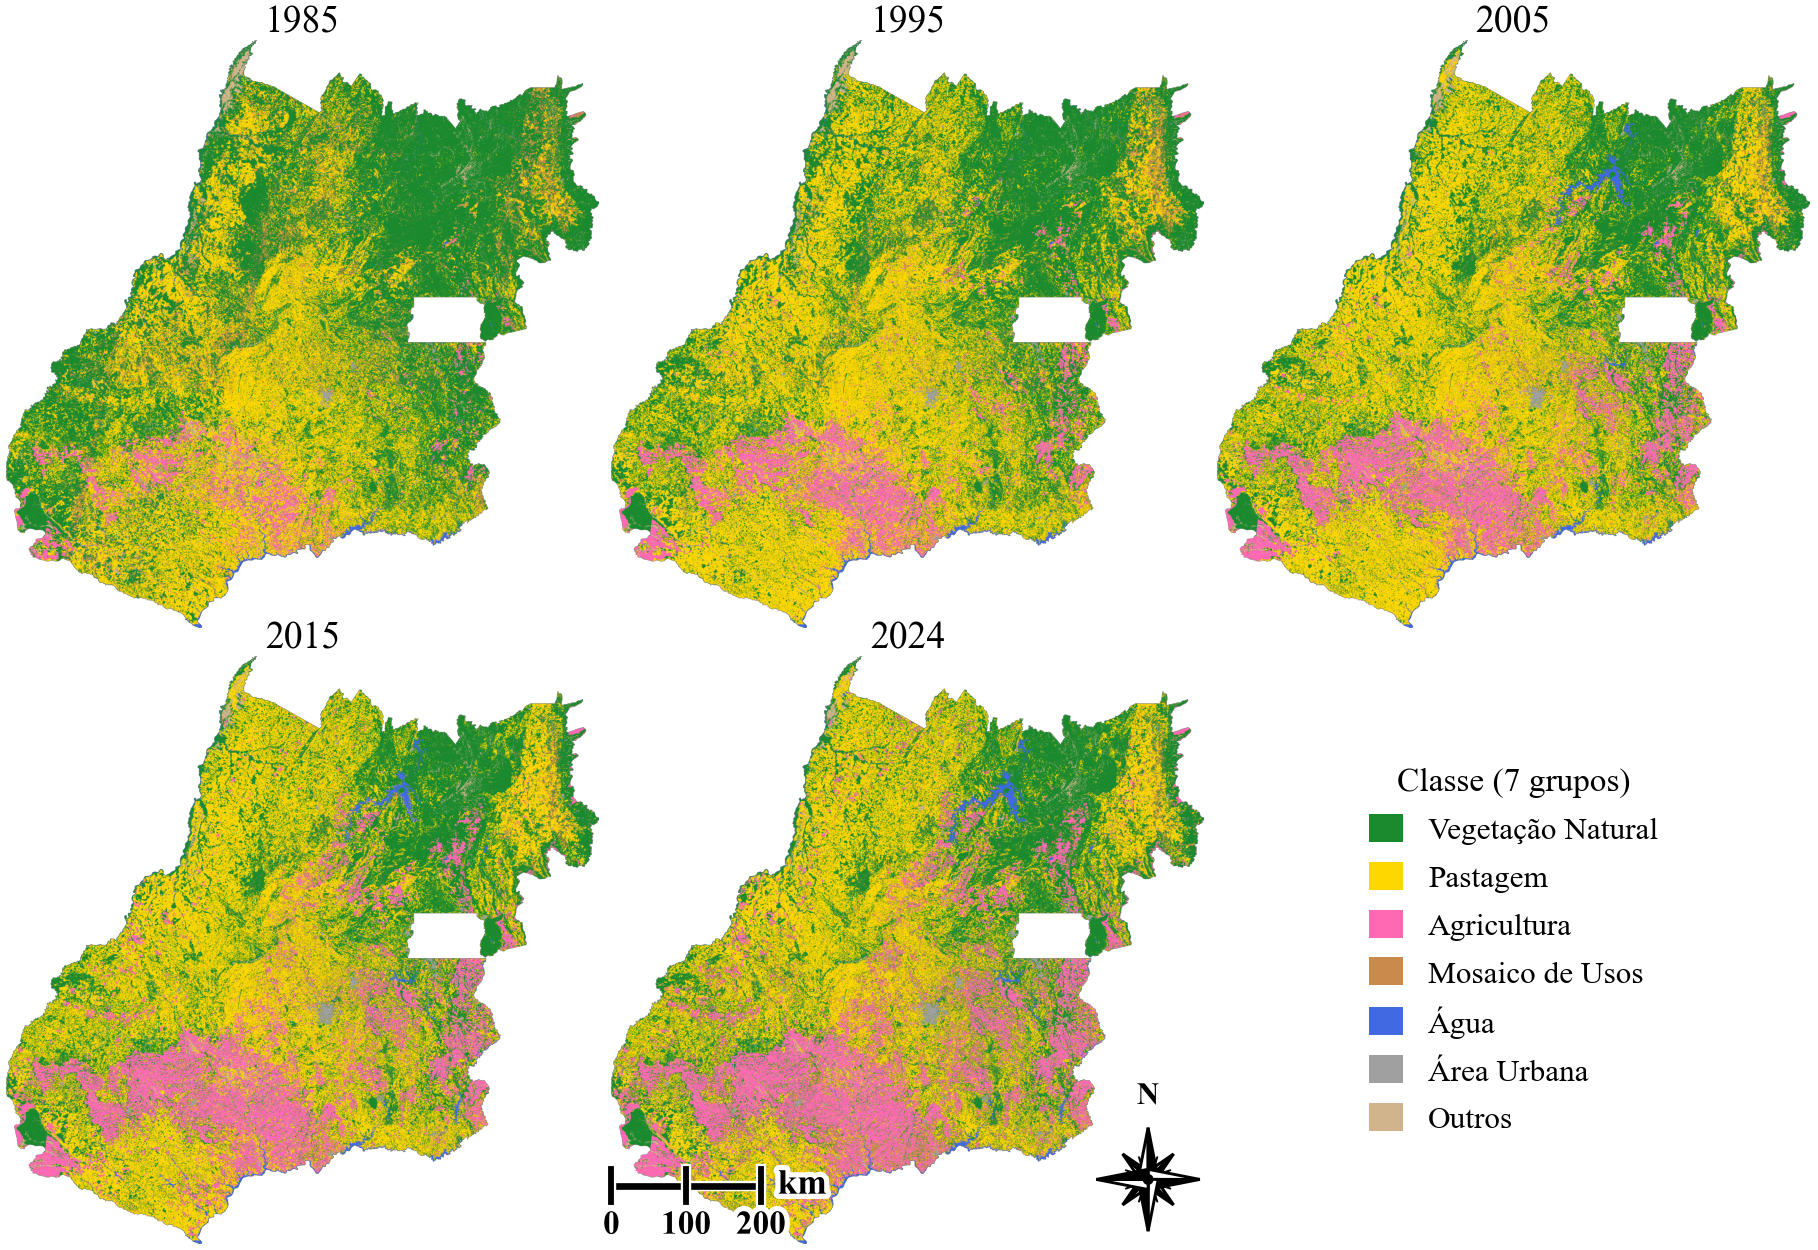
\includegraphics[width=\textwidth]{cap4_painel_cobertura.png}
\fontefig{elaboração própria a partir do MapBiomas Coleção 10.1
(Pipeline~\#10). Os cinco recortes compartilham legenda, projeção, escala e
orientação; por isso a régua e a rosa-dos-ventos aparecem uma única vez, e
valem para todos. Cada pixel mede 387~m. O vazio a leste do centro é o
Distrito Federal, que não integra Goiás e por isso não é classificado.}
\end{figure}

\subsection{O balanço de quarenta anos}

A Tabela~\ref{tab:balanco} resume a transformação agregada, e o saldo líquido
é exatamente o que esconde o caminho dos hectares: duas classes --- pastagem
e Mosaico --- parecem estáveis no saldo e sobem e descem no percurso.

\begin{table}[htb]
\centering
\caption[Balanço agregado de uso e cobertura, 1985--2024]{Balanço agregado de uso e cobertura da terra em Goiás, 1985--2024.}
\label{tab:balanco}
\small
\begin{tabular}{p{3.4cm}p{3.0cm}p{7.2cm}}
\toprule
\textbf{Classe} & \textbf{1985 $\to$ 2024} & \textbf{Leitura} \\
\midrule
Vegetação natural\footnotemark[1] & 17,65 $\to$ 11,88 Mha ($-5{,}8$) &
De 51,9\% a 34,9\% do território \\
\addlinespace
Agricultura & 1,17 $\to$ 5,58 Mha ($\times 4{,}8$) &
A soja cresce $\times 12$ em área (0,37 $\to$ 4,50 Mha) e $\times 13$ em
produção (1,3 $\to$ 17,0 Mt) \\
\addlinespace
Pastagem & 10,98 $\to$ 11,99 Mha ($+1{,}0$) &
Saldo enganoso: a trajetória é em U invertido, com pico próximo de 14,8 Mha
em 2003 \\
\addlinespace
Lotação bovina & 1,45 $\to$ 1,94 cab/ha &
O rebanho cresce 46\% (15,9 $\to$ 23,2 milhões de cabeças) e a área de pasto
apenas 9\%: a pecuária se intensifica \\
\addlinespace
Mosaico de Usos & 3,63 $\to$ 3,59 Mha ($\approx 0$) &
O saldo é nulo, o caminho não: cai de 10,7\% do estado a 6,1\% em 2019 e
volta a 10,5\% em 2024 \\
\bottomrule
\end{tabular}
\fontefig{elaboração própria a partir do painel municipal (Pipeline~\#25),
MapBiomas Coleção 10.1.\\
\textsuperscript{1}~Vegetação natural, nesta tabela, soma formação florestal,
formação savânica, campo nativo \textbf{e campo alagado}. A
Figura~\ref{fig:sankey} adota o agrupamento em sete classes do censo de
pixels, que classifica o campo alagado em ``Outros''; daí a vegetação
natural aparecer lá como 16,96~Mha em 1985, e não 17,65~Mha --- a diferença
é o campo alagado, 0,70~Mha (a subtração dos valores já arredondados dá
0,69). As duas contas são a mesma medida sob duas convenções de classe, e
não uma divergência de dado.}
\end{table}

O cruzamento pixel a pixel entre 1985 e 2024 mostra de onde veio a terra que
cada classe ganhou. Três fluxos desenham a marcha: a conversão de vegetação
natural em pastagem, com 4,10~Mha, é o maior da série --- desmatamento
histórico para pecuária extensiva, concentrado sobretudo nos anos 1980 e
1990; a conversão de pastagem em agricultura, com 2,72~Mha, é a maior
transição entre classes já manejadas, e é ela que permite a expansão da
lavoura sem desmatamento direto; e a conversão direta de vegetação natural
em agricultura, com 1,29~Mha, menor que a rota via pasto, mas existente e
com peso crescente no nordeste após 2010. A pastagem é, portanto, o elo
intermediário da maior parte da entrada em agricultura --- 2,72 dos
4,01~Mha, ou 68\%.

Um quarto fluxo --- 1,00~Mha de vegetação natural para Mosaico de Usos ---
foi deliberadamente mantido fora da conta de conversão antrópica, e a razão
é externa ao próprio dado: incluí-lo faria a razão entre a medida deste
trabalho e a do PRODES/INPE saltar de 1,00 para 1,35, isto é, um terço a
mais de desmatamento do que o sistema oficial registra. Como a classe tem
transição de ida e de volta, tratá-la como perda definitiva superestima.

\begin{figure}[htb]
\centering
\caption[Cruzamento pixel a pixel do uso da terra, 1985--2024]{Cruzamento pixel a pixel do uso da terra entre 1985 e 2024, em sete
classes, com larguras proporcionais à área.}
\label{fig:sankey}
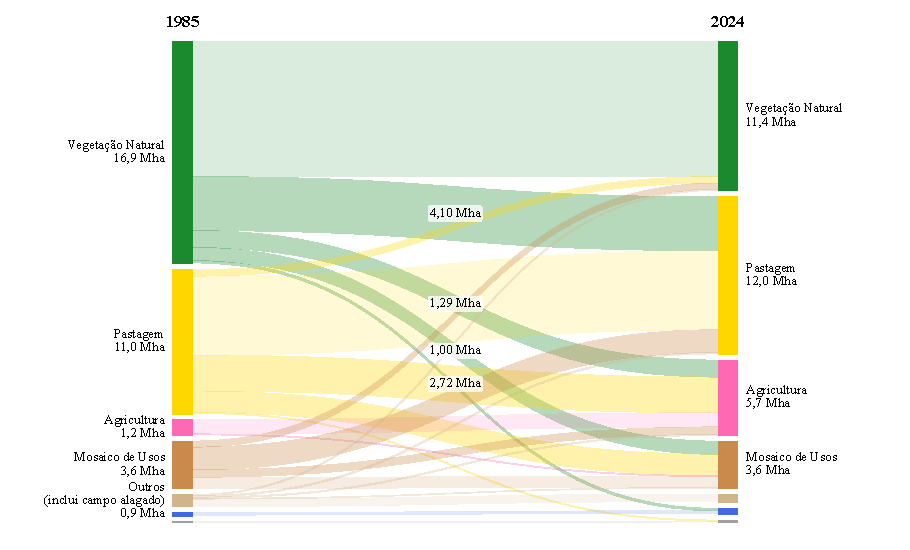
\includegraphics[width=\textwidth]{cap4_sankey.pdf}
\fontefig{elaboração própria a partir da recontagem sobre o cubo do censo de
pixels (Pipeline~\#12B), MapBiomas Coleção 10.1. Fitas inferiores a
0,05~Mha foram omitidas para leitura; os quatro fluxos discutidos no texto
estão rotulados. O agrupamento em sete classes classifica o campo alagado em
``Outros'', e é só por isso que a vegetação natural aparece aqui com
16,96~Mha em 1985 contra os 17,65~Mha da Tabela~\ref{tab:balanco}, que o
conta como natural --- ver a nota daquela tabela.}
\end{figure}

\section{O padrão: a marcha ao norte}
\label{sec:res-perna1}

A primeira frente responde à pergunta mais básica: a fronteira agropecuária
de Goiás se moveu, e para onde? A medida é o centro de massa de cada uso da
terra --- o ponto de equilíbrio geográfico ponderado pela quantidade da
variável ---, acompanhado ano a ano sobre as 166 AMCs. O resultado é
uniforme: tudo marchou ao norte (Tabela~\ref{tab:centros}).

\begin{table}[htb]
\centering
\caption[Deslocamento do centro de massa ao norte, 1985--2024]{Deslocamento do centro de massa ao norte, 1985--2024, com
intervalo de confiança de 95\% por \emph{bootstrap} das AMCs
($B = 2000$).}
\label{tab:centros}
\small
\begin{tabular}{lrll}
\toprule
\textbf{Variável} & \textbf{$\Delta$ Norte} & \textbf{IC 95\%} & \textbf{Veredito} \\
\midrule
Pastagem          & $+77{,}6$ km & $[+54{,}7;\ +98{,}2]$ & robusto \\
Rebanho bovino    & $+66{,}9$ km & $[+47{,}2;\ +84{,}5]$ & robusto \\
Agricultura       & $+65{,}2$ km & $[+43{,}5;\ +94{,}6]$ & robusto \\
Vegetação natural & $+7{,}6$ km  & $[-0{,}5;\ +15{,}6]$  & \textbf{ancorada} \\
\bottomrule
\end{tabular}
\fontefig{elaboração própria (Pipeline~\#32) sobre as 166 AMCs; intervalos de confiança de 95\% por \emph{bootstrap} das AMCs ($B = 2000$).}
\end{table}

Três leituras decorrem da tabela. O deslocamento da pastagem, do rebanho e
da agricultura é grande e está longe de zero. A vegetação natural não
acompanhou: seu intervalo inclui zero, e por isso ela é descrita como
ancorada, e não como tendo andado oito quilômetros --- o que seria ler ruído
como sinal. E existe um gradiente latitudinal persistente: em todos os
quarenta anos, a lavoura permanece cerca de 120 a 130~km ao sul do pasto e do
rebanho --- a expressão métrica dos ``dois Goiáses''.

O tamanho exato desse vão depende da régua: em 2024 ele é de 135~km pela
classe do satélite, 111~km pela régua da união e 122~km pela soja que o IBGE
mede em campo, grande e persistente em qualquer uma das três. A
Figura~\ref{fig:centromassa} traz as trajetórias completas, com a faixa de
confiança de cada série.

\begin{figure}[htb]
\centering
\caption[Centro de massa de quatro camadas]{Centro de massa de quatro camadas: posição em 1985 e 2024 sobre a
malha das AMCs (a) e latitude ano a ano com a faixa de \emph{bootstrap} (b).}
\label{fig:centromassa}
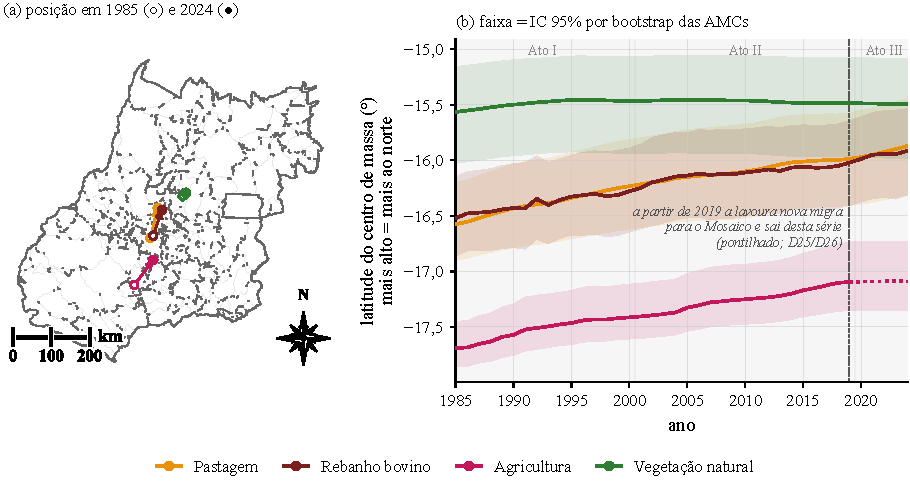
\includegraphics[width=\textwidth]{cap4_centro_massa.pdf}
\fontefig{elaboração própria (Pipeline~\#32) sobre as 166 AMCs; faixa de
confiança de 95\% por \emph{bootstrap} das AMCs ($B = 2000$). Mapa em
projeção Policônica do Brasil (SIRGAS 2000, EPSG:5880), a mesma em que os
centroides são calculados. O mapa mostra o
estado inteiro de propósito: a marcha líquida é de cerca de 80~km num estado
com cerca de 790~km de extensão norte--sul, e um zoom na nuvem de
trajetórias faria um sinal
pequeno, porém robusto, parecer maior do que é. A série da agricultura
aparece \textbf{pontilhada a partir de 2019} porque, dali em diante, parte da
lavoura recém-convertida passa a receber o rótulo ``Mosaico de Usos'' e deixa
de entrar neste centroide (decisões D25 e D26); o achatamento visível no
Ato~III é, em parte não medida, artefato de rótulo.}
\end{figure}

\subsection{Sensibilidade da marcha à régua de medida}

O centroide da agricultura pesa cada região pela área que o satélite rotula
como agricultura --- e, a partir de 2021, parte da conversão recente passa a
receber o rótulo de Mosaico: exatamente a lavoura nova, a da fronteira, deixa
de entrar na conta. A linha achata depois de 2019, e a leitura tentadora
seria que a agricultura parou de subir.

O teste é possível porque nem toda medida do painel passa pelo
classificador. Entre 2019 e 2024, quatro medidas indicam deslocamento ao
norte --- três delas entre 10 e 13~km, a quarta 4,4~km --- e a quinta indica
que nada se moveu. A quinta é precisamente a única cujo rótulo mudou no
período. O rebanho e a soja plantada, medidos em campo, marcham.

Uma segunda evidência fecha o argumento: localizada no mapa, a área que mudou
de rótulo não está espalhada --- o centro dessa massa fica 46~km ao norte
do centro da agricultura visível, e seu crescimento por região acompanha o
da soja do IBGE quase ponto a ponto (correlação de 0,84; 1,52 contra
1,53~milhão de hectares). A conversão que o satélite deixou de nomear está
acontecendo na fronteira. O erro de medida, portanto, aponta contra a tese e
não a favor dela: a régua crua faz a marcha parecer mais fraca do que foi.

Cabe uma distinção que a Seção~\ref{sec:res-perna3} tornará central: dizer
que a lavoura nova está ao norte não é dizer que a lavoura do Sul empurrou
alguém para o norte. A lavoura está subindo junto, não empurrando de trás. O
deslocamento da fronteira agrícola é medido aqui; o de uma região pela outra
foi testado, e não foi encontrado.

A régua da união, porém, não vale para a série longa. Aplicada aos quarenta
anos, ela devolve $-60$~km, isto é, a agricultura andando para o sul --- e o
número não significa o que parece. Em 1985 a classe Mosaico já existia e era
extensa --- 3,63~Mha, 10,7\% do estado ---, situada bem ao norte, e não era
lavoura sob outro nome: era terra de uso misto indiferenciado. Ao longo da
série ela encolhe enquanto a lavoura cresce ao sul, de modo que somar as duas
classes nas duas pontas é comparar objetos diferentes: mede-se sobretudo o
Mosaico antigo se dissolvendo.

A confirmação é espacial: o Mosaico ocupa praticamente a mesma área nas duas
pontas da série, mas as manchas quase não se sobrepõem --- a correlação
espacial entre as células é de apenas 0,15. A de 1985 se dissolveu; a de 2024
surgiu em outro lugar. Por isso a régua da união entra como teto de uma
janela curta, 2019--2024, onde a migração de rótulo de fato ocorre, e nunca
como régua de série longa.

\subsection{Controles de escala e a camada do fogo}

A marcha sobrevive a quatro verificações independentes. Não é artefato de
recorte: refeito pixel a pixel, sem malha administrativa alguma, o
deslocamento reaparece a um ou dois quilômetros do valor original (pastagem
$+79{,}2$ contra $+77{,}6$~km; agricultura $+66{,}9$ contra $+65{,}2$~km).
Não é artefato de agregação de classes: aberta em formações, a vegetação
mostra que a resistência ao norte é da floresta ($+8{,}7$~km, IC
$[+2{,}5; +15{,}1]$), ao passo que o limite do campo nativo se deslocou para
o norte --- direção robusta, magnitude imprecisa, com intervalo largo --- e a
formação savânica tem intervalo que inclui zero. Foi uma autocorreção: o
número médio do agregado escondia comportamentos distintos por dentro. Toda a
marcha vem com barra de erro, pela decisão D19.

E não é deslocamento genérico, o que dois controles estabelecem. A área
urbana não acompanha: ela anda 8~km para o sul (IC $[-19; -1{,}5]$), no
sentido oposto ao da fronteira. E o leite --- pecuária da bacia consolidada
do Sul --- sobe menos da metade do que sobe o rebanho total ($+30$ contra
$+67$~km), de modo que o vão entre os dois centros mais que dobra, de 30~km
em 1985 para 68~km em 2024. Quem marcha é a pecuária de corte na fronteira,
e não o mapa inteiro subindo.

Há ainda uma quinta camada, e ela vai à frente das demais: o centro de massa
do fogo em vegetação natural fica ao norte do centro da conversão em todos
os 39 anos em que as duas séries coexistem --- a de fogo começa um ano
depois da de cobertura ---, com dianteira média de 73~km, sem nunca trocar
de lado. É uma
vanguarda geográfica, e apenas isso: a leitura de que o fogo abriria caminho
foi testada e não se sustenta no tempo --- a liderança temporal desaparece
sob transformação logarítmica, inverte quando se removem os anos de seca de
1985 e 2010, e o teste de precedência agregado é nulo. O fogo marca onde a
fronteira está, não quando ela vai andar.

\section{O mecanismo: duas lógicas simultâneas}
\label{sec:res-perna2}

Se a fronteira inteira marchou, que conversão a moveu, e em que parte do
estado? A marcha é o saldo de duas conversões distintas, e elas não estão no
mesmo lugar. No Sul, a transição dominante é de pastagem para lavoura:
intensificação, terra que troca de função. No Norte, é de vegetação natural
para pastagem: fronteira, terra nova sendo aberta.

A medida que sustenta essa divisão é justamente a que não depende da classe
ambígua, porque nem sua origem nem seu destino passam por ela: a conversão
de vegetação natural em pastagem cai 49\% no Sul Goiano entre os Atos~II e
III e apenas 13\% no Norte, na malha das cinco mesorregiões.

\subsection{A idade da pastagem como medida de intenção}

Saber que o Sul converte pasto em lavoura não diz se aquele pasto era etapa
planejada de um sistema agrícola ou terra parada há duas décadas que enfim se
tornou lucrativa --- duas economias diferentes com o mesmo nome no mapa. A
idade da pastagem no instante da conversão é a aproximação mais próxima da
intenção do produtor que a série permite observar.

O censo de pixels descrito na Seção~\ref{sec:met-decisoes} contabiliza
44,6~milhões de conversões de pastagem para lavoura em Goiás --- 3,8~Mha,
11,2\% do estado. Destas, 16,0~milhões têm idade conhecida; as demais já
eram pastagem em 1985 e têm idade truncada pelo início da série.

A distribuição não é composta por um único tipo de pastagem. O ajuste de
mistura sobre o censo completo separa duas populações: uma jovem e
concentrada ($\mu \approx 4$ anos, $\sigma \approx 1{,}6$ ano, 33\% da
massa) e outra velha e larga ($\mu \approx 16$ anos,
$\sigma \approx 7{,}5$ anos, 67\% da massa), com cauda que alcança os
quarenta anos da série. A forma não tem dois picos visíveis: tem um pico
jovem e um ombro longo --- sendo cerca de cinco vezes mais dispersa que a
primeira, a segunda população produz platô, e não segunda espiga. O que a
estabelece não é a inspeção visual, e sim o fato de uma população única não
dar conta da forma: ajustada sozinha, ela devolve $\mu \approx 12$ anos e
erra as duas pontas, subestimando o pico jovem e a cauda velha.

A leitura de cada grupo apoia-se no que havia no pixel antes de ele virar
pastagem --- e essa leitura não depende de ajuste algum. Separados apenas
pela origem, os eventos se ordenam sozinhos: o pasto que veio de lavoura
volta a ser lavoura com mediana de cinco anos, e o que veio de vegetação
natural dura o dobro, mediana de treze anos. Nas conversões de pasto com até
três anos, 45\% já tinham sido lavoura antes --- lavoura, pasto, lavoura: é
rotação. Nas de pasto com trinta anos ou mais, a lavoura anterior
praticamente desaparece, com 1\%: esse pasto veio de vegetação natural ou de
Mosaico de Usos, em proporções semelhantes --- Cerrado, pasto, lavoura: é
reserva ativada.

Cabe aqui uma ressalva, porque o Mosaico é justamente a classe em que o
classificador não separou usos: metade da origem do pasto velho fica, por
construção, indeterminada entre vegetação natural e uso misto anterior. O
que o dado estabelece com firmeza é o \emph{contraste} entre as duas pontas
--- 45\% contra 1\% de lavoura anterior ---, e não a atribuição de cada
pixel. Na mesma linha, a primeira população é compatível com sistemas de
integração lavoura-pecuária, mas não os comprova: o satélite vê o capim, não
vê se havia gado nele. A Figura~\ref{fig:idade} traz a distribuição de
idades e a decomposição por origem anterior.

\begin{figure}[htb]
\centering
\caption[Idade da pastagem no momento da conversão para lavoura]{Idade da pastagem no momento da conversão para lavoura: a forma da
distribuição contra os ajustes de uma e de duas componentes (a) e a
composição da origem anterior do pixel por idade (b).}
\label{fig:idade}
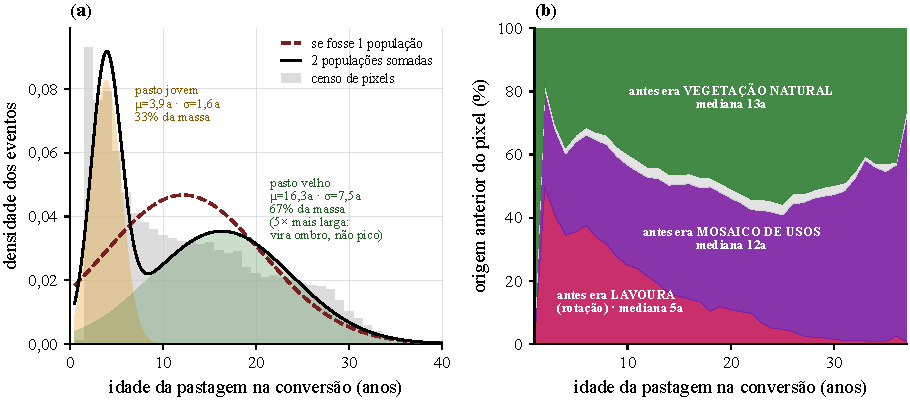
\includegraphics[width=\textwidth]{cap4_idade_pastagem.pdf}
\fontefig{elaboração própria a partir do censo de pixels (Pipeline~\#28C),
MapBiomas Coleção 10.1. Entram apenas os 16,0~milhões de eventos cuja idade é
conhecida; os demais já eram pastagem em 1985 e têm idade truncada pelo
início da série. O painel~(a) mostra por que a segunda população não se lê
por inspeção visual: sendo cerca de cinco vezes mais larga que a primeira,
ela produz um ombro, e não um segundo pico. O painel~(b) recupera a mesma
divisão sem ajustar modelo algum.}
\end{figure}

\subsection{Decomposição regional da idade}

A curva soma quarenta anos de conversões em todo o estado: talvez não haja
duas populações convivendo em lugar algum, e sim regiões ou épocas diferentes
somadas. As duas objeções foram testadas isolando cada recorte.

\textbf{Não são regiões somadas.} Percorridas as cinco mesorregiões, o
desenho é praticamente o mesmo. As cinco são bimodais, e também o são todas
as 166 AMCs na régua imune à mudança de rótulo (na régua estrita, 162 de
164, e as duas exceções falham pelo mesmo lado: peso do grupo jovem baixo
demais para o teste, não ausência de dois grupos). A mesorregião explica
0,5\% da variação da idade.

\textbf{Não são épocas somadas.} Isoladas por período, as duas populações
permanecem: no Ato~II sozinho --- 32,5~milhões de conversões pela régua da
união, o maior bloco da série --- e no Ato~III sozinho, nas cinco
mesorregiões de cada um, em 10 de 10 células de período por região (9 de 10
pela régua estrita). Convém não somar esses 32,5 milhões aos 16,0 milhões
citados acima: aqueles são eventos com idade conhecida na régua estrita,
estes são eventos na régua da união, e as duas contagens medem populações
diferentes. O Ato~I fica fora do teste, e a
razão é instrutiva: ele é unimodal em toda parte e não poderia ser outra
coisa. Uma conversão em 1995 ocorre sobre um pasto que tem, no máximo, dez
anos, porque a série começa em 1985; para observar a conversão de um pasto
de dezesseis anos --- o modo da população velha --- é preciso chegar a 2001.
No primeiro período, a população velha é invisível, não ausente.

Aquele 0,5\% é o que restou da autocorreção mais extensa do trabalho,
apresentada aqui como resultado superado --- a leitura que seria publicada se
um teste específico não tivesse sido feito. A afirmação superada era que o
Sul converteria pasto jovem (mediana de nove anos) e o Norte, pasto velho
(dezesseis anos). O defeito não estava na conta, e sim no que entra nela: a
idade só é medida quando o destino do pixel recebe o rótulo de agricultura e,
no fim da série, parte da conversão passa a ser rotulada como Mosaico. Esses
eventos saem da amostra sem aviso, e não saem por igual no território: saem
mais ao norte. O gradiente era, em boa parte, essa seleção.

Refeita a análise com a pergunta grossa --- imune à reetiquetagem por
construção ---, a amplitude Sul--Norte cai de sete anos para dois, a ordem
das regiões se embaralha e a parcela de variação atribuível à mesorregião
despenca de 3,7\% para 0,5\%. O mesmo ocorre com a forma da distribuição:
na régua estrita, Norte e Noroeste exibem um vale nítido que Sul, Centro e
Leste não têm --- o vale do Noroeste tem profundidade de 42\% ---, e as
cinco regiões se separam em dois blocos. Fechado o viés, a distância entre a
forma do Sul e a do Norte cai de 0,22 para 0,02, e o vale do Noroeste, de
42\% para 6\%.

O que não mudou sob a régua nova foi a coexistência das duas populações. O
achado que sobrevive é, portanto, mais forte do que o que caiu: quanto menos
a região explica, mais universal se mostra a convivência dos dois
mecanismos.

\subsection{Sistema produtivo e crédito como candidatos a explicação}

Descartados os dois eixos óbvios, restavam duas famílias de explicação, cada
uma com uma previsão verificável. A primeira é estrutural: a idade seria
decidida pelo sistema produtivo instalado. O Censo Agropecuário não tem
variável de integração lavoura-pecuária, e o indicador mais próximo
disponível é o plantio direto --- que é prática de conservação de solo, não
de integração com pecuária, ainda que ambas costumem andar juntas na
lavoura tecnificada do Cerrado. A segunda é de fluxo: a idade seria decidida
pelo choque do momento, com o crédito ativando reserva antiga.

Nenhuma das duas explica a idade da pastagem. Para o plantio direto, a
correlação simples confirma a previsão, mas o indicador também se concentra
no Sul; segurando o gradiente espacial (decisão D14), a associação encolhe
cerca de um terço, fica na fronteira da significância sem cruzá-la e não
sobrevive à correção para testes múltiplos. O veredito é
\emph{não estabelecido}, e a distinção importa: um nulo limpo encerraria a
pergunta, um indeterminado não encerra.

Para o crédito rural, a associação é a única que resiste ao controle
espacial, à correção para testes múltiplos e à troca de régua --- na régua
imune ela se fortalece, de $+0{,}22$ para $+0{,}30$. Mas aponta na direção
contrária à esperada: onde o crédito cresceu mais, o pasto convertido é mais
velho, o que é compatível com reserva sendo ativada por dinheiro novo e não
com crédito financiando rotação. Duas ressalvas grandes acompanham o
resultado: ele só existe quando os anos recentes entram --- no recorte até
2019 é praticamente nulo --- e o mecanismo não foi investigado.

A escolha entre girar o capim em três anos ou deixá-lo trinta acontece,
portanto, abaixo da escala que estes dados alcançam: ela não se lê na região,
não se lê no sistema produtivo do município e mal se lê no crédito que chegou
até ele.

\section{O teste do deslocamento e o \emph{drive} comum}
\label{sec:res-perna3}

As duas frentes anteriores entregam dois fatos que, postos lado a lado,
quase escrevem sozinhos uma conclusão: a fronteira inteira subiu ao norte, e
subiu fazendo coisas opostas em cada metade do estado. Somados, sugerem que
o pasto expulso do Sul foi reaparecer no Norte, sobre o Cerrado --- um
deslocamento indireto intra-estadual, com a soja do Sudoeste na origem e a
vegetação do Norte na conta. É a hipótese que mais favorecia a tese inicial
deste trabalho.

Ela tem um problema de lógica antes de ter um problema de dados. Uma
coincidência no espaço não é um mecanismo: dois processos independentes
movidos pela mesma força externa desenham exatamente o mesmo mapa que um
empurrão desenharia. Separar as duas leituras exige procurar uma assinatura
que só o empurrão produz.

\subsection{Efeito de vizinhança e efeito local}

São duas as assinaturas, e ambas são específicas o bastante para poder
falhar --- o que as torna teste, e não ilustração. No tempo, se a lavoura do
Sul empurra, ela precisa mover-se primeiro: a expansão no Sul deve anteceder
o avanço do pasto no Norte, e não apenas acompanhá-lo. No espaço, um empurrão
tem direção: se a lavoura dos vizinhos ao sul cresce e isso expulsa pasto
para cima, o pasto local deve crescer --- um coeficiente $\theta$ que a
hipótese exige seja positivo, com os vizinhos ao norte entrando como placebo.

O teste espacial foi executado em três réguas de medida, cruzadas com duas
janelas e dois desfechos --- doze especificações. \textbf{As doze estimativas
são negativas.} Nenhuma cai na região que a hipótese exige; todas vão na
direção oposta. Quando a lavoura dos vizinhos ao sul cresce, o pasto local
diminui, em vez de aumentar. Não se trata de um p-valor rejeitando uma tese:
trata-se da ausência de um sinal que a hipótese exigia, procurado em doze
recortes e não encontrado em nenhum.

O teste temporal foi executado em vinte e quatro combinações de régua,
janela, desfecho e defasagem. O menor p-valor é 0,078; nenhuma combinação é
significativa. Este nulo tem limites que devem ser declarados: com 38
diferenças anuais, o teste descarta um empurrão forte (poder aproximado de
93\%), mas não um moderado (poder aproximado de 48\%). Sozinho, não
fecharia a questão; somado às doze especificações espaciais, completa o
quadro.

Rodado no sentido inverso, esse mesmo teste temporal produzia um resultado
forte: o Norte anteciparia o Sul, com $p = 0{,}0007$. Se real, ele não
salvaria a hipótese do empurrão --- inverteria a tese inteira. Investigado,
era regressão espúria, e o diagnóstico veio em três passos, nenhum deles ``a
amostra é pequena''. Primeiro, a régua estava errada para o material: o teste
comparava uma série já estabilizada com outra que permanece instável mesmo
depois de convertida em variações anuais --- a montagem clássica que fabrica
precedência. Segundo, o método adequado a séries integradas apaga o resultado
nas duas direções: $p = 0{,}45$ no sentido Norte--Sul e $p = 0{,}25$ no
sentido Sul--Norte. Dizer os dois importa, porque isso também retira qualquer
autorização para afirmar que o Sul lidera: o veredito é \emph{sem líder}, não
``o outro lado venceu''. Terceiro, e mais limpo, os placebos acendem onde não
há mecanismo: o pasto do Norte ``antecede'' o pasto do próprio Sul com
exatamente o mesmo p-valor do resultado original, o que nenhuma economia
explicaria. Uma precedência que aparece em qualquer par de séries suaves não
é mecanismo, é defeito de instrumento.

Deste episódio saiu a regra D16, aplicada retroativamente aos demais
pipelines: nenhum resultado de precedência em série agregada é lido como
causal antes de passar por diagnóstico de estacionariedade, método robusto à
integração e bateria de placebos. A Figura~\ref{fig:espacial} reúne as doze
estimativas do termo de vizinhança.

\begin{figure}[htb]
\centering
\caption[As doze especificações do teste espacial]{As doze especificações do teste espacial do empurrão, com o
intervalo de confiança de cada uma e a zona que a hipótese exigiria.}
\label{fig:espacial}
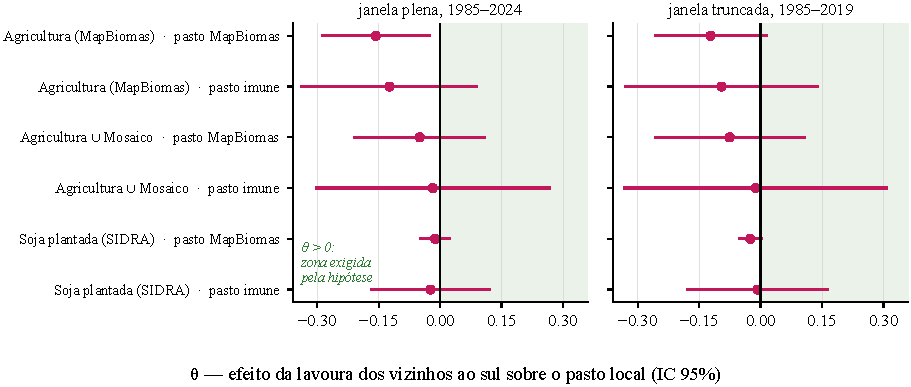
\includegraphics[width=\textwidth]{cap4_teste_espacial.pdf}
\fontefig{elaboração própria (Pipeline~\#49). $\theta$ é o coeficiente do
termo de vizinhança ao sul; as especificações de placebo (vizinhos ao norte)
não estão representadas --- e sobre elas cabe um registro, porque não são
uniformemente nulas: numa das seis células (régua da soja do IBGE, janela
plena) o termo de vizinhança ao norte é significativo a 5\%
($\beta = -0{,}054$; $p = 0{,}032$), justamente onde o termo ao sul
correspondente é nulo. Como o argumento da frente é que um empurrão teria
direção, esse acendimento do placebo direcional enfraquece a premissa e é
mais um motivo para não ler as doze estimativas como um achado.
A faixa sombreada é desenhada porque o resultado é
a \emph{ausência de um sinal que a hipótese exigia} --- e não um p-valor
rejeitando uma tese: as doze estimativas caem do lado oposto ao exigido.}
\end{figure}

O mesmo desenho revela o que ocupa o lugar do empurrão, e o termo precisa ser
preciso: o coeficiente $\theta$ mede o efeito dos vizinhos --- se a lavoura
cresce ao sul, o pasto daqui cresce? --- ao passo que o efeito local mede o
que ocorre dentro do próprio município --- se a lavoura cresce aqui, o pasto
daqui diminui? É a diferença entre empurrão, à distância, e substituição, no
mesmo lugar.

A substituição local é o maior efeito de toda a frente: nas quatro células
medidas em área de satélite o coeficiente vai de $-0{,}52$ a $-1{,}14$, e
$p < 0{,}001$ em cinco das seis células da grade (a exceção é a régua da
soja do IBGE na janela curta, com poucos anos). As duas células restantes,
que regridem sobre a área de soja declarada ao IBGE, ficam em torno de
$-0{,}03$ a $-0{,}07$ --- números que \emph{não} são comparáveis em
magnitude aos primeiros, porque o regressor é outro: um hectare de soja é
subconjunto de um hectare de agricultura. O que se compara entre réguas é o
sinal e a significância, não o tamanho.

O coeficiente dobra quando se amplia a medida --- de $-0{,}52$ na régua
estrita a $-1{,}14$ na que soma agricultura e uso misto. Convém ler esse
salto com cuidado, e não como correção: a régua da união é o teto do
intervalo previsto na decisão D26, não a medida certa. E um coeficiente de
$-1{,}14$ não descreve substituição mais completa --- descreve mais de um
hectare de pasto perdido por hectare de lavoura ganho, o que por definição
excede a substituição e inclui algum fluxo adicional não identificado neste
desenho.

\subsection{O \emph{drive} comum incide sobre um gradiente de aptidão}

Se os dois mecanismos não se comandam, por que marcham juntos? Porque ambos
respondem ao mesmo estímulo externo, e o candidato mais forte é o câmbio
real. O mecanismo é direto: Goiás produz soja e carne para exportação, ambas
cotadas em dólar; quando o real se desvaloriza, a mesma tonelada exportada
rende mais reais ao produtor sem que o preço internacional mude; a
rentabilidade de plantar e de criar sobe, e a procura por terra cresce. O
câmbio não cria fazenda --- ele torna compensador avançar.

Esse impulso, porém, não incide sobre terreno uniforme. O gradiente de
aptidão foi medido por um dado físico que nada sabe sobre quem planta o quê:
o mapa de aptidão agrícola da Embrapa, na escala 1:500.000, com 8.284
polígonos recortados em Goiás. Na escala ordinal da fonte, o gradiente
aparece sozinho --- Sul 4,69, Centro 4,47, Norte 4,17 ---, com correlação de
$-0{,}44$ com a latitude ($-0{,}40$ por Spearman; as três regiões diferem
com $p = 0{,}0002$). Medir o gradiente por um dado físico, e não pelo uso da
terra que se quer explicar, é o que evita a circularidade.

O modelo testa a interação entre os dois, e o desfecho da especificação
confirmatória precisa ser dito com todas as letras: é a \textbf{variação
anual do rebanho bovino}, medida em milhões de cabeças, e não uma medida de
área. A previsão é a de um gradiente invertido em relação ao que o senso
comum sugeriria: sob depreciação cambial o rebanho cresce \emph{mais onde a
aptidão edafoclimática é baixa} --- a fronteira do Norte --- e menos no
núcleo apto do Sul, onde a mesma terra tem uso alternativo mais rentável em
lavoura. O coeficiente esperado da interação é, portanto, negativo.

E aqui entra a ressalva que determina o peso do resultado: sob a inferência
apropriada ao desenho --- permutação do \emph{shifter}, conforme a
Seção~\ref{sec:met-instrumental} ---, o achado é \textbf{corroborante, não
estabelecido}. O coeficiente tem a direção prevista ($\beta = -0{,}033$, com
$R^2$ \emph{within} de 0,001), mas o p-valor honesto fica entre 0,07 e 0,13,
sem cruzar o corte de 5\%. O que sustenta a leitura é a especificidade: cada
teste que deveria sair vazio sai vazio. Os placebos de desfecho são nulos
(área urbana, $p = 0{,}34$; água, $p = 0{,}33$); os placebos no tempo também
($p = 0{,}105$ para a liderança de um ano, $p = 0{,}77$ para a de dois); e o
sinal é estável no \emph{jackknife}, em 38 dos 38 anos.

Três qualificações completam o quadro, e todas as três puxam para baixo o
peso do achado. A primeira é que os desfechos de \emph{área} da mesma grade
são nulos: a interação entre câmbio e aptidão não move a variação de área de
pastagem ($p = 0{,}92$ sem defasagem e $0{,}83$ com um ano), e a interação
entre preço da soja e aptidão não move a variação de área de agricultura
($p = 0{,}77$ e $0{,}60$). Como a narrativa desta seção é sobre procura por
terra, é preciso registrar que o único gradiente com sinal aparece numa
contagem de cabeças, e não na terra. A segunda é de multiplicidade: essa
célula vem de uma grade de 192 testes (quatro exposições, quatro
\emph{drivers}, quatro desfechos, três defasagens), e o próprio exame de
sensibilidade mostrou que ela sobrevive ao controle de falsas descobertas
numa família de 96 testes e não sobrevive numa de 144 --- é, portanto,
sensível ao recorte da família, além de assentar sobre um p agrupado que já
se sabe otimista. A terceira é que o desenho, com efeito fixo de ano, não
poderia mesmo estimar o nível do efeito cambial: ele estima só o gradiente,
e é sobre o gradiente --- não sobre o câmbio como causa --- que a evidência
aqui é corroborante.

Uma precisão sobre esses p-valores, sob pena de se comparar réguas
diferentes: o p do achado é o de permutação, o conservador; os dos placebos
são os agrupados, que a auditoria mostrou serem otimistas. Isso corta a
favor da leitura --- sob a régua conservadora, os placebos ficariam ainda
mais nulos ---, mas não autoriza comparar 0,105 com 0,07--0,13 como se
fossem a mesma medida.

\subsection{Precedência de infraestrutura e crédito}

Uma verificação independente examina se infraestrutura ou crédito puxam a
fronteira. O raciocínio é de simetria: quem puxa costuma estar à frente. Se
silos, bancos ou lavouras puxassem a marcha, seus centros de gravidade
estariam ao norte do pasto e do rebanho; se apenas consolidassem o que já
foi aberto, estariam ao sul.

Nenhuma camada aparece à frente. O centroide do crédito rural fica cerca de
70~km ao sul da pastagem, e esse vão não se fecha --- era 77~km em 2013 e
segue em 69~km em 2024. O da capacidade de armazenagem está ainda mais ao
sul, a cerca de 150~km do pasto, praticamente sobre o núcleo de lavoura do
Sudoeste, a 16~km dele. A cadeia exportadora, medida à parte, co-move sem
liderar. Silo, banco e porto consolidam onde a produção já se instalou. O
resultado é descritivo: diz onde cada camada está, não que ela seja incapaz
de puxar.

\section{A desaceleração e o teto de oferta}
\label{sec:res-perna4}

No Ato~III, o Sul quase deixa de abrir terra nova. A explicação intuitiva
seria o esfriamento do mercado. Ela está errada, e é isso que torna a última
frente interessante: no Ato~III a demanda estava no pico.

Duas precisões mudam a pergunta. A primeira: não foi a lavoura que freou.
Essa leitura seria o artefato de rótulo já desarmado. O que freou é a
abertura de vegetação natural, medida pela conversão de vegetação em
pastagem --- transição cuja origem e cujo destino ficam fora da classe
ambígua. Ela cai 49\% no Sul Goiano e apenas 13\% no Norte, medida na malha
das cinco mesorregiões.

A segunda: não foi o estado que desacelerou, foi o Sul. No agregado de
Goiás, o fluxo \emph{bruto} de conversão de vegetação natural --- a abertura,
antes de descontar o fluxo reverso --- passou de 0,071~Mha por ano no Ato~II
para 0,072 no Ato~III, praticamente o mesmo número. O que mudou foi o
endereço: o fluxo bruto caiu 37\% na região Sul e subiu no Centro e no Norte
--- este na malha de três regiões, e por isso não comparável termo a termo
com os 49\% do parágrafo anterior, que são de outra medida e de outra malha. A marcha não perdeu
velocidade; mudou de lugar. A pergunta desta frente não é, portanto, por que
a fronteira parou --- ela não parou ---, e sim o que a expulsou do Sul.

\subsection{Demanda e oferta na desaceleração do Sul}

Os três sinais de demanda acompanhados desde a frente anterior sobem todos
no Ato~III, e não pouco: o câmbio real vai de 134,5 a 169,0, o preço
recebido pela soja de 104,4 a 186,4 e o crédito rural de Goiás de 14,3 para
24,1 bilhões de reais (série da fonte em reais de 2010, e não na base de
dezembro de 2024 usada no restante do trabalho). A soja efetivamente plantada cresce 38\% na mesma
janela.

O teste que fecha a questão, porém, não é o do estado: é o do próprio Sul,
onde a freada ocorreu. Se o Sul tivesse perdido apetite por terra, teria
parado de converter qualquer terra. Não foi o que houve: no Sul do Ato~III, a
taxa anual de conversão de pastagem em lavoura ou uso misto sobe 51\% em
relação ao Ato~II, e o ritmo de expansão da soja plantada --- os hectares que
o IBGE registra como acréscimo a cada ano --- sobe 244\%, ao mesmo tempo em
que a abertura de Cerrado novo cai pela metade. As duas comparações do
parágrafo anterior e desta, convém frisar, não são a mesma medida: 38\% é o
crescimento do estoque plantado no estado entre as pontas da janela, e 244\%
é a aceleração do acréscimo anual no Sul entre um ato e outro. O Sul não
parou de querer terra. Parou de tirá-la do Cerrado e passou a tirá-la de
pasto já aberto.

A mudança do fluxo entre dois atos separa-se aritmeticamente em duas
parcelas: quanto vem de haver menos Cerrado a converter e quanto vem de
converter a uma taxa diferente o Cerrado que ainda há. A decomposição mostra
que a parcela de estoque é negativa nas três regiões --- em toda parte há
menos Cerrado do que havia, inclusive onde a conversão acelerou --- e que o
que separa as regiões é a parcela residual, que desaba no Sul e sobe no
Centro e no Norte.

O limite dessa figura precisa ser explícito, porque a leitura descuidada dela
diz o contrário do que a evidência sustenta. Apenas 17\% da freada do Sul é,
mecanicamente, ter menos Cerrado; os outros 83\% estão na parcela residual.
E essa parcela \emph{não é demanda}: ela reúne tudo o que não é o tamanho do
estoque --- propensão a converter, atrito de acesso, proteção e a troca de
fonte de terra descrita acima. Se o argumento de oferta dependesse do tamanho
da parcela de estoque, ele seria fraco.

Ele não depende. O argumento se monta por eliminação e por regularidade:
a taxa do Sul caiu enquanto a demanda estava no pico, de modo que o que a
derrubou não é falta de comprador; não é a lei, pelo que se mostra adiante;
a demanda de terra do Sul continuou existindo e foi atendida por pasto já
aberto; e, entre as 164 unidades com dado suficiente para o teste, a taxa de
conversão não cai
sistematicamente com a depleção do estoque ($p = 0{,}48$), nem há saturação
(termo quadrático nulo, $p = 0{,}92$). Quando a taxa é aproximadamente
constante, o fluxo passa a ser ditado pelo tamanho do estoque --- e é esse
resultado, e não a decomposição, que põe a fronteira onde ainda há Cerrado.
A Figura~\ref{fig:fronteira} decompõe a queda entre estoque e taxa.

\begin{figure}[htb]
\centering
\caption[Decomposição da mudança do fluxo entre os Atos II e III]{Decomposição da mudança do fluxo de conversão entre os Atos~II e
III, por região (a), e o estoque convertível remanescente de cada região como
percentual do seu próprio estoque de 1985 (b).}
\label{fig:fronteira}
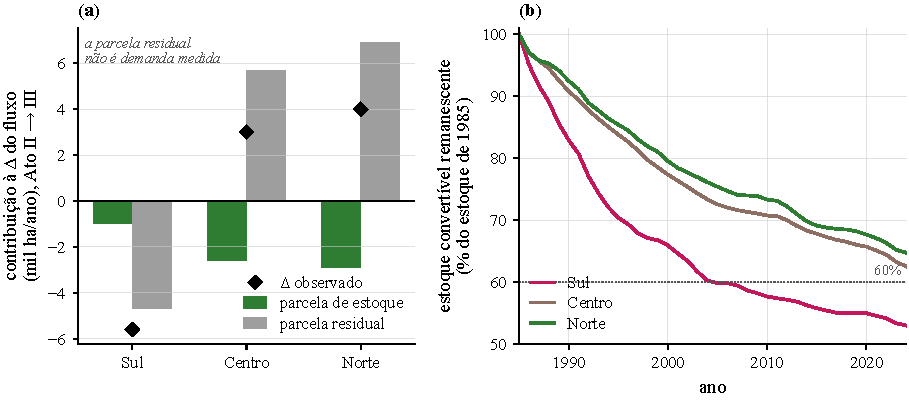
\includegraphics[width=\textwidth]{cap4_fronteira_oferta.pdf}
\fontefig{elaboração própria (Pipeline~\#39). A parcela residual reúne tudo
o que não é o tamanho do estoque --- propensão a converter, atrito de acesso,
proteção e a troca de fonte de terra ---, e \textbf{não é uma medida de
demanda}: lê-la como tal inverteria o sentido do argumento, que se monta por
eliminação e por regularidade, e não pelo tamanho da parcela de estoque.}
\end{figure}

\subsection{O estoque ainda exposto à conversão}

Comparados em hectares, os estoques escondem o que interessa, porque o Sul
sempre foi a menor das três regiões. Postos na mesma régua --- cada região
como percentual do que tinha em 1985 --- as trajetórias se separam. O Sul
desce mais rápido e mais cedo, é o único que cruza os 60\%, e estabiliza a
partir de 2019: perde dois pontos em cinco anos, contra 3,5 do Centro e 3,4
do Norte, que seguem descendo juntos. Não é que o Sul tenha passado a
preservar: é que restou pouco Cerrado em pé a ser suprimido.

Em hectares, restam 6,56~Mha de vegetação natural ainda exposta à conversão
em Goiás, cerca de 60\% do que havia em 1985, e o Norte concentra 44\%
deles. O termo ``convertível'' mede exposição, e não disponibilidade: é o
Cerrado que ainda pode ser perdido, não uma reserva de terra que este
trabalho trate como aproveitável.

A definição adotada --- formação savânica e campo nativo --- não é
arbitrária, e decorre do que a própria depleção mostra: entre 1985 e 2024, a
formação savânica perdeu 38,2\% de sua área e o campo nativo 42,5\%,
enquanto a floresta perdeu 22,8\%. Savana e campo são as classes que a
fronteira de fato consome. O limite da medida é declarado: sem cadastro
ambiental integrado pixel a pixel, o estoque inclui Reserva Legal e Área de
Preservação Permanente (APP) que
na prática não podem ser convertidas, de modo que ele é um \emph{teto} --- a
terra realmente exposta é menor que 6,56~Mha, nunca maior. Um cenário de
sensibilidade descontando 20\% de Reserva Legal foi executado e não altera o
ordenamento entre regiões.

Esse limite merece ser levado às últimas consequências, porque nele mora a
alternativa mais séria à leitura de teto de oferta. O que este trabalho
elimina com dado é a \emph{proteção integral}: unidades de conservação de
uso restrito cobrem parcela pequena do estado, estavam congeladas desde
antes da freada e não explicam o momento em que o Sul desacelerou. Reserva
Legal e APP são outra coisa. Elas incidem dentro de cada propriedade,
ganharam fiscalização efetiva com o Cadastro Ambiental Rural a partir de
2012 --- justamente na janela de interesse --- e tendem a morder mais forte
onde o remanescente já é escasso, porque ali o que sobrou de vegetação
tende a ser precisamente o passivo legal. No Sul depletado, portanto,
``acabou a terra convertível'' e ``o que restou é legalmente inconversível''
produzem a mesma série observada. O cenário de $-20\%$ testado acima
compara regiões entre si e não separa essas duas leituras dentro do Sul;
separá-las exigiria o cadastro ambiental integrado pixel a pixel, que este
trabalho não teve. Fica registrado como limite, e não como questão vencida.

Uma fronteira pode parar por duas razões muito diferentes --- porque a terra
acabou ou porque a lei a barrou --- e as duas produzem o mesmo gráfico
enquanto pedem políticas opostas. Em Goiás, a proteção não estava no caminho
da fronteira. Se o teto fosse institucional, a proteção teria vindo antes da
freada e estaria onde a fronteira vai; não veio, e não está. Dos 6,56~Mha
ainda expostos, 6,35 estão fora de Unidade de Conservação de Proteção
Integral: 97\% pela malha de unidades de conservação e 94,3\% quando a mesma
conta é refeita pixel a pixel, que é a régua mais exigente. A Proteção
Integral cobre menos de 3\% em qualquer região, e congelou: 76\% da que Goiás
tem hoje já existia em 1985 e 89\% já existia em 2000 --- em quarenta anos
ela cresceu 0,12~Mha, contra 4,11~Mha suprimidos do mesmo estoque convertível
(os 10,67~Mha de savana e campo de 1985 reduzidos aos 6,56~Mha de hoje). O
que cresceu nos anos 2000 foi o Uso Sustentável, que admite uso rural e não
veda conversão.

O sentido de ``desprotegido'' aqui é estreito e precisa ser dito: fora da
única categoria que veda a conversão. Não significa livre para desmatar ---
Reserva Legal e APP seguem valendo dentro de cada propriedade e protegem
parte desse mesmo estoque, e é por isso que os 6,56~Mha são um teto. A conta
mede outra coisa: se o instrumento de política que poderia deter a fronteira
de propósito está no caminho dela. Não está --- e o Norte, que guarda 44\%
do que resta, não tem pela frente área protegida que barre a conversão.

\subsection{Custo de carbono e desenvolvimento municipal}

Duas contas fecham a frente, e nenhuma é econômica no sentido usual.

A primeira é de carbono. A conta segue a lógica de diferença de estoque do
IPCC em seu nível mais simples (\emph{Tier}~1): a cada hectare convertido
atribui-se a densidade de carbono da formação que havia ali, e a emissão é a
diferença entre o estoque antes e depois. Duas declarações de escopo são
devidas. A primeira é que a conta cobre apenas a \textbf{biomassa} --- acima
e abaixo do solo ---, e \emph{não} o carbono do solo, que no Cerrado é
parcela grande do estoque total; o número abaixo é, portanto, um piso do
passivo, não o passivo. A segunda é que a faixa reportada não é intervalo de
confiança estatístico: ela vem de rodar a mesma conta sob três conjuntos de
densidades por formação --- baixo, central e alto (decisão D18) ---,
colhidos da literatura de estoques do Cerrado
\cite{Bustamante2012, Grace2006}, das diretrizes do \citeonline{IPCC2006} e,
para a delimitação das fitofisionomias a que cada densidade se aplica, de
\citeonline{RibeiroWalter2008}. Vale registrar que o Cerrado tem razão raiz:parte
aérea alta, de modo que savana e campo estão longe de ser desprezíveis na
conta. Assim precificada, a conversão comprometeu da ordem de
973 milhões de toneladas (Mt) de dióxido de carbono equivalente
(CO\textsubscript{2}e), em faixa de 751 a 1.208 conforme o cenário de
densidade. Duas coisas surpreendem. A primeira é
quem paga: a floresta perde 2,6 vezes menos área que a formação savânica e
ainda assim emite mais (499 contra 458~Mt), porque é cerca de três vezes
mais densa --- o custo de carbono não é proporcional à área. A segunda é
quando se pagou: 80\% do total, 774~Mt, saiu no Ato~I, a 51,6~Mt por ano,
com o Sul como maior emissor do período --- 307~Mt, ou 40\% do ato, a
20,5~Mt por ano. Depois de 2001 o ritmo cai cerca de seis vezes (8,2~Mt por
ano no Ato~II) e a geografia se inverte --- no Ato~III o Sul é o menor
emissor (1,4~Mt/ano) e o Centro o maior (4,6). O centroide da emissão marcha
98~km ao norte, atrás da fronteira. No acumulado dos quarenta anos, note-se,
as três regiões emitem parcelas próximas (Sul 36\%, Norte 32\%, Centro
32\%): o que distingue o Sul não é o total, é o fato de ele ter emitido cedo.

A segunda conta é humana, e exige cuidado para não dizer mais do que mede.
Entre 2013 e 2021, a fronteira norte quase dobrou a área cultivada
($+93\%$, contra $+14\%$ no Sul). O desenvolvimento municipal, medido pelo
Índice FIRJAN de Desenvolvimento Municipal (IFDM) --- indicador composto de
emprego e renda, educação e saúde, publicado pela Federação das Indústrias do
Estado do Rio de Janeiro ---, subiu em toda parte no período --- em Goiás, de
0,49 a 0,63 --- mas
subiu no Norte na mesma medida que no Sul, e o Norte terminou onde começou
em relação a ele: o vão permanece intacto ($-0{,}083$ em 2023, IC 95\%
$[-0{,}108; -0{,}058]$, contra $-0{,}092$ em 2013). Quase dobrar a área não
comprou desenvolvimento adicional nem aproximou a fronteira do núcleo. Num
painel de efeitos fixos dentro do município, dobrar a área vale 0,008 ponto
de IFDM, contra os cerca de 0,15 que o índice subiu na década. A leitura é
associativa, com o gradiente espacial controlado, e não causal.

Vários dos resultados centrais deste capítulo são nulos, e um nulo mal
enunciado converte-se numa afirmação maior do que a evidência sustenta; o
alcance e os limites de cada um estão consolidados na
Seção~\ref{sec:disc-limites}. Os resultados que teriam sido publicados se um
teste específico não tivesse sido feito, e a distância entre cada versão
superada e a que ficou no lugar, estão no Apêndice~\ref{ap:superados}.

\chapter{Discussão}
\label{cap:discussao}

\notaguia{Primeira redação, a partir do quadro de posicionamento do
Capítulo~\ref{cap:referencial}, dos resultados do
Capítulo~\ref{cap:resultados} e de
\texttt{Textos/referencia/referencial\_marcha.md}. Vale para este capítulo a
mesma restrição bibliográfica declarada no Capítulo~\ref{cap:referencial}:
autores mencionados sem vínculo em \texttt{ref/referencias.bib} aguardam
conferência de autoria e edição.}

Os resultados do capítulo anterior descrevem um estado que se reorganizou
sem mudar de tamanho: a mesma superfície, ocupada de outro modo, com a
conversão migrando do Sul para o Norte ao longo de quatro décadas. Este
capítulo pergunta o que essa descrição acrescenta ao que já se sabia, o que
ela implica para o Cerrado que resta e o que, do que foi apresentado,
sustenta peso de conclusão e o que apenas sustenta peso de indício.

A ordem segue a do referencial: o posicionamento na literatura --- a fronteira
e a renda da terra, o deslocamento indireto, o motor macroeconômico e o
espelho do Cerrado ---, as implicações ambientais e de política, e a
consolidação do alcance e dos limites, que até aqui apareceram dispersos junto
de cada resultado.

\section{A fronteira, a renda da terra e uma transição truncada}
\label{sec:disc-fronteira}

O achado que melhor dialoga com o referencial não é a marcha em si, e sim a
sua forma: camadas que sobem juntas sem que o vão entre elas se feche em
quatro décadas, e com magnitudes de deslocamento próximas. É a assinatura que o modelo de localização de von Thünen prevê
quando a ordenação por renda da terra é estável e o que se desloca é o
conjunto: não uma linha que avança, mas um arranjo que se translada sobre um
gradiente.

A contribuição de método por trás desse resultado vale enunciar, porque a
alternativa era circular. A ordenação ricardiana costuma ser \emph{assumida}
e depois ilustrada pelo próprio uso da terra que se quer explicar; aqui o
gradiente, medido por um dado físico exógeno, reproduziu sozinho a ordenação
Sul--Centro--Norte (Seção~\ref{sec:res-perna3}). A premissa do arcabouço
tornou-se uma medida independente dele.

Quanto à síntese de \citeonline{Angelsen2007}, a previsão era que gradiente
espacial e pico temporal fossem faces do mesmo processo. É o que se observa:
as duas aparecem simultaneamente e em lugares diferentes do mesmo estado ---
o gradiente no eixo Sul--Norte, o pico na região que abriu primeiro. Poder
observá-las sob um único desenho analítico, na mesma malha e com o mesmo
classificador, é o que o recorte estadual oferece e o recorte de bioma não.

Já a transição florestal tem uma das duas metades de sua previsão contrariada.
O Sul goiano cumpre a primeira --- estoque reduzido, taxa de conversão
cadente, estabilização a partir de 2019 --- e não cumpre a segunda: não há
regeneração líquida. A estabilização é depleção, não recuperação: perde-se
pouco porque restou pouco a perder, não porque a vegetação esteja voltando.

Essa leitura é o que sobra depois de uma verificação específica. Nas matrizes
de transição existe um fluxo reverso
volumoso de pastagem para vegetação natural, que seria a evidência natural de
regeneração. Examinado em classe bruta, ele se mostrou dirigido quase
inteiramente à formação savânica e aproximadamente simétrico em relação ao
fluxo de ida --- assinatura de oscilação do classificador na borda entre
pasto e cerrado, não de recuperação
(Seção~\ref{sec:met-decisoes}). O componente real de regeneração é
minoritário, restrito à formação florestal, e só se acumula em horizontes
longos. A implicação para o referencial é direta: o caso goiano sugere que a
fase tardia da transição florestal pode consistir apenas em exaustão da
oferta, sem a virada de sinal que o modelo associa a ela --- uma transição
truncada. Se isso é peculiaridade do Cerrado, do período ou do estado, este
desenho não decide; mas registra que a estabilização observada não autoriza a
leitura otimista que o arcabouço sugere.

Quanto à tradição brasileira, a distinção de \citeonline{Martins1996} entre
frente de expansão e frente pioneira dá o vocabulário mais preciso disponível
para os ``dois Goiáses'', com uma calibragem: as categorias de Martins são
sociológicas --- relações de trabalho, formas de propriedade, grau de mediação
capitalista da ocupação --- e o que este trabalho mede são coberturas do solo
e agregados econômicos municipais. A correspondência é analógica e serve para
nomear o contraste; não constitui teste da tese de Martins, e nada nos dados
aqui reunidos poderia constituí-lo. O mesmo vale para a leitura geopolítica de
Becker: informa a interpretação do Norte goiano como território em disputa,
mas o desenho não observa Estado, projeto ou agente.

\section{O deslocamento indireto: um nulo onde havia razão para esperar efeito}
\label{sec:disc-iluc}

O resultado de maior consequência para o posicionamento é um nulo, e a forma
de enunciá-lo determina se ele contribui ou se apenas confunde.

O canal definido na Seção~\ref{sec:ref-iluc} --- empurrão de curta distância
e curta defasagem, de uma metade do estado sobre a outra --- não apresentou,
em trinta e seis recortes, a assinatura que exigiria
(Seção~\ref{sec:res-perna3}). Como a Seção~\ref{sec:ref-iluc} registrou, esse
nulo não é previsão cumprida: havia razão teórica para esperar o efeito, e o
precedente mais próximo, no mesmo nível municipal, encontrou-o na Amazônia.
Como diferem a região, o desfecho medido e a forma da ligação espacial, a
divergência em relação a \citeonline{Arima2011} delimita o que resta comparar
em vez de estabelecer contradição.

Duas precisões impedem que essa leitura cresça além do que sustenta. A
primeira já foi enunciada e se repete aqui porque é a mais fácil de perder na
citação de terceiros: o trabalho não refuta o deslocamento indireto de uso da
terra. Ausência da assinatura testada não é ausência do fenômeno, e ficam
expressamente fora do alcance do teste um deslocamento de longo alcance que
pule os vizinhos, um de defasagem longa, um efeito temporal moderado que o
poder do teste não alcança e qualquer canal que atravesse a divisa do estado.
Ficam descartados, com margem confortável, um empurrão local visível na série
e um empurrão temporal forte.
A segunda é que o veredito temporal é \emph{sem líder}, e não ``o Sul não
lidera, logo o Norte lidera''. O método adequado a séries integradas zera a
precedência nas duas direções, e o episódio que produziu essa correção ---
uma precedência forte no sentido inverso, que se revelou artefato de
integração --- está registrado como resultado superado justamente para que a
simetria do veredito fique visível.

O que ocupa o lugar do empurrão é substancial e positivo. O maior coeficiente
de toda a frente é o da substituição local: dentro do próprio município,
quando a lavoura cresce, o pasto recua. É o desfecho observado da disputa por
terra que \citeonline{Cohn2014} projetam em modelo: no Sul goiano ela aparece
resolvida, e resolvida a favor da lavoura.
A literatura de intensificação e a de
deslocamento costumam ser mobilizadas em conjunto, como se o mesmo dado
sustentasse as duas; aqui elas se separam empiricamente: o mecanismo local
aparece em quase toda especificação, e o mecanismo à distância não aparece em
nenhuma.

Um detalhe do resultado espacial pede prudência interpretativa. As doze
estimativas são todas negativas --- isto é, quando a lavoura dos vizinhos ao
sul cresce, o pasto local diminui ---, e onze delas não são significativas;
a décima segunda é significativa, mas no sentido \emph{oposto} ao que a
hipótese de empurrão exigia. A leitura
tentadora seria transformar isso num achado sobre transbordamento invertido.
Ela não se sustenta com este desenho: o mais que se pode dizer é que a
substituição local tem alguma expressão espacial --- municípios vizinhos
compartilham a mesma dinâmica de troca de pasto por lavoura --- e que isso é
o oposto do que a hipótese do empurrão exigia. O sinal é informativo por
excluir a hipótese testada, não por estabelecer outra em seu lugar.

\section{O motor comum e a divisão de trabalho com a literatura}
\label{sec:disc-drive}

Se as duas metades do estado não se comandam, resta explicar por que marcham
juntas, e a resposta proposta --- resposta coordenada a um estímulo externo
comum, incidindo sobre um gradiente de aptidão --- precisa ser apresentada
com o peso que a evidência lhe dá, que não é o peso de uma demonstração.

A divisão de trabalho com a literatura, enunciada na
Seção~\ref{sec:ref-cambio}, é o que torna a leitura defensável: o nível
causal do canal cambial vem de \citeonline{Richards2012}, em escala nacional
e continental, e o que esta pesquisa estima é apenas a geografia desse
efeito dentro do estado.

Sobre esse gradiente, o veredito é corroborante e não estabelecido. O
coeficiente tem a direção prevista, mas o p-valor apropriado ao desenho ---
permutação do \emph{shifter}, que substitui um erro-padrão agrupado
reconhecidamente otimista para desenhos com um único choque --- fica entre
0,07 e 0,13, sem cruzar o corte convencional. Os p-valores agrupados de 0,026
e 0,031, produzidos pelo desenho anterior, não devem ser citados como
significância. O que sustenta a leitura não é
a significância, e sim a especificidade: os placebos de desfecho saem vazios,
os placebos no tempo saem vazios e o sinal é estável no \emph{jackknife} por
ano. Um padrão que aparece só onde deveria aparecer é evidência de tipo
diferente da que um p-valor fornece, e menos conclusiva do que ela.

O teto dessa frente é estrutural, e convém dizer o que ele exigiria para ser
levantado. Um choque
macroeconômico nacional oferece da ordem de 38 realizações independentes, e
nenhuma quantidade adicional de unidades espaciais aumenta esse número: o
poder é limitado pela dimensão temporal. Levantar o teto exigiria um
\emph{shifter} com variação transversal própria --- exposição diferencial a
preços por produto, por exemplo, em vez de uma única série nacional --- ou
uma janela temporal maior, ou um painel de vários estados que multiplicasse
as realizações do choque. São desenhos distintos, não robustez adicional
sobre este.

Segue disso uma delimitação que precisa acompanhar qualquer citação deste
resultado: o que a pesquisa estabelece é o \emph{mecanismo} --- reorganização
sob força comum, e não empurrão entre regiões ---, e não a identidade da
força. O câmbio é o candidato mais forte e permanece candidato. Qual variável
exatamente aciona o gatilho, o dado estadual não tem como cravar, porque
preço internacional, câmbio, crédito e expectativa de renda movem-se juntos e
são absorvidos pelo mesmo efeito fixo de ano.

\section{Goiás como microcosmo do Cerrado}
\label{sec:disc-matopiba}

A previsão enunciada na Seção~\ref{sec:ref-matopiba} era a de que o contraste
que \citeonline{CarneiroFilho2016} descrevem no bioma --- expansão sobre
pastagem já aberta no Cerrado consolidado, sobre vegetação natural no
MATOPIBA --- reaparecesse dentro de Goiás. Ela se cumpre: o Sul comporta-se
como o Cerrado maduro, com expansão sobre pasto e a substituição local como
mecanismo dominante, e o Norte como o MATOPIBA, com a abertura de vegetação
natural sustentando a fronteira. Os números que separam os dois regimes são
os que menos dependem da classe ambígua, porque nem a origem nem o destino
passam por ela, e a assimetria entre as pontas do estado é de quase quatro
para um na queda dessa conversão entre os Atos~II e III.

O ganho dessa coincidência é metodológico antes de ser substantivo. Comparar
regimes de fronteira entre regiões do bioma implica comparar, junto com eles,
convenções de medida diferentes: recortes distintos, séries estatísticas de
cobertura desigual, malhas administrativas com histórias próprias. Dentro de
um mesmo estado, os dois regimes são observados sob o mesmo classificador, a
mesma malha de território constante, a mesma fonte estatística e o mesmo
conjunto de decisões metodológicas. O que separa Sul e Norte não pode ser
atribuído à régua, porque a régua é uma só.

Uma tentação deve ser resistida: ler o Sul goiano como o futuro do
MATOPIBA. Os dois estão em
posições diferentes de um processo semelhante, mas nada nos dados garante
que a trajetória se repita --- estrutura fundiária, infraestrutura, momento
tecnológico e cobertura de proteção diferem, e a própria transição truncada
descrita na Seção~\ref{sec:disc-fronteira} mostra que o fim da trajetória não
é dado pelo arcabouço. O que a comparação autoriza é mais modesto e ainda
assim útil: o Sul mostra o que acontece com a fronteira quando a fonte de
terra passa de vegetação natural para pasto já aberto, e mostra que essa
passagem pode ocorrer com a demanda no pico.

\section{Implicações ambientais}
\label{sec:disc-ambiental}

A primeira implicação é de exposição, e o vocabulário importa. Restam
6,56~Mha de vegetação natural ainda exposta à conversão --- savana e campo,
as classes que a fronteira de fato consome, e não a totalidade dos
11,88~Mha de vegetação natural em pé em 2024 ---, cerca de 60\% do que havia
em 1985 na mesma definição, e o Norte
concentra 44\% desse total --- precisamente a região para onde a conversão
migrou e onde a taxa não caiu. Esse número mede o Cerrado que ainda pode ser
perdido; ele não descreve uma reserva de terra aproveitável, e tratá-lo assim
inverteria o sentido do resultado. É também um teto, por razão declarada: sem
cadastro ambiental integrado pixel a pixel, o estoque inclui Reserva Legal e
APP que na prática não podem ser convertidas, de
modo que a área realmente exposta é menor que 6,56~Mha, nunca maior.

A segunda implicação é sobre onde a proteção está. Os números da
Seção~\ref{sec:res-perna4} --- proteção integral abaixo de 3\% em qualquer
região, congelada desde 1985, crescendo 0,12~Mha contra 4,11~Mha suprimidos
--- não sustentam a leitura de que a lei barrou a fronteira do Sul. A
conclusão a extrair não é que a proteção falhou onde tentou: é que ela não
estava no caminho, e não está agora, já que o Norte concentra 44\% do que
resta exposto sem ter pela frente área de proteção integral que o barre.
Reserva Legal e APP são outra questão, e permanecem em aberto pelas razões
ali declaradas.

A terceira implicação vem da contabilidade de carbono e é a menos intuitiva.
Como o custo de carbono não é proporcional à área --- a formação florestal
perde bem menos área que a savânica e ainda assim emite mais ---, uma métrica
de política formulada em hectares, seja de área convertida, protegida ou
recuperada, precifica mal o carbono: trata como equivalentes hectares que não
o são. Some-se a isso a distribuição temporal: com 80\% da emissão saindo
antes de 2001, o grosso do dano climático da marcha antecede o período em que
a marcha passou a ser observada, o que desloca a pergunta de mitigação do
passivo acumulado --- irreversível na escala de tempo relevante --- para a
exposição que resta e para onde ela está.

A quarta implicação é social e exige a maior contenção das quatro. A
fronteira norte quase dobrou a área cultivada sem que o vão de
desenvolvimento municipal em relação ao Sul se fechasse. A leitura é
associativa, com o gradiente espacial controlado, e não causal; o IFDM é
índice composto e municipal, e não capta distribuição interna. Com essas
ressalvas, o que se pode dizer é que a expansão da área cultivada, no período
e na escala observados, não aparece associada a convergência de
desenvolvimento --- o que recomenda cautela com o argumento de que abrir área
é, por si, política de desenvolvimento regional. Estabelecer o contrário
exigiria desenho que este trabalho não tem.

\section{Implicações para a política pública e para o monitoramento}
\label{sec:disc-politica}

A distinção entre empurrão e motor comum não é escolástica: ela muda a
alavanca. Se a conversão no Norte fosse efeito-dominó da lavoura do Sul,
conter a lavoura do Sul conteria a fronteira, e a política eficaz seria de
realocação. Na medida em que as duas dinâmicas respondam a um estímulo comum
sobre um gradiente de aptidão --- leitura corroborante, não estabelecida
---, uma política que apenas desloque
atividade entre regiões tende a não reduzir a conversão total: o que muda o
resultado agregado é o que altera o retorno de converter, e isso age sobre o
estado inteiro.

Essa implicação precisa ser lida junto com um limite de desenho declarado no
Capítulo~\ref{cap:metodologia} e que o trabalho não contorna. Os marcos
institucionais examinados são federais e não deixam grupo não tratado, de
modo que nenhuma estimativa aqui identifica efeito de política. O trabalho não
diz, portanto, qual instrumento funciona. O que ele diz é geográfico e
temporal, e isso já é acionável: onde o instrumento teria de estar --- à
frente da fronteira, no Norte --- e quando --- antes de o fluxo chegar,
porque a proteção que existe veio depois da conversão e está ao sul dela.

O teste de simetria reforça o ponto por outro caminho. Nenhuma das camadas
que poderiam puxar a fronteira aparece à frente dela: o crédito rural fica
cerca de 70~km ao sul da pastagem, e a capacidade de armazenagem, cerca de
150~km, praticamente sobre o núcleo de lavoura do Sudoeste. Silo, banco e
cadeia exportadora chegam depois, não antes. Nada disso mede capacidade de
puxar --- é posição, não efeito ---, mas contraria a suposição, comum no debate, de que restringir
infraestrutura ou crédito seja o ponto de aplicação natural para deter uma
fronteira que já se moveu.

Há, por fim, uma implicação operacional para quem monitora. No trecho final da série, a
conversão de pastagem em agricultura passa a ser crescentemente rotulada como
``Mosaico de Usos''. Qualquer indicador, meta ou gatilho de política que se
apoie na classe ``Agricultura'' da série anual subconta a lavoura recente
exatamente na janela em que a decisão precisa ser tomada --- e subconta de
forma desigual no território, mais ao norte do que ao sul, porque é lá que a
conversão nova está. A leitura errada disponível é confortável: a de que a
conversão desacelerou. A resposta adequada não é somar as duas classes, o que
superconta na mesma medida em que a classe isolada subconta, e sim reportar o
intervalo entre as duas réguas e ancorá-lo numa fonte que não passe pelo
classificador --- área plantada, rebanho, crédito. É recomendação de
procedimento, de custo baixo e transferível a qualquer análise que use a
mesma série.

\section{Alcance e limites do que foi estabelecido}
\label{sec:disc-limites}

Os limites de cada resultado foram declarados junto dele, no
Capítulo~\ref{cap:resultados}. Consolidá-los torna visível o alcance conjunto
do que se afirma e separa o que já não melhora com mais teste do que melhora
com outro desenho (Quadro~\ref{quadro:alcance}).

\begin{quadro}[htb]
\centering
\caption[Grau de estabelecimento por frente]{Grau de estabelecimento por frente e o que elevaria cada um.}
\label{quadro:alcance}
\small
\begin{tabular}{p{2.6cm}p{3.6cm}p{2.4cm}p{5.0cm}}
\toprule
\textbf{Frente} & \textbf{Afirmação} & \textbf{Grau} & \textbf{O que elevaria} \\
\midrule
1. O padrão &
A conversão e o rebanho deslocam-se ao norte; o gradiente latitudinal
persiste &
estabelecido &
nada a elevar: sobrevive a pixel, malha, classe e barra de erro \\
\addlinespace
2. Mecanismo &
Duas lógicas coexistem em todo o estado; a região explica pouco da idade da
pastagem &
estabelecido &
o que a região não explica pede dado por imóvel rural, não agregado
municipal \\
\addlinespace
3a. Deslocamento &
O canal local e contemporâneo não apresenta a assinatura exigida &
nulo com poder declarado &
desenho de maior alcance espacial e defasagem longa; travessia da divisa
estadual \\
\addlinespace
3b. \emph{Drive} comum &
O choque comum desloca o rebanho para onde a aptidão é menor &
corroborante &
\emph{shifter} com variação transversal, janela maior ou painel
multiestadual \\
\addlinespace
4. Teto de oferta &
A freada do Sul é de oferta de terra, não de demanda nem de proteção &
sustentado por eliminação &
cadastro ambiental pixel a pixel; e o Ato~III é curto \\
\bottomrule
\end{tabular}
\fontefig{elaboração própria.}
\end{quadro}

Alguns limites atravessam todas as frentes e merecem enunciado próprio.

\textbf{O alcance é intra-estadual.} Tudo o que foi testado ocorre dentro de
Goiás. Soja goiana deslocando pecuária para o Pará ou para o Maranhão é outra
pergunta, e os dados aqui reunidos não a fazem. Nenhuma afirmação deste
trabalho sobre deslocamento indireto se estende para fora da divisa.

\textbf{A medida depende de um classificador, e ele mudou de comportamento no
fim da série.} O intervalo entre as duas réguas contém o artefato; ele não o
corrige. Converter o intervalo em ponto exigiria discriminar a reetiquetagem
dos sistemas integrados reais, o que demandaria comparação com a coleção
anterior do MapBiomas --- trabalho desenhado e não executado. Enquanto isso
não for feito, toda medida de agricultura em janela que alcance 2020--2024
permanece um intervalo, e as conclusões que dependem da convenção de classe
permanecem declaradas como tais.

\textbf{O terceiro ato tem cinco anos.} A freada do Sul, a mudança de endereço
da fronteira e a estabilização do estoque meridional são sinal inicial, não
regime consolidado. A estabilização pode ainda revelar-se uma pausa, e o
desenho não distingue as duas hipóteses --- só o tempo o fará.

\textbf{``Convertível'' e ``protegida'' são aproximações declaradas.} A
primeira é o Cerrado que o MapBiomas ainda vê em pé; a segunda, a malha
oficial de unidades de conservação. São tetos adequados ao argumento de
estoque, mas medem exposição por aproximação, não lote a lote.

\textbf{O recorte por mesorregião é grosso.} Cinco faixas para um estado do
tamanho de Goiás escondem variação interna; onde foi possível descer à malha
fina --- as 166 AMCs, e até o pixel ---, a conclusão não mudou.

\textbf{Sobre a idade da pastagem, nada se afirma quanto a tendência.} O eixo
do tempo está comprometido nas duas pontas: antes, pela idade truncada no
início da série; depois, pela mudança de rótulo. Que o primeiro período
apareça com uma população só não significa que a reserva antiga tenha surgido
depois, e que os dois grupos apareçam mais separados no período recente não
significa que estejam se separando. Nos dois casos, o que se lê é o tamanho da
janela de observação.

A esses soma-se um limite de resolução que a própria pesquisa encontrou e não
resolveu, e que talvez seja o achado negativo mais útil para quem continuar.
A escolha entre girar o capim em poucos anos e deixá-lo por décadas resistiu
a todos os preditores agregados testados, do recorte regional ao perfil
produtivo e ao crédito. Ela acontece abaixo da escala que dados agregados
municipais alcançam --- no talhão, na propriedade, na história daquela fazenda
--- e a consequência é que a próxima pergunta desta linha de investigação
exige outra unidade de observação, não mais tratamento estatístico da mesma.

\chapter{Cronograma até a defesa}
\label{cap:cronograma}

\notaguia{Fonte: \texttt{Textos/backlog.md} (descontando o viés de fechamento)
+ conversa com o orientador. Os períodos da Quadro~\ref{quadro:cronograma} são
propostos e devem ser ajustados com a orientação. Item ainda a confirmar:
submissão de artigo, se o programa exigir produto técnico.}

O trabalho empírico está, em larga medida, concluído: as análises que
sustentam a tese estão executadas, auditadas e documentadas. O que resta é a
revisão de literatura --- a frente mais extensa e a menos comprimível ---,
o fechamento de arestas empíricas residuais e a redação final.

A revisão parte da agenda da Seção~\ref{sec:ref-agenda}: nove frentes, cada
uma com a pergunta que deve decidir. Não será um levantamento de cobertura, e
sim uma busca orientada por dúvidas específicas, em quatro etapas --- busca
estruturada nas bases (Web of Science, Scopus, SciELO e Google Scholar para a
produção regional em português), com registro das expressões e das datas;
triagem por título e resumo; leitura integral dos selecionados, que é o que
consome o tempo reservado no cronograma; e incorporação ao texto.

A prioridade é o levantamento dos trabalhos que testam deslocamento em escala
subnacional, do qual \citeonline{Arima2011} é o precedente conhecido, porque
dele depende a leitura de um resultado já obtido. As arestas empíricas
residuais estão inventariadas na Seção~\ref{sec:met-decisoes} e nenhuma
altera conclusão da tese. A redação final sucede, e não acompanha, o grosso
da revisão.

\begin{quadro}[htb]
\centering
\caption[Cronograma de atividades até a defesa]{Cronograma de atividades até a defesa (proposta a ajustar com a
orientação).}
\label{quadro:cronograma}
\small
\begin{tabular}{p{7.6cm}ccc}
\toprule
\textbf{Atividade} & \textbf{2026.2} & \textbf{2027.1} & \textbf{2027.2} \\
\midrule
Busca estruturada e triagem (agenda da Seção~\ref{sec:ref-agenda}) & $\bullet$ & & \\
\addlinespace
Leitura integral --- frentes prioritárias (teleacoplamento; composição da
expansão no Cerrado) & $\bullet$ & & \\
\addlinespace
Leitura integral --- demais frentes & & $\bullet$ & \\
\addlinespace
Reescrita do Capítulo~\ref{cap:referencial} a partir da revisão & & $\bullet$ & \\
\addlinespace
Fechamento das arestas empíricas residuais & & $\bullet$ & \\
\addlinespace
Revisão dos capítulos de resultados e discussão à luz da literatura & & $\bullet$ & $\bullet$ \\
\addlinespace
Redação final, revisão e formatação & & & $\bullet$ \\
\addlinespace
Depósito e defesa & & & $\bullet$ \\
\bottomrule
\end{tabular}
\fontefig{elaboração própria.}
\end{quadro}


% =====================================================================
% PÓS-TEXTUAIS
% =====================================================================
\postextual

\bibliography{ref/referencias}

% Apêndice gerado por apendice/gerar_apendice.py a partir dos CSVs dos
% pipelines — não editar 07_apendice.tex à mão.
\begin{apendicesenv}
\partapendices

\chapter{Especificações completas dos modelos}
\label{ap:especificacoes}

Este apêndice reúne, para cada desenho inferencial de que dependem as
afirmações do Capítulo~\ref{cap:resultados}, a equação estimada, a definição e
a escala das variáveis, a estrutura de efeitos fixos, o agrupamento dos
erros-padrão, o número de observações e de unidades, e o resultado de \emph{todas}
as especificações rodadas em cada grade --- e não apenas das que o texto
comenta. O objetivo é que os modelos possam ser reconstruídos a partir deste
documento, sem recurso ao repositório. São sete blocos: a precedência temporal
entre as séries regionais; o teste espacial do deslocamento; a dependência
espacial nas formas SAR e SEM; o desenho \emph{shift-share} do \emph{drive}
comum, com a sua bateria de placebos e a corrida entre exposições rivais; a
grade confirmatória completa; o teto de oferta, com a grade inteira de
tratamentos da variável de depleção; e o desenvolvimento municipal.

\textbf{O que não está aqui, e por quê.} Três coisas. As \textbf{estatísticas
das quebras estruturais} já têm quadro próprio no corpo do texto
(Quadro~\ref{quadro:quebras}), e repeti-las aqui seria duplicação. O
\textbf{ajuste de mistura da idade da pastagem} não é regressão: seus
parâmetros são médias, dispersões e pesos das duas componentes, e estão
enunciados na própria Seção~\ref{sec:res-perna2}, com a figura que os sustenta.
E a \textbf{grade exploratória} do \emph{drive} comum --- 192 combinações,
contra as 14 da confirmatória --- fica de fora por decisão de desenho, não de
espaço: ela existe para gerar hipóteses sob controle de multiplicidade, e
nenhuma afirmação do texto se apoia nela. Quem quiser conferi-la encontra o
arquivo nomeado na Seção~\ref{sec:met-repro}.

As tabelas deste apêndice são geradas por \texttt{apendice/gerar\_apendice.py} a
partir dos mesmos arquivos que os pipelines gravam; nenhum coeficiente foi
transcrito à mão.

\section{Convenções comuns}
\label{ap:convencoes}

\textbf{Unidade e painel.} As regressões deste apêndice correm sobre o painel de 166
Áreas Mínimas Comparáveis de Goiás, 1985--2024 (\(166 \times 40 = 6.640\)
células), descrito na Seção~\ref{sec:met-amc}. Quando uma fonte não cobre a
janela inteira, o \(n\) reportado na tabela é o efetivo após exclusão de
ausentes por lista.

\textbf{Primeira diferença (D7).} O desfecho é sempre a variação anual, e não o
nível: \(\Delta y_{it} = y_{it} - y_{i,t-1}\). É essa transformação que desarma
o vazamento entre regressor e regressando documentado na
Seção~\ref{sec:met-painel}.

\textbf{Padronização.} As exposições entram em \emph{escore-z} calculado sobre
a seção transversal das 166 unidades \(\tilde{E}_i = (E_i - \bar{E})/\sigma_E\),
com \(\sigma\) populacional. Os coeficientes de interação lêem-se, portanto,
como efeito de um desvio-padrão de exposição.

\textbf{Efeitos fixos e erros-padrão.} Salvo indicação em contrário, todas as
especificações trazem efeito fixo de unidade \emph{e} de ano (2FE) e
erros-padrão agrupados nas duas dimensões. O agrupamento efetivamente aplicado
é reportado em cada tabela, porque em uma especificação ele recai para
agrupamento só por unidade quando a matriz de covariância bidimensional não é
positiva-definida.

\textbf{Duas réguas de inferência.} Onde o desenho é do tipo
\emph{shift-share}, o \(p\) agrupado e o \(p\) de permutação circular do
\emph{shifter} são reportados lado a lado. Eles não são comparáveis entre si: o
primeiro trata cada ano como realização independente do choque, e o segundo
não. A régua defensável é a segunda, pela razão exposta na
Seção~\ref{sec:met-instrumental}.


\section{Precedência temporal entre as séries regionais}
\label{ap:precedencia}

Antes do teste espacial, a hipótese do empurrão foi examinada no tempo: se a
lavoura do Sul puxa a pastagem do Norte, o passado de uma deve ajudar a prever
a outra. Este é o único bloco do apêndice que \emph{não} usa o painel de AMCs.
Ele corre sobre \textbf{séries anuais agregadas por região}, o que dá cerca de
38 observações --- e é dessa escassez, e não do desenho, que vem a maior parte
da limitação de poder.

A leitura do teste de Granger tem de ser literal: ele mede \emph{precedência
preditiva}, não causalidade. E, aplicado a séries integradas, fabrica
precedência inexistente --- foi o que a decisão D16 registrou. Por isso a
Tabela~\ref{tab:precedencia} reporta, lado a lado, o \(p\) clássico e o \(p\)
de um teste de Wald com erros-padrão robustos a heterocedasticidade e
autocorrelação, na receita de Toda-Yamamoto, que permanece válido sob
integração.

A direção \emph{reversa} está na tabela de propósito. Ela é o achado que a
decisão D16 classificou como \textbf{artefato espúrio}: o sinal forte que
aparece de norte para sul não sobrevive ao tratamento da integração como
relação de longo prazo, e é reportado aqui para que o leitor veja o que o
diagnóstico teve de descartar.


\begin{table}[htb]
\centering
\caption[Precedência temporal entre séries regionais]{Precedência temporal entre as séries regionais, por defasagem.}
\label{tab:precedencia}
\small
\begin{tabular}{lcccccr}
\toprule
& \textbf{Def.} & \textbf{$p$ Granger} & \textbf{$p$ Wald HAC} & \textbf{$\hat{\beta}_1$} & \textbf{$p(\hat{\beta}_1)$} & \textbf{$n$} \\
\midrule
\multicolumn{7}{l}{\textit{Sul$\rightarrow$Norte: $\Delta$Agric\_Sul $\rightarrow$ $\Delta$Pasto\_Norte}} \\
 & 1 & $0{,}971$ & $0{,}959$ & $+0{,}0022$ & $0{,}959$ & 38 \\
 & 2 & $0{,}760$ & $0{,}703$ & $-0{,}0257$ & $0{,}669$ & 37 \\
 & 3 & $0{,}822$ & $0{,}518$ & $-0{,}0202$ & $0{,}744$ & 36 \\
\multicolumn{7}{l}{\textit{REVERSO:   $\Delta$Pasto\_Norte $\rightarrow$ $\Delta$Agric\_Sul}} \\
 & 1 & $<0{,}001$ & $<0{,}001$ & $+0{,}4394$ & $<0{,}001$ & 38 \\
 & 2 & $0{,}075$ & $0{,}005$ & $+0{,}3494$ & $0{,}339$ & 37 \\
 & 3 & $0{,}179$ & $0{,}006$ & $+0{,}2306$ & $0{,}554$ & 36 \\
\multicolumn{7}{l}{\textit{REVERSO bov: $\Delta$Bovinos\_Norte $\rightarrow$ $\Delta$Agric\_Sul}} \\
 & 1 & $0{,}723$ & $0{,}650$ & $-0{,}0151$ & $0{,}647$ & 38 \\
 & 2 & $0{,}192$ & $0{,}407$ & $-0{,}0323$ & $0{,}392$ & 37 \\
 & 3 & $0{,}299$ & $0{,}346$ & $-0{,}0425$ & $0{,}308$ & 36 \\
\multicolumn{7}{l}{\textit{Sul$\rightarrow$Norte bov: $\Delta$Agric\_Sul $\rightarrow$ $\Delta$Bovinos\_Norte}} \\
 & 1 & $0{,}325$ & $0{,}180$ & $+0{,}6209$ & $0{,}171$ & 38 \\
 & 2 & $0{,}593$ & $0{,}242$ & $+0{,}6756$ & $0{,}095$ & 37 \\
 & 3 & $0{,}723$ & $0{,}332$ & $+0{,}9161$ & $0{,}095$ & 36 \\
\bottomrule
\end{tabular}
\fontefig{elaboração própria.}
\notafig{séries anuais agregadas por região, em primeira diferença; ``Def.'' é o número de defasagens do modelo. $p$ Granger é o teste-F clássico e $p$ Wald HAC o mesmo teste com covariância robusta a heterocedasticidade e autocorrelação; $\hat{\beta}_1$ é o coeficiente da primeira defasagem da série candidata a precedente. O bloco \textsc{reverso} é reportado porque foi ele que originou a decisão D16, e não porque sustente afirmação.}
\end{table}

\section{Teste espacial do deslocamento local (Perna 3a)}
\label{ap:slx}

A hipótese é a de que a lavoura que avança numa unidade empurre a pastagem das
unidades \emph{ao sul} dela. O desenho é um modelo espacial de defasagem dos
\emph{regressores} (SLX), estimado em primeira diferença com efeitos fixos de
unidade e de ano:

\begin{equation}
\Delta y_{it} = \beta\,\Delta x_{it}
             + \theta\,(W\Delta x)_{it}
             + \alpha_i + \lambda_t + \varepsilon_{it},
\label{eq:slx}
\end{equation}

\noindent em que \(\Delta y_{it}\) é a variação anual da área de pastagem (ou
do efetivo bovino, nas linhas assim indicadas) da unidade \(i\) no ano \(t\);
\(\Delta x_{it}\) é a variação anual da área de lavoura \emph{na própria
unidade}; \(\alpha_i\) e \(\lambda_t\) são os efeitos fixos; e \((W\Delta
x)_{it}\) é a média da variação de lavoura nas unidades vizinhas selecionadas
por \(W\). O parâmetro de interesse é \(\theta\), não \(\beta\): \(\beta\)
mede substituição \emph{dentro} da unidade, que não é deslocamento.

\textbf{Matriz de pesos.} \(W\) é \(166 \times 166\), construída sobre os oito
vizinhos mais próximos de cada unidade por distância euclidiana entre
centroides em EPSG:5880, e \textbf{padronizada por linha}. A direção é imposta
por filtro: em \(W_{\mathrm{sul}}\) só permanecem, entre os oito, os vizinhos de
centroide mais ao sul; em \(W_{\mathrm{norte}}\), os mais ao norte. A diagonal é
nula. \(W_{\mathrm{norte}}\) é \emph{placebo}: se o mecanismo for o empurrão da
lavoura do sul, o termo de vizinhança deve aparecer com \(W_{\mathrm{sul}}\) e
não com \(W_{\mathrm{norte}}\).

\textbf{Grade de especificações.} A grade é o produto de três réguas de
lavoura --- a classe Agricultura do MapBiomas, a união dela com o Mosaico de
Usos (o \emph{bracket} da decisão D26) e a área plantada de soja do SIDRA, que
é imune ao classificador --- por duas janelas --- a série plena e a truncada em
2019, que exclui o trecho de deriva do Mosaico --- por três modelos, sendo um
deles o placebo com $W_{\mathrm{norte}}$. São dezoito especificações e trinta e
seis coeficientes, já que cada uma estima o termo local e o de vizinhança; a
Tabela~\ref{tab:slx} traz os dezoito termos de vizinhança, que são os de
interesse.


\begin{table}[htb]
\centering
\caption[Termo de vizinhança do teste espacial]{Termo de vizinhança do teste espacial do deslocamento, nas dezoito especificações.}
\label{tab:slx}
\small
\begin{tabular}{llccccr}
\toprule
\textbf{Régua de lavoura} & \textbf{Desfecho} & \textbf{$W$} & \textbf{$\hat{\theta}$} & \textbf{EP} & \textbf{$p$} & \textbf{$n$} \\
\midrule
\multicolumn{7}{l}{\textit{Janela plena (1985--2024)}} \\
Agricultura & $\Delta$ pastagem & $W_{\mathrm{sul}}$ & $-0{,}157$ & $0{,}068$ & $0{,}020$ & 6.474 \\
Agricultura & $\Delta$ pastagem & $W_{\mathrm{norte}}$ (placebo) & $+0{,}182$ & $0{,}142$ & $0{,}203$ & 6.474 \\
Agricultura & $\Delta$ bovinos & $W_{\mathrm{sul}}$ & $-0{,}124$ & $0{,}110$ & $0{,}261$ & 6.474 \\
Agric. $\cup$ Mosaico & $\Delta$ pastagem & $W_{\mathrm{sul}}$ & $-0{,}050$ & $0{,}082$ & $0{,}545$ & 6.474 \\
Agric. $\cup$ Mosaico & $\Delta$ pastagem & $W_{\mathrm{norte}}$ (placebo) & $-0{,}017$ & $0{,}048$ & $0{,}717$ & 6.474 \\
Agric. $\cup$ Mosaico & $\Delta$ bovinos & $W_{\mathrm{sul}}$ & $-0{,}018$ & $0{,}147$ & $0{,}902$ & 6.474 \\
Soja (SIDRA) & $\Delta$ pastagem & $W_{\mathrm{sul}}$ & $-0{,}012$ & $0{,}019$ & $0{,}526$ & 3.960 \\
Soja (SIDRA) & $\Delta$ pastagem & $W_{\mathrm{norte}}$ (placebo) & $-0{,}054$ & $0{,}025$ & $0{,}032$ & 3.960 \\
Soja (SIDRA) & $\Delta$ bovinos & $W_{\mathrm{sul}}$ & $-0{,}024$ & $0{,}075$ & $0{,}752$ & 3.960 \\
\multicolumn{7}{l}{\textit{Janela truncada (1985--2019)}} \\
Agricultura & $\Delta$ pastagem & $W_{\mathrm{sul}}$ & $-0{,}122$ & $0{,}070$ & $0{,}083$ & 5.644 \\
Agricultura & $\Delta$ pastagem & $W_{\mathrm{norte}}$ (placebo) & $+0{,}141$ & $0{,}114$ & $0{,}215$ & 5.644 \\
Agricultura & $\Delta$ bovinos & $W_{\mathrm{sul}}$ & $-0{,}096$ & $0{,}121$ & $0{,}429$ & 5.644 \\
Agric. $\cup$ Mosaico & $\Delta$ pastagem & $W_{\mathrm{sul}}$ & $-0{,}075$ & $0{,}094$ & $0{,}421$ & 5.644 \\
Agric. $\cup$ Mosaico & $\Delta$ pastagem & $W_{\mathrm{norte}}$ (placebo) & $-0{,}014$ & $0{,}057$ & $0{,}805$ & 5.644 \\
Agric. $\cup$ Mosaico & $\Delta$ bovinos & $W_{\mathrm{sul}}$ & $-0{,}012$ & $0{,}164$ & $0{,}941$ & 5.644 \\
Soja (SIDRA) & $\Delta$ pastagem & $W_{\mathrm{sul}}$ & $-0{,}025$ & $0{,}015$ & $0{,}094$ & 3.222 \\
Soja (SIDRA) & $\Delta$ pastagem & $W_{\mathrm{norte}}$ (placebo) & $-0{,}053$ & $0{,}027$ & $0{,}052$ & 3.222 \\
Soja (SIDRA) & $\Delta$ bovinos & $W_{\mathrm{sul}}$ & $-0{,}007$ & $0{,}088$ & $0{,}934$ & 3.222 \\
\bottomrule
\end{tabular}
\fontefig{elaboração própria.}
\notafig{estimação por mínimos quadrados com efeitos fixos de unidade e de ano; erros-padrão agrupados por unidade. O coeficiente reportado é o do termo de vizinhança $\hat{\theta}$ da Equação~\ref{eq:slx}; o termo local $\hat{\beta}$ é omitido porque mede substituição dentro da unidade, que não é deslocamento. O $n$ menor nas linhas da soja reflete o início mais tardio da série municipal do SIDRA.}
\end{table}

\section{Dependência espacial: modelos de defasagem e de erro}
\label{ap:sarsem}

As unidades vizinhas não são independentes, e ignorá-lo estreita a barra de
erro. Três modelos de painel foram, por isso, reestimados em três formas: por
mínimos quadrados com efeitos fixos; com defasagem espacial da \emph{variável
dependente} (SAR); e com dependência no \emph{termo de erro} (SEM). A
comparação responde a uma pergunta só --- se os coeficientes de interesse
sobrevivem quando a dependência é modelada --- e a resposta consta na última
coluna da Tabela~\ref{tab:sarsem}.

A matriz \(W\) aqui é de contiguidade \emph{queen} entre as 166 unidades,
padronizada por linha, e não a matriz direcional de oito vizinhos da
Seção~\ref{ap:slx}: aqui o objeto é a dependência genérica, e não a direção
sul-norte. Os testes do multiplicador de Lagrange, em suas versões simples e
robusta, indicam qual das duas formas o dado prefere.


\begin{table}[htb]
\centering
\caption[Dependência espacial nos três modelos de painel]{Coeficientes de interesse sob mínimos quadrados, SAR e SEM.}
\label{tab:sarsem}
\footnotesize
\begin{tabular}{lp{3.3cm}cccccll}
\toprule
& \textbf{Especificação} & \textbf{$\hat{\beta}_{MQ}$} & \textbf{$\hat{\beta}_{SAR}$} & \textbf{$\hat{\beta}_{SEM}$} & \textbf{$\hat{\rho}$} & \textbf{$\hat{\lambda}$} & \textbf{Forma} & \textbf{Sobrev.} \\
\midrule
M1 & Intensificação: $\Delta$agricultura $\sim$ $\Delta$ VA agro & $-0{,}0047$ & $-0{,}0043$ & $-0{,}0046$ & $0{,}353$ & $0{,}368$ & error & sim \\
M2 & Crédito$\rightarrow$pasto: $\Delta$pastagem $\sim$ $\Delta$ SICOR + $\Delta$ VA agro & $-0{,}0040$ & $-0{,}0035$ & $-0{,}0034$ & $0{,}398$ & $0{,}401$ & lag & sim \\
M3 & Substituição local: $\Delta$pastagem $\sim$ $\Delta$agricultura & $-0{,}5458$ & $-0{,}4774$ & $-0{,}5356$ & $0{,}391$ & $0{,}414$ & error & sim \\
M3 & Substituição local: $\Delta$pastagem $\sim$ $\Delta$agricultura & $-0{,}5458$ & $-0{,}4813$ & $-0{,}5491$ & $0{,}532$ & $0{,}558$ & error & sim \\
\bottomrule
\end{tabular}
\fontefig{elaboração própria.}
\notafig{$W$ de contiguidade \emph{queen} entre as 166 unidades, padronizada por linha. $\hat{\rho}$ é o parâmetro de defasagem espacial do SAR e $\hat{\lambda}$ o de dependência do erro no SEM; ``Forma'' é a preferida pelos testes do multiplicador de Lagrange em versão robusta. ``Sobrev.'' indica se o sinal e a significância do coeficiente de interesse resistem à modelagem da dependência. Todos os coeficientes vêm de especificações em primeira diferença com efeitos fixos.}
\end{table}

\section{\emph{Drive} comum: desenho \emph{shift-share} (Perna 3b)}
\label{ap:shiftshare}

A hipótese é a de que um choque macroeconômico nacional atinja de modo
diferente lugares com exposição diferente. A especificação estimada é de
interação pura, em primeira diferença e com dois conjuntos de efeitos fixos:

\begin{equation}
\Delta y_{it} = \gamma\,\bigl(\tilde{s}_{t-1} \times \tilde{E}_i\bigr)
             + \alpha_i + \lambda_t + \varepsilon_{it},
\label{eq:shiftshare}
\end{equation}

\noindent em que \(\Delta y_{it}\) é a variação anual do efetivo bovino da
unidade \(i\) (em milhões de cabeças); \(\tilde{s}_{t-1}\) é o \emph{shifter}
nacional --- a variação padronizada do índice de taxa de câmbio efetiva real,
defasada um ano ---; e \(\tilde{E}_i\) é a exposição local padronizada, fixa no
tempo.

Três propriedades da equação merecem registro, porque determinam o que ela pode
e não pode responder. Primeira: \textbf{não há termos principais}. O
\emph{shifter} é comum a todas as unidades num dado ano e é absorvido por
\(\lambda_t\); a exposição é fixa no tempo e é absorvida por \(\alpha_i\). O
que resta identificado é apenas o \emph{gradiente} do efeito --- se o choque
morde mais onde a exposição é maior --- e nunca o seu nível. Segunda: por
isso mesmo, \(\gamma\) não mede o efeito do câmbio sobre o rebanho, e nenhum
número deste apêndice autoriza essa leitura. Terceira: o número de realizações
independentes do choque é o número de anos, cerca de 38, e não o número de
células do painel; nenhuma quantidade adicional de unidades espaciais o
aumenta. É essa a razão de o \(p\) agrupado e o \(p\) de permutação divergirem.

\subsection{Inferência por permutação}

A permutação circular reembaralha o \emph{shifter} ao longo dos anos,
preservando a sua autocorrelação, e recalcula \(\hat{\gamma}\) em cada
reembaralhamento sobre o desfecho duplamente centrado. O \(p\) reportado é a
proporção de reembaralhamentos que produzem estatística ao menos tão extrema
quanto a observada. Com 38 anos, o menor \(p\) atingível é da ordem de
\(1/38 \approx 0{,}026\), o que impõe um piso à resolução da régua.

\subsection{A corrida entre exposições}

A bateria de placebos do Capítulo~\ref{cap:resultados} é toda de \emph{desfecho}:
ela pergunta se o sinal aparece onde não deveria. A
Tabela~\ref{tab:horserace} responde a outra pergunta, que é a decisiva para uma
\emph{share} espacial --- se a exposição escolhida é a certa --- pondo as
exposições rivais na mesma regressão. A latitude entra como confundidor puro:
ela mede ``quão ao norte'' sem nenhum conteúdo agronômico.


\begin{table}[htb]
\centering
\caption[Corrida entre exposições rivais]{Corrida entre exposições rivais no desenho \emph{shift-share}.}
\label{tab:horserace}
\footnotesize
\begin{tabular}{lp{3.5cm}p{3.1cm}ccccc}
\toprule
\textbf{Esp.} & \textbf{Especificação} & \textbf{Exposição do termo} & \textbf{$\hat{\gamma}$} & \textbf{EP} & \textbf{$p_{\mathrm{agr}}$} & \textbf{$p_{\mathrm{perm}}$} & \textbf{$R^2_w$} \\
\midrule
S1 & aptidão sozinha (reproduz o \#52) & Aptidão edafoclim. (Embrapa) & $-0{,}033$ & $0{,}015$ & $0{,}026$ & $0{,}132$ & $0{,}0012$ \\
S2 & latitude sozinha & Latitude (confundidor puro) & $+0{,}051$ & $0{,}021$ & $0{,}015$ & $0{,}026$ & $0{,}0029$ \\
S3 & acesso sozinho & Distância ao núcleo de lavoura 1985 & $+0{,}028$ & $0{,}018$ & $0{,}118$ & $0{,}184$ & $0{,}0009$ \\
S4 & aptidão + latitude & Aptidão edafoclim. (Embrapa) & $-0{,}012$ & $0{,}012$ & $0{,}302$ & $0{,}474$ & $0{,}0030$ \\
S4 & aptidão + latitude & Latitude (confundidor puro) & $+0{,}046$ & $0{,}021$ & $0{,}028$ & $0{,}053$ & $0{,}0030$ \\
S5 & aptidão + acesso & Aptidão edafoclim. (Embrapa) & $-0{,}024$ & $0{,}016$ & $0{,}139$ & $0{,}132$ & $0{,}0013$ \\
S5 & aptidão + acesso & Distância ao núcleo de lavoura 1985 & $+0{,}015$ & $0{,}021$ & $0{,}482$ & $0{,}395$ & $0{,}0013$ \\
S6 & aptidão + latitude + acesso & Aptidão edafoclim. (Embrapa) & $-0{,}026$ & $0{,}016$ & $0{,}111$ & $0{,}132$ & $0{,}0039$ \\
S6 & aptidão + latitude + acesso & Latitude (confundidor puro) & $+0{,}081$ & $0{,}042$ & $0{,}052$ & $0{,}079$ & $0{,}0039$ \\
S6 & aptidão + latitude + acesso & Distância ao núcleo de lavoura 1985 & $-0{,}051$ & $0{,}043$ & $0{,}236$ & $0{,}237$ & $0{,}0039$ \\
\bottomrule
\end{tabular}
\fontefig{elaboração própria.}
\notafig{desfecho: variação anual do efetivo bovino. Efeitos fixos de unidade e de ano em todas as linhas; erros-padrão agrupados por unidade e por ano ($n = 6.308$ observações, 166 unidades). $p_{\mathrm{agr}}$ é o $p$ do erro-padrão agrupado e $p_{\mathrm{perm}}$ o da permutação circular do \emph{shifter}; as duas réguas não são comparáveis entre si, e a segunda é a defensável. $R^2_w$ é o $R^2$ \emph{within}. Quando uma especificação traz mais de uma exposição, cada linha reporta o termo de interação da exposição nomeada, com as demais mantidas na mesma regressão.}
\end{table}

\subsection{A bateria de placebos}

O que sustenta a leitura da Seção~\ref{ap:shiftshare} não é a magnitude do
coeficiente, e sim a \emph{especificidade}: cada teste que deveria sair vazio
sai vazio. A Tabela~\ref{tab:placebos} traz a bateria inteira. Os placebos de
\emph{desfecho} trocam a variável dependente por outra que o câmbio não deveria
mover pela via testada --- área urbana e água; os de \emph{tempo} adiantam o
\emph{shifter} em um e dois anos, de modo que o efeito precederia a causa.

Convém dizer o que a bateria \emph{não} faz, porque é a ressalva que a
Seção~\ref{ap:shiftshare} desenvolve: todos estes são placebos de desfecho e de
tempo, e nenhum pergunta se a \emph{exposição} escolhida é a certa. Essa
pergunta é a da corrida entre exposições, e a resposta dela reduz o alcance da
frente.


\begin{table}[htb]
\centering
\caption[Placebos de desfecho e de tempo]{Bateria de placebos de desfecho e de tempo do desenho \emph{shift-share}.}
\label{tab:placebos}
\small
\begin{tabular}{lp{4.2cm}lcccc}
\toprule
& \textbf{Placebo} & \textbf{Tipo} & \textbf{$\hat{\gamma}$} & \textbf{EP} & \textbf{$p$} & \textbf{$R^2_w$} \\
\midrule
\multicolumn{7}{l}{\textit{H1 proxy de área (\#38)}} \\
 & $\Delta$ Área urbana (placebo) & desfecho & $+0{,}0029$ & $0{,}0045$ & $0{,}520$ & $0{,}00003$ \\
 & $\Delta$ Água (placebo) & desfecho & $-0{,}0342$ & $0{,}0294$ & $0{,}244$ & $0{,}00123$ \\
\multicolumn{7}{l}{\textit{H2 aptidão exógena (\#52)}} \\
 & $\Delta$ Área urbana (placebo) & desfecho & $-0{,}0040$ & $0{,}0042$ & $0{,}343$ & $0{,}00006$ \\
 & $\Delta$ Água (placebo) & desfecho & $+0{,}0272$ & $0{,}0281$ & $0{,}332$ & $0{,}00078$ \\
\multicolumn{7}{l}{\textit{H1 proxy de área (\#38)}} \\
 & nan & tempo & $-0{,}0177$ & $0{,}0095$ & $0{,}062$ & $0{,}00033$ \\
 & nan & tempo & $-0{,}0246$ & $0{,}0136$ & $0{,}070$ & $0{,}00065$ \\
\multicolumn{7}{l}{\textit{H2 aptidão exógena (\#52)}} \\
 & nan & tempo & $+0{,}0243$ & $0{,}0150$ & $0{,}105$ & $0{,}00062$ \\
 & nan & tempo & $+0{,}0045$ & $0{,}0154$ & $0{,}772$ & $0{,}00002$ \\
\bottomrule
\end{tabular}
\fontefig{elaboração própria.}
\notafig{mesma equação da Seção~\ref{ap:shiftshare}, com o desfecho ou a defasagem trocados. $n = 6.308$ observações, 166 unidades; efeitos fixos de unidade e de ano; erros-padrão agrupados nas duas dimensões. Um placebo cumpre o seu papel quando \textbf{não} rejeita: aqui nenhum dos oito o faz.}
\end{table}

\subsection{A grade confirmatória completa}

A Tabela~\ref{tab:confirmatorio} traz \emph{todas} as combinações de exposição,
desfecho e defasagem que a grade confirmatória rodou, e não apenas as
comentadas no Capítulo~\ref{cap:resultados}. A distinção entre grade
confirmatória e exploratória foi fixada antes da estimação, e o controle de
multiplicidade descrito na Seção~\ref{sec:met-instrumental} incide sobre a
segunda. Os desfechos de área --- pastagem e agricultura --- são nulos, e isso
consta aqui com o mesmo destaque dos demais.


\begin{table}[htb]
\centering
\caption[Grade confirmatória do \emph{drive} comum]{Grade confirmatória completa do desenho \emph{shift-share}.}
\label{tab:confirmatorio}
\small
\begin{tabular}{p{3.2cm}p{1.9cm}cccccc}
\toprule
\textbf{Exposição} & \textbf{Desfecho} & \textbf{Def.} & \textbf{Sinal} & \textbf{$\hat{\gamma}$} & \textbf{EP} & \textbf{$p$} & \textbf{$R^2_w$} \\
\midrule
Fronteira (veg. convertível, Norte) & $\Delta$ Rebanho & 0 & + & $+0{,}0147$ & $0{,}0138$ & $0{,}288$ & $0{,}00023$ \\
Fronteira (veg. convertível, Norte) & $\Delta$ Rebanho & 1 & + & $+0{,}0285$ & $0{,}0132$ & $0{,}031$ & $0{,}00089$ \\
Fronteira (veg. convertível, Norte) & $\Delta$ Pastagem & 0 & + & $-0{,}0111$ & $0{,}0355$ & $0{,}755$ & $0{,}00017$ \\
Fronteira (veg. convertível, Norte) & $\Delta$ Pastagem & 1 & + & $+0{,}0067$ & $0{,}0328$ & $0{,}838$ & $0{,}00007$ \\
Aptidão agrícola (Sul) & $\Delta$ Agricultura & 0 & + & $-0{,}0319$ & $0{,}0471$ & $0{,}498$ & $0{,}00175$ \\
Aptidão agrícola (Sul) & $\Delta$ Agricultura & 1 & + & $-0{,}0305$ & $0{,}0486$ & $0{,}530$ & $0{,}00149$ \\
Especialização em pasto & $\Delta$ Pastagem & 0 & - & $-0{,}0036$ & $0{,}0302$ & $0{,}906$ & $0{,}00002$ \\
Especialização em pasto & $\Delta$ Pastagem & 1 & - & $+0{,}0059$ & $0{,}0284$ & $0{,}835$ & $0{,}00005$ \\
Aptidão edafoclim. (exógena) & $\Delta$ Rebanho & 0 & - & $-0{,}0016$ & $0{,}0118$ & $0{,}890$ & $0{,}00000$ \\
Aptidão edafoclim. (exógena) & $\Delta$ Rebanho & 1 & - & $-0{,}0325$ & $0{,}0146$ & $0{,}026$ & $0{,}00116$ \\
Aptidão edafoclim. (exógena) & $\Delta$ Agricultura & 0 & + & $-0{,}0062$ & $0{,}0210$ & $0{,}770$ & $0{,}00006$ \\
Aptidão edafoclim. (exógena) & $\Delta$ Agricultura & 1 & + & $-0{,}0111$ & $0{,}0213$ & $0{,}603$ & $0{,}00020$ \\
Aptidão edafoclim. (exógena) & $\Delta$ Pastagem & 0 & - & $+0{,}0018$ & $0{,}0175$ & $0{,}920$ & $0{,}00000$ \\
Aptidão edafoclim. (exógena) & $\Delta$ Pastagem & 1 & - & $-0{,}0026$ & $0{,}0123$ & $0{,}832$ & $0{,}00001$ \\
\bottomrule
\end{tabular}
\fontefig{elaboração própria.}
\notafig{\emph{shifter}: variação padronizada do índice de taxa de câmbio efetiva real. ``Def.'' é a defasagem em anos do \emph{shifter}; ``Sinal'' é a direção prevista antes da estimação. Efeitos fixos de unidade e de ano; erros-padrão agrupados nas duas dimensões; 166 unidades. O $p$ desta tabela é o do erro-padrão agrupado, que a Seção~\ref{sec:met-instrumental} mostra ser otimista neste desenho. A régua de permutação não foi computada para estas linhas: ela existe para a especificação confirmatória do rebanho, na Tabela~\ref{tab:horserace}, cujas regressões são outras. Os $p$ abaixo, portanto, são limite inferior da incerteza, e nenhum deles é lido como significância no corpo do texto.}
\end{table}

\section{Teto de oferta: disponibilidade e depleção}
\label{ap:oferta}

A frente do teto de oferta separa duas afirmações que o mesmo painel testa. A
primeira é de \emph{nível}: o fluxo de conversão escala com o estoque ainda
disponível. A segunda é de \emph{comportamento}: a taxa de conversão cai à
medida que a unidade se deplete --- e é essa que distingue esgotamento de mera
aritmética, porque um fluxo proporcional ao estoque cairia sozinho sem que a
taxa mudasse.

A segunda afirmação é a que a decisão D29 reabriu. A variável de depleção,
construída como \(1 - \text{estoque}_t/\text{estoque}_{1985}\), sai do intervalo
\([0,1]\) em cerca de 14\% do painel, nas unidades que \emph{ganharam} estoque.
Padronizar uma variável com domínio violado dilui o sinal, e o nulo publicado
era artefato disso. A Tabela~\ref{tab:deplecao} traz a grade inteira de
tratamentos dessa variável, com e sem ponderação pelo tamanho do estoque, em
duas amostras --- e não apenas a combinação adotada.


\begin{table}[htb]
\centering
\caption[Canal de disponibilidade]{O canal de disponibilidade: fluxo de conversão contra estoque.}
\label{tab:disponibilidade}
\footnotesize
\begin{tabular}{p{4.0cm}p{2.6cm}ccccr}
\toprule
\textbf{Especificação} & \textbf{Regressor} & \textbf{$\hat{\beta}$} & \textbf{EP} & \textbf{$p$} & \textbf{$R^2_w$} & \textbf{$n$} \\
\midrule
B1  fluxo $\sim$ estoque\_def (disponibilidade) & log estoque (z) & $+2{,}756$ & $0{,}472$ & $<0{,}001$ & $0{,}434$ & 6.396 \\
B1q fluxo $\sim$ estoque + estoque$^2$ (não-linear) & log estoque (z) & $+2{,}686$ & $0{,}476$ & $<0{,}001$ & $0{,}434$ & 6.396 \\
B1q fluxo $\sim$ estoque + estoque$^2$ (não-linear) & log estoque$^2$ (z) & $+0{,}045$ & $0{,}451$ & $0{,}920$ & $0{,}434$ & 6.396 \\
B2a hazard $\sim$ estoque\_def & log estoque (z) & $-0{,}319$ & $0{,}189$ & $0{,}092$ & $-0{,}009$ & 6.379 \\
B2b hazard $\sim$ depleção\_def & log depleção (z) & $-0{,}015$ & $0{,}022$ & $0{,}481$ & $-0{,}000$ & 6.379 \\
B3  fluxo $\sim$ estoque + demanda (sem ano FE) & log estoque (z) & $+2{,}763$ & $0{,}391$ & $<0{,}001$ & $0{,}436$ & 6.396 \\
B3  fluxo $\sim$ estoque + demanda (sem ano FE) & $\Delta$ câmbio real (z) & $+0{,}022$ & $0{,}007$ & $0{,}003$ & $0{,}436$ & 6.396 \\
B3  fluxo $\sim$ estoque + demanda (sem ano FE) & $\Delta$ preço da soja (z) & $-0{,}030$ & $0{,}006$ & $<0{,}001$ & $0{,}436$ & 6.396 \\
B3  fluxo $\sim$ estoque + demanda (sem ano FE) & $\Delta$ crédito rural (z) & $+0{,}001$ & $0{,}005$ & $0{,}828$ & $0{,}436$ & 6.396 \\
\bottomrule
\end{tabular}
\fontefig{elaboração própria.}
\notafig{desfecho: fluxo anual de conversão. Efeitos fixos de unidade e de ano; erros-padrão agrupados nas duas dimensões. Regressores em \emph{escore-z}.}
\end{table}

\begin{table}[htb]
\centering
\caption[Grade de tratamentos da variável de depleção]{Grade completa de tratamentos da variável de depleção (decisão D29).}
\label{tab:deplecao}
\footnotesize
\begin{tabular}{p{4.0cm}llcccc}
\toprule
\textbf{Tratamento da depleção} & \textbf{Amostra} & \textbf{Peso} & \textbf{$\hat{\beta}$} & \textbf{$p_{ent}$} & \textbf{$p_{ent+ano}$} & \textbf{$R^2_w$} \\
\midrule
sem tratamento (a do \#39) & todas & --- & $-0{,}015$ & $0{,}317$ & $0{,}481$ & $-0{,}0002$ \\
sem tratamento (a do \#39) & todas & estoque & $-1{,}165$ & $0{,}050$ & $0{,}060$ & $0{,}1043$ \\
piso em 0 (não descarta linha) & todas & --- & $-0{,}202$ & $<0{,}001$ & $0{,}053$ & $0{,}0451$ \\
piso em 0 (não descarta linha) & todas & estoque & $-0{,}215$ & $<0{,}001$ & $<0{,}001$ & $0{,}1846$ \\
domínio documentado [0,1] & todas & --- & $-0{,}311$ & $<0{,}001$ & $0{,}039$ & $0{,}0921$ \\
domínio documentado [0,1] & todas & estoque & $-0{,}202$ & $<0{,}001$ & $<0{,}001$ & $0{,}1947$ \\
winsor p1 (não põe no domínio) & todas & --- & $-0{,}069$ & $0{,}026$ & $0{,}111$ & $0{,}0014$ \\
winsor p1 (não põe no domínio) & todas & estoque & $-0{,}497$ & $<0{,}001$ & $<0{,}001$ & $0{,}1661$ \\
sem tratamento (a do \#39) & corte1k & --- & $-0{,}291$ & $0{,}242$ & $0{,}262$ & $0{,}0298$ \\
sem tratamento (a do \#39) & corte1k & estoque & $-1{,}097$ & $<0{,}001$ & $<0{,}001$ & $0{,}1819$ \\
piso em 0 (não descarta linha) & corte1k & --- & $-0{,}440$ & $<0{,}001$ & $<0{,}001$ & $0{,}1341$ \\
piso em 0 (não descarta linha) & corte1k & estoque & $-0{,}400$ & $<0{,}001$ & $<0{,}001$ & $0{,}1879$ \\
domínio documentado [0,1] & corte1k & --- & $-0{,}452$ & $<0{,}001$ & $<0{,}001$ & $0{,}1722$ \\
domínio documentado [0,1] & corte1k & estoque & $-0{,}397$ & $<0{,}001$ & $<0{,}001$ & $0{,}1968$ \\
winsor p1 (não põe no domínio) & corte1k & --- & $-0{,}444$ & $0{,}002$ & $0{,}009$ & $0{,}0664$ \\
winsor p1 (não põe no domínio) & corte1k & estoque & $-0{,}808$ & $<0{,}001$ & $<0{,}001$ & $0{,}1854$ \\
nan & todas & --- & $+2{,}756$ & $<0{,}001$ & $<0{,}001$ & $0{,}4341$ \\
nan & todas & --- & $+2{,}686$ & $<0{,}001$ & $<0{,}001$ & $0{,}4342$ \\
nan & todas & --- & $-0{,}320$ & $0{,}002$ & $0{,}092$ & $-0{,}0095$ \\
nan & corte1k & --- & $+2{,}690$ & $<0{,}001$ & $<0{,}001$ & $0{,}4342$ \\
nan & corte1k & --- & $+2{,}623$ & $<0{,}001$ & $<0{,}001$ & $0{,}4342$ \\
nan & corte1k & --- & $-0{,}057$ & $0{,}632$ & $0{,}737$ & $-0{,}0034$ \\
\bottomrule
\end{tabular}
\fontefig{elaboração própria.}
\notafig{desfecho: taxa anual de conversão. $p_{ent}$ agrupa por unidade e $p_{ent+ano}$ nas duas dimensões, que é a régua adotada no teste de origem e a reportada no corpo do texto. ``Peso'' indica ponderação pelo tamanho do estoque. A linha ``sem tratamento'' é a especificação publicada antes da D29, e o nulo dela é o artefato que a decisão corrigiu.}
\end{table}

\section{Desenvolvimento municipal e o gradiente}
\label{ap:ifdm}

A última conta do Capítulo~\ref{cap:resultados} pergunta se a expansão da área
cultivada comprou desenvolvimento. Ela tem dois blocos, e os dois são
\textbf{associativos}: nenhum identifica efeito causal.

O primeiro é transversal, sobre os 246 municípios, e mede se o índice de
desenvolvimento se ordena pela latitude --- em nível e em variação --- com e sem
controle de longitude, que separa o gradiente sul-norte do gradiente
leste-oeste. O segundo é um painel de efeitos fixos \emph{dentro} do município,
que pergunta quanto de desenvolvimento acompanha uma duplicação da área ou do
valor adicionado.


\begin{table}[htb]
\centering
\caption[Gradiente do desenvolvimento municipal]{Gradiente latitudinal do desenvolvimento municipal, com e sem controle de longitude.}
\label{tab:ifdm-gradiente}
\footnotesize
\begin{tabular}{llcccccc}
\toprule
\textbf{Desfecho} & \textbf{Spec.} & \textbf{$n$} & \textbf{$R^2$} & \textbf{$\hat{\beta}_{lat}$} & \textbf{$p$} & \textbf{$\hat{\beta}_{lon}$} & \textbf{$p$} \\
\midrule
IFDM 2023 (nível) & $\sim$lat & 246 & $0{,}246$ & $-0{,}0383$ & $<0{,}001$ & --- & --- \\
IFDM 2023 (nível) & $\sim$lat+lon & 246 & $0{,}252$ & $-0{,}0361$ & $<0{,}001$ & $-0{,}0059$ & $0{,}213$ \\
$\Delta$ IFDM 2013$\rightarrow$2023 & $\sim$lat & 245 & $0{,}022$ & $+0{,}0078$ & $0{,}018$ & --- & --- \\
$\Delta$ IFDM 2013$\rightarrow$2023 & $\sim$lat+lon & 245 & $0{,}025$ & $+0{,}0066$ & $0{,}066$ & $+0{,}0032$ & $0{,}415$ \\
\bottomrule
\end{tabular}
\fontefig{elaboração própria.}
\notafig{mínimos quadrados sobre a seção transversal dos municípios; latitude e longitude em graus decimais do centroide. Um $\hat{\beta}_{lat}$ negativo no nível significa índice menor mais ao norte. A leitura é associativa.}
\end{table}

\begin{table}[htb]
\centering
\caption[Painel de efeitos fixos do desenvolvimento]{Desenvolvimento municipal em painel de efeitos fixos, dentro do município.}
\label{tab:ifdm-painel}
\footnotesize
\begin{tabular}{llccc}
\toprule
\textbf{Modelo} & \textbf{Regressor} & \textbf{$\hat{\beta}$} & \textbf{$p$} & \textbf{$R^2_w$} \\
\midrule
d\_l\_va & $\Delta$ log VA agro & $+0{,}0039$ & $0{,}539$ & $0{,}00049$ \\
d\_l\_area & $\Delta$ log área cultivada & $+0{,}0118$ & $0{,}011$ & $-0{,}00033$ \\
d\_l\_va+d\_l\_area & $\Delta$ log VA agro & $+0{,}0035$ & $0{,}582$ & $0{,}00034$ \\
d\_l\_va+d\_l\_area & $\Delta$ log área cultivada & $+0{,}0117$ & $0{,}012$ & $0{,}00034$ \\
\bottomrule
\end{tabular}
\fontefig{elaboração própria.}
\notafig{variáveis em log-diferença; efeitos fixos de município e de ano. \texttt{d\_l\_area} é a variação log da área cultivada e \texttt{d\_l\_va} a do valor adicionado agropecuário. O $R^2$ \emph{within} negativo indica ajuste pior que a média dentro do município, e é reportado como saiu.}
\end{table}

\end{apendicesenv}

\end{document}
